%% ----------------------------------------------------------------
%% Thesis.tex -- MAIN FILE (the one that you compile with LaTeX)
%% ---------------------------------------------------------------- 

% Set up the document
\documentclass[a4paper, 12pt, oneside]{Thesis}  % Use the "Thesis" style, based on the ECS Thesis style by Steve Gunn
% \graphicspath{Figures/}  % Location of the graphics files (set up for graphics to be in PDF format)

% Include any extra LaTeX packages required
\usepackage[square, numbers, comma, sort&compress]{natbib}  % Use the "Natbib" style for the references in the Bibliography
\usepackage{verbatim}  % Needed for the "comment" environment to make LaTeX comments
\usepackage{vector}  % Allows "\bvec{}" and "\buvec{}" for "blackboard" style bold vectors in maths
\usepackage{enumitem} % for customizing lists
\usepackage{pdfpages}
\usepackage{colortbl}
\usepackage{amsmath,amssymb,amsfonts}

\usepackage{caption}
\usepackage{subcaption}
\usepackage{tikz}
\usepackage[flushleft]{threeparttable}
\usetikzlibrary{backgrounds, calc, positioning, fit, decorations.pathreplacing}
\usepackage{graphicx}

\usepackage{booktabs} % For formal tables		
 %\usepackage{cite} %for multiple refs		

  %\usepackage{amssymb} %for nice emptyset		
\usepackage{multirow}	
 % \DeclareMathOperator{\rank}{rank}		
 % \makeatletter		
 % \newenvironment{sqcases}{%		
 %   \matrix@check\sqcases\env@sqcases		
 % }{%		
 %   \endarray\right.%		
 % }		
 % \def\env@sqcases{%		
 %   \let\@ifnextchar\new@ifnextchar		
 %   \left\lbrack		
 %   \def\arraystretch{1.2}%		
 %   \array{@{}l@{\quad}l@{}}%		
 % }		
 % \makeatother		

 %  \let\proof\relax		
 % \let\endproof\relax	
\usepackage{amsthm}
\theoremstyle{definition}		
% \newtheorem{definition}{Definition}		
% \newtheorem{corollary}{Corollary}		
% \newtheorem{theorem}{Theorem}		

\newenvironment{sketch}{%		
\renewcommand{\proofname}{Proof Sketch}\proof}{\endproof}	

\hypersetup{urlcolor=blue, colorlinks=true}  % Colours hyperlinks in blue, but this can be distracting if there are many links.
\renewcommand\bibname{References}
\newcommand {\FlameStream} {FlameStream}
\newcommand {\tracker} {trAcker}

%% ----------------------------------------------------------------
\begin{document}
\frontmatter      % Begin Roman style (i, ii, iii, iv...) page numbering

% Set up the Title Page
\title  {Thesis Title}
\authors  {\texorpdfstring
            {\href{your web site or email address}{Author Name}}
            {Author Name}
            }
\addresses  {\groupname\\\deptname\\\univname}  % Do not change this here, instead these must be set in the "Thesis.cls" file, please look through it instead
\date       {\today}
\subject    {}
\keywords   {}

% \maketitle
%% ----------------------------------------------------------------

\setstretch{1.3}  % It is better to have smaller font and larger line spacing than the other way round

% Define the page headers using the FancyHdr package and set up for one-sided printing
\fancyhead{}  % Clears all page headers and footers
\rhead{\thepage}  % Sets the right side header to show the page number
\lhead{}  % Clears the left side page header

\pagestyle{fancy}  % Finally, use the "fancy" page style to implement the FancyHdr headers

%% ----------------------------------------------------------------
% Declaration Page required for the Thesis, your institution may give you a different text to place here
% \Declaration{

% \addtocontents{toc}{\vspace{1em}}  % Add a gap in the Contents, for aesthetics

% I, AUTHOR NAME, declare that this thesis titled, `THESIS TITLE' and the work presented in it are my own. I confirm that:

% \begin{itemize} 
% \item[\tiny{$\blacksquare$}] This work was done wholly or mainly while in candidature for a research degree at this University.
 
% \item[\tiny{$\blacksquare$}] Where any part of this thesis has previously been submitted for a degree or any other qualification at this University or any other institution, this has been clearly stated.
 
% \item[\tiny{$\blacksquare$}] Where I have consulted the published work of others, this is always clearly attributed.
 
% \item[\tiny{$\blacksquare$}] Where I have quoted from the work of others, the source is always given. With the exception of such quotations, this thesis is entirely my own work.
 
% \item[\tiny{$\blacksquare$}] I have acknowledged all main sources of help.
 
% \item[\tiny{$\blacksquare$}] Where the thesis is based on work done by myself jointly with others, I have made clear exactly what was done by others and what I have contributed myself.
% \\
% \end{itemize}
 
 
% Signed:\\
% \rule[1em]{25em}{0.5pt}  % This prints a line for the signature
 
% Date:\\
% \rule[1em]{25em}{0.5pt}  % This prints a line to write the date
% }
% \clearpage  % Declaration ended, now start a new page

%% ----------------------------------------------------------------
% The "Funny Quote Page"
% \pagestyle{empty}  % No headers or footers for the following pages

% \null\vfill
% % Now comes the "Funny Quote", written in italics
% \textit{``Write a funny quote here.''}

% \begin{flushright}
% If the quote is taken from someone, their name goes here
% \end{flushright}

% \vfill\vfill\vfill\vfill\vfill\vfill\null
% \clearpage  % Funny Quote page ended, start a new page
%% ----------------------------------------------------------------

% The Abstract Page
% \addtotoc{Abstract}  % Add the "Abstract" page entry to the Contents
% \abstract{
% \addtocontents{toc}{\vspace{1em}}  % Add a gap in the Contents, for aesthetics

% The Thesis Abstract is written here (and usually kept to just this page). The page is kept centered vertically so can expand into the blank space above the title too\ldots

% }

% \clearpage  % Abstract ended, start a new page
%% ----------------------------------------------------------------

\setstretch{1.3}  % Reset the line-spacing to 1.3 for body text (if it has changed)

% The Acknowledgements page, for thanking everyone
% \acknowledgements{
% \addtocontents{toc}{\vspace{1em}}  % Add a gap in the Contents, for aesthetics

% The acknowledgements and the people to thank go here, don't forget to include your project advisor\ldots

% }
% \clearpage  % End of the Acknowledgements
%% ----------------------------------------------------------------

\pagestyle{fancy}  %The page style headers have been "empty" all this time, now use the "fancy" headers as defined before to bring them back


\includepdf[pages={1},offset=80 -80]{cover_page.pdf}

%% ----------------------------------------------------------------
\lhead{\emph{Contents}}  % Set the left side page header to "Contents"
\tableofcontents  % Write out the Table of Contents

% % ----------------------------------------------------------------
% \lhead{\emph{List of Figures}}  % Set the left side page header to "List if Figures"
% \listoffigures  % Write out the List of Figures

%% ----------------------------------------------------------------
% \lhead{\emph{List of Tables}}  % Set the left side page header to "List of Tables"
% \listoftables  % Write out the List of Tables

%% ----------------------------------------------------------------
% \setstretch{1.5}  % Set the line spacing to 1.5, this makes the following tables easier to read
% \clearpage  % Start a new page
% \lhead{\emph{Abbreviations}}  % Set the left side page header to "Abbreviations"
% \listofsymbols{ll}  % Include a list of Abbreviations (a table of two columns)
% {
% % \textbf{Acronym} & \textbf{W}hat (it) \textbf{S}tands \textbf{F}or \\
% \textbf{LAH} & \textbf{L}ist \textbf{A}bbreviations \textbf{H}ere \\

% }

%% ----------------------------------------------------------------
% \clearpage  % Start a new page
% \lhead{\emph{Physical Constants}}  % Set the left side page header to "Physical Constants"
% \listofconstants{lrcl}  % Include a list of Physical Constants (a four column table)
% {
% % Constant Name & Symbol & = & Constant Value (with units) \\
% Speed of Light & $c$ & $=$ & $2.997\ 924\ 58\times10^{8}\ \mbox{ms}^{-\mbox{s}}$ (exact)\\

% }

%% ----------------------------------------------------------------
% \clearpage  %Start a new page
% \lhead{\emph{Symbols}}  % Set the left side page header to "Symbols"
% \listofnomenclature{lll}  % Include a list of Symbols (a three column table)
% {
% % symbol & name & unit \\
% $a$ & distance & m \\
% $P$ & power & W (Js$^{-1}$) \\
% & & \\ % Gap to separate the Roman symbols from the Greek
% $\omega$ & angular frequency & rads$^{-1}$ \\
% }
%% ----------------------------------------------------------------
% End of the pre-able, contents and lists of things
% Begin the Dedication page

\setstretch{1.3}  % Return the line spacing back to 1.3

% \pagestyle{empty}  % Page style needs to be empty for this page
% \dedicatory{For/Dedicated to/To my\ldots}

% \addtocontents{toc}{\vspace{2em}}  % Add a gap in the Contents, for aesthetics


%% ----------------------------------------------------------------
\mainmatter	  % Begin normal, numeric (1,2,3...) page numbering
\pagestyle{fancy}  % Return the page headers back to the "fancy" style

% Include the chapters of the thesis, as separate files
% Just uncomment the lines as you write the chapters

\chapter{Introduction}
\lhead{\emph{Introduction}}
Distributed batch processing systems, such as Google MapReduce~\cite{Dean:2008:MSD:1327452.1327492}, Apache Hadoop~\cite{hadoop2009hadoop}, and Apache Spark~\cite{Zaharia:2016:ASU:3013530.2934664}, address the need to process large amounts of data (e.g., Internet-scale). The basic idea behind them is to independently process large data blocks (batches) that are collected from static datasets. The main advantages of these systems are the fault tolerance and scalability~\cite{borthakur2011apache} of massively parallel computations on commodity hardware. Batch processing ensures latency in terms of hours or even days~\cite{carbone2015apache, chang2014hawq, sun2023survey}. 

Batch processing is suitable for scenarios where data freshness is not a critical factor, such as in the collection of large datasets, exract-transform-load (ETL) problems, non-real-time data analysis, large-scale scientific computing, and log processing. In recent years, standalone batch processing systems are being replaced by batch processing subsystems within cloud-based data lakes and data warehouses. They may provide better performance due to transformations applied to data within the storage system itself (ELT)~\cite{stonebraker2024goes, akidau2024continuous}. However, these subsystems are still focused on scenarios with no strong requirements on latency. 

Distributed stream processing engines (SPEs) handle analytical, computational, and monitoring scenarios where data freshness is a strong requirement. These scenarios include online analytics (OLAP), short-term personalization, IoT, network monitoring. In these cases, data appear as a continuous, discrete, and potentially infinite stream of items, necessitating the continuous production of freshly updated results~\cite{fragkoulis2024survey, diro2024anomaly}. SPEs can be both standalone, such as Flink~\cite{carbone2015apache}, Spark Streaming~\cite{Zaharia:2012:DSE:2342763.2342773}, or Samza~\cite{Noghabi:2017:SSS:3137765.3137770}, and integrated into data lakes, such as Snowflake stream processing~\cite{akidau2024continuous}.

The low latency requirement raises two major issues related to data consistency. Firstly, an SPE requires advanced fault tolerance mechanisms to ensure quick recovery and data consistency during failures~\cite{Wang:2019:LSF:3341301.3359653, akidau2015streaming}. Secondly, there is the challenge of continuously producing a consistent resulting stream during processing. Determining the precise moment when a data item is ready for release in a distributed environment can be complex~\cite{Tucker:2003:EPS:776752.776780, DBLP:journals/pvldb/BegoliACHKKMS21}.

We acknowledge that, although there have been attempts to address these challenges, there is still room for improvement. In this thesis, we develop formal models that describe the shortcomings and limitations of current approaches. Additionally, we design more efficient techniques based on the theoretical insights gained from our analysis and modeling of existing methods. We demonstrate that the proposed methods are not only theoretically more efficient, but also outperforms state-of-the-art industrial alternatives.

\section{Research Methodology}
Our first step is to identify the actual challenges. The challenges have been identified throughout preparation of our prior publications~\cite{we2018adbis, trofimov2018consistency, we2018seim, we2018beyondmr, we2019debs, webirte, thepaper, 10.1145/3524860.3539809, trofimov2023bounding}. We briefly discuss them in Section~\ref{thesis-intro-challenges}. The corresponding literature is reviewed in Chapter~\ref{thesis-chapter-literature-review}.

After the identification of challenges, we design a formal model suitable to describe the corresponding domain. This step allows us to theoretically justify the challenges, compare existing approaches, highlight their advantages and limitations, and identify areas for improvement.

In the third step, we verify whether our theoretical findings align with experimental studies. At this stage, our goal is to develop technical implementations and ensure that our theoretically more efficient approaches are feasible in practice.

\section{Novelty}
The novelty of this work lies in addressing open challenges and achieving results that surpass the current state-of-the-art. The theoretical models we have designed describe a wider range of real-life problems and scenarios than existing alternatives. Additionally, our practical approaches and algorithms outperform those found in current research and industry standards. 

More specifically, this work brings the following novelty:
\begin{enumerate}
    \item Formal model for delivery guarantees, and a demonstration based on this model that deterministic SPEs can theoretically outperform non-deterministic ones in terms of latency.
    \item Experimental demonstration that deterministic SPE outperforms state-of-the-art alternatives in terms of latency.
    \item Formal model for substream management, and a demonstration based in this model of the lower bound of extra network traffic for detecting substream termination.
    \item Implementation of the substream management framework reaching the lower bound of extra network traffic and demonstration that it outperforms state-of-the-art alternatives.
\end{enumerate}
The main contributions of this work are outlined in more detail in Section~\ref{thesis-intro-contributions}.

\section{Open Challenges}
\label{thesis-intro-challenges}
We identify two key challenges in achieving consistency in distributed stream processing, which are critical yet difficult to address in both academic and industrial contexts: the lack of a formal model and the high overhead of consistency mechanisms. Specifically, we discuss how these challenges arise in the two main types of consistency covered in this thesis: delivery guarantees and substream consistency.

\subsection{Lack of a formal model for the consistency concepts}

\subsubsection{Delivery guarantees}

Delivery guarantees, such as at-most-once, at-least-once, and exactly-once, define how and when data is delivered and processed in the system~\cite{fragkoulis2024survey, carbone2018scalable, Akidau:2013:MFS:2536222.2536229}. The type of delivery guarantee chosen for a system directly influences how that system handles failures~\cite{zhang2024survey, silvestre2021clonos, wang2021consistency}. In at-most-once, if a failure occurs during processing, the system may not attempt to reprocess the input, leading to potential data loss. In at-least-once, the system ensures no data is lost by reprocessing inputs in case of failures. However, this can lead to duplicate processing and results if the system doesn't track what has already been processed. In exactly-once, the system ensures that every input is processed exactly one time, even in the case of failures.

In state-of-the-art stream processing systems like Flink~\cite{Carbone:2017:SMA:3137765.3137777} and Spark~\cite{Zaharia:2012:DSE:2342763.2342773}, delivery guarantees are primarily defined through each system's internal failure recovery mechanisms. However, a significant limitation of this approach is the variation in features provided by different recovery mechanisms, complicating the assurance of delivery guarantees across systems. For instance, in Flink with declared at-least-once guarantee, if an operation within the execution graph is non-commutative, this can result not only in duplicated outputs but also in outputs that are inconsistent with previously released data, as we will further demonstrate in this thesis. Consequently, one of the critical issues we have identified is the lack of a formal model for delivery guarantees. A deeper understanding of the expected outputs following a system failure is essential for developing reliable, production-ready systems based on distributed stream processing.

\subsubsection{Substream consistency}

% There are plenty of data processing scenarios where results are most valuable at the time of data arrival, for example, IoT, news processing, financial analysis, fraud detection, and network monitoring. However, 

Regular blocking data processing operators read an entire input before producing an output and can never release a result in the case of a stream. To handle this problem, one can divide the whole unbounded, potentially infinite data stream into bounded, possibly overlapping substreams˜\cite{tucker2003exploiting}. In this case, an operator can produce an output when a corresponding substream terminates.

Generating a substream termination event is a challenging task that often depends on the specific properties of practical problems. For instance, a deterministic windowed join operation\footnote{given the identical sequences of input tuples, the identical output tuples will be produced} requires that the order of termination signals mirrors the order of input elements (termination events from data producers)~\cite{najdataei2019stretch, gulisano2016scalejoin}. Another example is an epoch: a substream that an SPE should process atomically. A termination event for an epoch must occur before any elements of the subsequent epoch arrive. These examples demonstrate that it is crucial to formally define the properties of substream management techniques to determine their suitability for specific scenarios.

\subsection{High overhead on consistency mechanisms that leads to high processing latency}

\subsubsection{Delivery guarantees}

% One of the most challenging tasks for streaming systems is to design and implement delivery guarantees.

Streaming systems must release output elements before processing has finished because the input data is assumed to be unbounded. Exactly-once is the strongest and the most valuable guarantee from the user perspective as it ensures that input elements are processed atomically and are not lost. These notions are seemingly simple but shadow the dependency of an output item on the {\em system state} as well as on the input item. 
Streaming systems face the need to recover computations consistently with previous input data, current system state, and already delivered elements.
This requirement makes failure recovery mechanisms somewhat complicated. 

This complication is resolved by most existing stream processing engines. 
Flink ensures the atomicity of state updates and delivery using a protocol based on distributed transactions. 
Google MillWheel~\cite{Akidau:2013:MFS:2536222.2536229} enforces consistency between state and output elements by writing the results of each operation to persistent external storage. 
Micro-batching engines like Storm Trident~\cite{apache:storm:trident} and Spark Streaming~\cite{Zaharia:2012:DSE:2342763.2342773} process data in small-sized blocks. 
Each block is atomically processed at each stage of a data flow, providing properties similar to batch processing. 
The price for exactly-once delivery is a high latency observed in these implementations (e.g., ~\cite{7530084, 7474816}). It is unclear if it is possible to mitigate the latency overhead on exactly-once enforcement.

\subsubsection{Substream consistency}

A popular method for the generation of substream termination events is the punctuation framework~\cite{tucker2003exploiting} applied in many production-scale SPEs such as Flink~\cite{carbone2015apache}, Heron~\cite{Kulkarni:2015:THS:2723372.2742788}, Samza~\cite{Noghabi:2017:SSS:3137765.3137770}, IBM Streams~\cite{jacques2016consistent}, Apex~\cite{pathak2016introduction}. The main idea behind this framework is to divide the stream by injecting special elements called {\em punctuations} that define substream ``borders''. An SPE propagates these special elements via the same network channels as data elements. The high network overhead is one of the major limitations of the punctuation framework. Network traffic complexity for this method is $O(K|\Pi|^2)$, where $|\Pi|$ is the number of processes and $K$ is the number of substreams because each process should propagate punctuations to all output channels. The above formula estimates the number of punctuation messages needed in the worst case of fully interconnected processes. 

We argue that the worst case can appear on any execution graph that contains a re-partitioning operator. Indeed, SPEs try to distribute workload evenly between processes~\cite{carbone2015apache, Kulkarni:2015:THS:2723372.2742788, Akidau:2013:MFS:2536222.2536229}, so elements of a substream can be evenly distributed among processes as well. When a process reaches the end of a substream, it must broadcast the punctuation because the items of the part of a sub-stream handled by this process are re-distributed evenly for subsequent processing. Substreams can be {\em fine-grained}: for example, each user session defines a substream. If there are a lot of small substreams, an inefficient substreaming system can degrade the latency~\cite{DBLP:journals/pvldb/BegoliACHKKMS21} and the throughput of an SPE~\cite{Li:2008:OPN:1453856.1453890} or affect the performance of state checkpointing~\cite{zhang2021research}. Therefore, reducing an overhead on substream management is an important open challenge in distributed stream processing.

\section{Primary Contributions}
\label{thesis-intro-contributions}
We highlight the main results of this work in the following contributions, which address the challenges detailed in Section~\ref{thesis-intro-challenges}.

\subsection{Formal model for delivery guarantees}

We introduced a formal framework for modeling consistency properties for any stream processing system~\cite{thepaper}. It was shown that the property of determinism is tightly connected with the concept of exactly-once. We proved that non-deterministic systems must persistently save a state of non-commutative operations before output delivery in order to achieve exactly-once.

We demonstrated that most of the state-of-the-art stream processing systems~\cite{Carbone:2017:SMA:3137765.3137777, Zaharia:2012:DSE:2342763.2342773, Akidau:2013:MFS:2536222.2536229, apache:storm:trident} use one of the following approaches to overcome this problem: 

\begin{itemize}
    \item Inherit exactly-once from batch processing using small-sized batches (micro-batching)
    \item Apply distributed transaction control protocols which guarantee that states are saved before delivery of elements affected by these states
    \item Write results of an operation to external storage on each input element
\end{itemize}

All these methods experience difficulties with working under low-latency requirements (less than a second). In the first case, latency cannot be lower than the batching period, in the second case, the distributed two-phase commit may result in a significant increase of latency, while in the third case latency is bounded below by the duration of external writes. The formal framework along with the mentioned theoretical insights are covered in Chapter~\ref{thesis-chapter-delivery-guarantees}.

\subsection{Exactly-once based on lightweight determinism}

Using our formal inference, we designed the \textit{drifting state} technique~\cite{we2018adbis}, a lightweight optimistic approach for ensuring deterministic processing. As demonstrated earlier, deterministic systems can theoretically be more efficient for exactly-once processing in terms of latency, so that we adapted drifting state to achieve exactly-once guarantee~\cite{thepaper}. Our protocols offer several important features:

\begin{itemize}
    \item Elements are processed in a pure streaming fashion, without the need for input buffering.
    \item Business-logic computations, state snapshotting, and the delivery of output items operate asynchronously and independently.
    \item Exactly-once processing semantics are maintained.
\end{itemize}

We implemented the prototype of the proposed technique to examine its performance~\cite{we2018adbis, we2018seim, thepaper}. Our experiments demonstrated that the introduced protocols for fault tolerance are scalable and provide remarkably low overhead within different computational layouts. The comparison with the industrial stream processing solution indicated that our prototype could provide lower latency under exactly-once requirement. The drifting state technique along with exactly-once implementation on top of it and experimental study are detailed in Chapter~\ref{thesis-chapther-optimistic}.

\subsection{Formal model for substream consistency}

We formalized the problem of substream management and highlighted its main features~\cite{10.1145/3524860.3539809, trofimov2023bounding}. Particularly, we introduced the notions of {\em soft bound} and {\em firm bound} required by various stream processing scenarios. Some applications that apply substream management systems do not require any particular properties of termination events. In this case, we denote the guarantee provided by such events as {\em soft bound} because termination events indicate that the substream ended some time ago. However, other problems require a {\em firm bound}: guarantee that the substream ends {\em exactly} after the termination event. For example, a commonly used snapshotting protocol~\cite{2015arXiv150608603C, jacques2016consistent} relies on an {\em epoch}. An epoch is a special substream that must be processed atomically. Therefore, the SPE requires the termination event for a given epoch to occur immediately after the last processing event belonging to that epoch. Otherwise, the snapshot can be inconsistent, capturing elements from multiple epochs.

We also provided several insights into the performance of substream management systems. We showed that the network overhead induced by a substream management system cannot be lower than linear in terms of the number of computational nodes. We demonstrated that the state-of-the-art punctuations framework, as applied in many production-scale SPEs~\cite{tucker2003exploiting}, incurs quadratic network overhead with respect to the number of computational nodes, indicating that it is far from the lower bound. Chapter~\ref{thesis-chapter-substreams-consistency} is dedicated to the substream formal model and the mentioned performance insights.

\subsection{Substream management approach reaching lower bound of network traffic overhead}

We designed and implemented a new substream management technique called \tracker~\cite{10.1145/3524860.3539809, trofimov2023bounding} that reaches the theoretical lower bound of network traffic overhead for this task. Our approach has the following features:

\begin{itemize}
    \item Efficiency due to the lower bound of service traffic overhead
    \item Suitability for problems that require non-linear executions: graph traversing, iterative algorithms, etc.
    \item Suitability for substreams consisting of a few elements
    \item Scalability due to the distribution of extra network traffic from operators between multiple nodes
\end{itemize}

These properties of the \tracker\ framework create a possibility to apply substream management in new applications; this includes smart caching of operator state and latency-conscious windowed joins.

We also demonstrated that \tracker\ outperforms state-of-the-art substream management mechanisms in real-life scenarios. The design of the \tracker\ framework along with its implementation details and experimental study are discussed in Chapter~\ref{thesis-chapter-tracker}.

\section{Published Work}
Most of the material in this dissertation is derived from work that has already been published and peer-reviewed. Particularly, Chapter~\ref{thesis-chapter-delivery-guarantees} and Chapter~\ref{thesis-chapther-optimistic} include content from papers on optimistic technique for achieving determinism and the exactly-once approach on top of that~\cite{we2018seim, we2018adbis, thepaper, we2018beyondmr, trofimov2018consistency, webirte, we2019debs}. Chapter~\ref{thesis-chapter-substreams-consistency} and Chapter~\ref{thesis-chapter-tracker} are based on papers on \tracker\ framework and substream management~\cite{10.1145/3524860.3539809, trofimov2023bounding}.

The complete list of published material along with assigned contributions is the following:

\begin{enumerate}
    \item Artem Trofimov, Nikita Sokolov, Nikita Marshalkin, Igor Kuralenok, and Boris Novikov. \textbf{Bounding substreams in distributed stream processing}. Information Systems, Volume 117, 2023. \newline
    
    \textit{Contribution:} implementation of the main parts of the substream management framework and the formal model for the substream management domain, leading the writing of the paper.

    \item Artem Trofimov, Nikita Sokolov, Nikita Marshalkin, Igor Kuralenok, and Boris Novikov. \textbf{Substream management in distributed streaming dataflows}. In Proceedings of the 16th ACM International Conference on Distributed and Event-Based Systems (DEBS '22), pp. 55-66. ACM, 2022. \newline
    
    \textit{Contribution:} implementation of the main parts of the substream management framework and the formal model for the substream management domain, leading the writing of the paper.

    \item Igor Kuralenok, Artem Trofimov, Nikita Marshalkin, and Boris Novikov. \textbf{Deterministic Model for Distributed Speculative Stream Processing}. In European Conference on Advances in Databases and Information Systems (pp. 233-246). Cham: Springer International Publishing, 2018. \newline
    
    \textit{Contribution:} refinement of the mechanism for ensuring determinism, conducting the experiments, co-authoring the paper.

    \item Igor Kuralenok, Nikita Marshalkin, Artem Trofimov, and Boris Novikov. \textbf{An optimistic approach to handle out-of-order events within analytical stream processing}. In Third Conference on Software Engineering and Information Management (SEIM-2018) (pp. 22-29), 2018. \newline
    
    \textit{Contribution:} participation in implementation of the mechanism for handling out-of-order elements, conducting the experiments, co-authoring the paper.

    \item Artem Trofimov, Igor Kuralenok, Nikita Marshalkin, and Boris Novikov. \textbf{Delivery, consistency, and determinism: rethinking guarantees in distributed stream processing}. arXiv preprint arXiv:1907.06250, 2019. \newline
    
    \textit{Contribution:} implementation of the main parts of the formal model for delivery guarantees and the mechanism for achieving exactly-once, leading the writing of the paper.

    \item Artem Trofimov, Nikita Sokolov, Mikhail Shavkunov, Igor Kuralenok, and Boris Novikov. \textbf{Distributed Classification of Text Streams: Limitations, Challenges, and Solutions}. In Proceedings of Real-Time Business Intelligence and Analytics (pp. 1-6), 2019. \newline
    
    \textit{Contribution:} problem setup, conducting the experiments, leading the writing of the paper.

    \item Artem Trofimov. \textbf{Consistency Maintenance in Distributed Analytical Stream Processing}. In New Trends in Databases and Information Systems: ADBIS 2018 Short Papers and Workshops, AI* QA, BIGPMED, CSACDB, M2U, BigDataMAPS, ISTREND, DC, Budapest, Hungary, September, 2-5, 2018, Proceedings 22. Springer International Publishing, 2018. \newline
    
    \textit{Contribution:} leading the writing of the paper.

    \item Igor Kuralenok, Artem Trofimov, Nikita Marshalkin, and Boris Novikov. \textbf{Flamestream: model and runtime for distributed stream processing}. In Proceedings of the 5th ACM SIGMOD Workshop on Algorithms and Systems for MapReduce and Beyond (pp. 1-2), 2018 \newline
    
    \textit{Contribution:} conducting the experiments, co-authoring the paper.

    \item Artem Trofimov, Mikhail Shavkunov, Sergey Reznick, Nikita Sokolov, Mikhail Yutman, Igor Kuralenok, and Boris Novikov. \textbf{Reproducible and reliable distributed classification of text streams}. In Proceedings of the 13th ACM International Conference on Distributed and Event-based Systems (pp. 264-265), 2019. \newline
    
    \textit{Contribution:} problem setup, leading the writing of the paper.
\end{enumerate}

\section{Dissertation Outline}
The rest of the dissertation is structured as follows: Chapter~\ref{thesis-chapter-literature-review} covers the literature review of the consistency and fault tolerance in distributed stream processing. In Chapter~\ref{thesis-chapter-delivery-guarantees} we formalize the delivery guarantees and demonstrate that deterministic systems can be theoretically more efficient for exactly-once than non-deterministic in terms of latency. In Chapter~\ref{thesis-chapther-optimistic} we indtroduce a lightweight approach for achievening determinism and exactly-once and show that it outperforms state-of-the-art alternatives. Chapter~\ref{thesis-chapter-substreams-consistency} covers the formal model for the substream consistency and the estimation of the lower bound for extra network traffic required by substream management mechanisms. In Chapter~\ref{thesis-chapter-tracker} we present the substream management technique reaching the lower bound of extra network traffic and demonstrate its practical feasibility. In Chapter~\ref{thesis-chapter-conclusion}, we conclude by summarizing our findings and discussing future directions. % Introduction

\chapter{Consistency and Fault Tolerance in Distributed Stream Processing}
\label{thesis-chapter-literature-review}
\lhead{\emph{Consistency and Fault Tolerance in Distributed Stream Processing}}
\section{Consistency in distributed stream processing}
\label{consistency_overview}
In this section, we discuss several types of consistency in distributed stream processing. We start with delivery guarantees in Section~\ref{delivery_guarantees}: exactly-once, at-least-once, and at-most-once. Delivery guarantees specify the rules for how a system should behave in case of node failures to maintain a consistent state and prevent data loss or duplication.

Section~\ref{completeness} covers the completeness of results.  In a distributed system, especially in streaming, data can arrive out of order, be delayed, or even temporarily lost. Completeness guarantees that the system's output reflects all the data that should have been processed within a given window or time frame, preventing partial or misleading results.

Eventually, in Section~\ref{transactional} we discuss transactional stream processing (TSP). TSP integrates the low latency processing capabilities of stream processing with the reliability and consistency guarantees of traditional transactional systems. TSP systems achieve consistency by incorporating the ACID (Atomicity, Consistency, Isolation, Durability) properties typically found in traditional database transactions.

% Eventually, in Section~\ref{statistical} we touch on the topic of statistical consistency in stream processing. Statistical consistency refers to the accuracy and reliability of statistical estimates and summaries derived from continuous data streams. This type of consistency ensures that the statistical measures calculated over the data stream are accurate and close to the expected values. Statistical consistency is close to anomaly detection because anomalies, such as sudden spikes or unusual data patterns, can be detected based on deviations from these consistent statistical measures.

\subsection{Delivery guarantees}
\label{delivery_guarantees}

\subsubsection{Types of delivery guarantees}

Delivery guarantees, such as at-most-once, at-least-once, and exactly-once, define how and when data is delivered and processed in the system~\cite{fragkoulis2024survey, carbone2018scalable, Akidau:2013:MFS:2536222.2536229}:
\begin{itemize}
    \item At-most-once is a delivery guarantee in system processing where an input element is processed atomically (with all its derivatives) or not processed at all. This means that the system ensures that each input element is processed only one time at maximum, but there's a possibility that some input elements may not get processed.
    \item At-least-once is a type of delivery guarantee where the system ensures that every input element is processed one or more times. This could lead to potential duplication if an input contains duplicated items. This method ensures no data is lost, but it does not prevent possible repetitions.
    \item Exactly-once is a system processing term that guarantees each input element or transaction is processed exactly one time. This means that it ensures there is no data loss and no duplicate processing. It combines both the prevention of input data losses and the avoidance of repeated delivery of results.
\end{itemize}

The type of delivery guarantee chosen for a system directly influences how that system handles failures~\cite{zhang2024survey, silvestre2021clonos, wang2021consistency}. In at-most-once delivery, if a failure occurs during processing, the system may not attempt to reprocess the input, leading to potential data loss. In at-least-once delivery, the system ensures no data is lost by reprocessing inputs in case of failures. However, this can lead to duplicate processing and results if the system doesn't track what has already been processed. In exactly-once delivery, the system ensures that every input is processed exactly one time, even in the case of failures. This is the most complex to implement as it needs to ensure atomicity between reading input data, processing, and delivering results, and it requires the system to be able to recover to a consistent state after a failure~\cite{Carbone:2017:SMA:3137765.3137777}.

\subsubsection{State recovery and consistency}

State recovery is crucial for consistency because it allows a system to return to a known, correct state after a failure. Without state recovery, a failure can leave the system in an inconsistent state, where the results of some operations are lost or incorrect~\cite{Carbone:2017:SMA:3137765.3137777, Akidau:2013:MFS:2536222.2536229}. State recovery also allows the system to resume processing from a recent checkpoint instead of starting over from the beginning, saving both time and computational resources.

In the context of data processing systems, state recovery is particularly important for handling transient failures. For instance, if a node in a distributed system fails and then restarts, it needs to know what data it has already processed to avoid duplicating work or missing some data. By restoring its state from before the failure, the node can ensure it processes each piece of data exactly once, maintaining the consistency of the system's output~\cite{silvestre2021clonos, Carbone:2017:SMA:3137765.3137777, wang2021consistency}.

The two main ways to recover a consistent state are~\cite{fragkoulis2024survey, zhang2024survey}:

\begin{enumerate}
    \item {\em Global State Snapshotting} involves taking snapshots of the entire system's state at given points in time. The snapshot includes the state of all nodes in the system and any in-transit messages. This approach provides a consistent view of the system, but it may lead to high overhead on recovery because there is a need to re-process all data items since the previous snapshot is taken.
    \item {\em Record-Level Logging} involves saving data elements, state, or causal logs after processing each record or a batch of records. This allows for very fine-grained recovery, as the system can resume processing from the last processed record. However, this approach can introduce significant overhead, as the system needs to save the state frequently.
\end{enumerate}

We will dive into the details of the specific state recovery techniques in Section~\ref{phd-related-fault-tolerance}.

\subsubsection{Suitable consistency levels for various types of problems}

Distributed stream processing is used in many areas~\cite{fragkoulis2024survey} including network monitoring, IoT, financial processing, machine learning, etc. There are many applications, such as financial systems, where the integrity and correctness of the data are crucial~\cite{zhang2024survey}. Therefore, such applications usually require exactly-once delivery guarantee. In applications like fraud detection, IoT, earthquakes detection, or network security, where each piece of data needs to be analyzed to detect potential anomalies or threats, exactly-once processing is also critical. Missing a data point or processing it multiple times could lead to failure in detecting an anomaly or false alarms~\cite{zhou2019scalable, diro2024anomaly, 10.1093/gji/ggac355, geldenhuys2021dependable}.

On the other hand, the need for exactly-once processing guarantees in machine learning applications depends on the specific requirements of the problem being addressed. While exactly-once processing is critical in some scenarios to ensure data integrity and correctness, it might be less crucial in others~\cite{boden2017distributed, webirte}:
\begin{itemize}
    \item {\em Training Data Preparation}: In the preparation phase of training data, ensuring that each data sample is included exactly once is important for the accuracy of the model. Duplicate data can skew the distribution of the training set, leading to biased models. However, many machine learning algorithms are robust to small inconsistencies, so exactly-once processing might not always be strictly required.
    \item {\em Model Training}: During the training process, especially in distributed systems, exactly-once processing might be less critical depending on the training algorithm. For example, stochastic gradient descent, commonly used in training neural networks, can inherently tolerate some level of noise and inconsistency in data updates, as it is designed to converge despite the random nature of the input data batches.
    \item {\em Real-time Predictions}: For real-time machine learning systems, such as those used in recommendation engines or dynamic pricing models, exactly-once processing can be crucial. Ensuring that each event or piece of data affects the system once prevents the model from making decisions based on duplicated data, which could mislead the prediction outcomes.
    \item {\em Online Learning}: In online learning, where the model continuously updates itself based on incoming data streams, exactly-once processing is beneficial to maintain the correctness of the model updates. Duplicate or missed data points can significantly affect the accuracy and reliability.
\end{itemize}

In summary, whether exactly-once or at-least-once processing is required primarily depends on the tolerance of the specific algorithm to inconsistencies and the impact of data duplication or loss on the application effectiveness. In cases where data integrity directly influences decision-making processes, exactly-once processing becomes more crucial.

\subsection{Completeness of results}
\label{completeness}

In static batch data processing, an operator can read an entire input and produce an output. However, with unbounded streams, there is no defined end to the data, which means that the traditional approach of processing all the data before generating an output is not feasible. Therefore, another important aspect of consistency in distributed stream processing is the {\em completeness} of results~\cite{Tucker:2003:EPS:776752.776780}. Completeness of results in stream processing refers to the extent to which the results generated from processing a data stream fully and accurately reflect all the relevant data for a given query or operation. In other words, it measures whether all the necessary data points have been included in the computation to produce a correct and comprehensive result~\cite{akidau2015streaming}.

\subsubsection{Substreams}

Substreams in stream processing refer to smaller, finite segments or partitions of a larger, potentially infinite data stream~\cite{Tucker:2003:EPS:776752.776780}. Substreams are created to manage and process data more efficiently by breaking down the continuous data flow into more manageable chunks. A substream can be expressed as a predicate on stream elements. All elements satisfying the predicate form the substream.

For example, in a stream of web server logs, one could create substreams for each user session, where each substream contains all events (page views, clicks, etc.) that occurred within a specific session. Another example is the system that analyzes customers' activity within hourly windows. It needs to ensure that all orders within that hour are included in the analysis. In this case, the substream is formed by all events from that window.

Substreams allow outputting results before all input is processed. By dividing the continuous data stream into smaller, manageable segments, an SPE can produce intermediate results as each substream is processed. In terms of substreams, the problem of result completeness comes down to ensuring that all substream elements are processed before outputting the corresponding result. 

\subsubsection{Detecting termination of substreams}

Solving the problem of detecting that all substream elements have been processed is the prerequisite for ensuring that system results are complete. The strict substream termination guarantee consists of two parts: the source must promise that no more messages from the substream may emerge, and the system must ensure it contains no substream messages. 

The first task requires a contract with a particular data source and is discussed further in this section. Promises, that are also called {\em watermarks}, can be generated periodically or heuristic-based~\cite{Akidau:2013:MFS:2536222.2536229, akidau2015streaming}. There are adaptive approaches to generating watermarks. The first one treats change in the skewness between the event time and processing time of stream elements as a concept drift~\cite{awad2019adaptive}. It utilizes the adaptive window (ADWIN) drift detection technique~\cite{bifet2007learning, grulich2018scalable} to determine when and with what value to generate a new watermark. Another adaptive watermark generation mechanism leverages a time series prediction model. This mechanism dynamically adjusts the frequency and timing of watermark distribution based on the ratio of disordered data and other lateness properties of the data stream~\cite{song2021adaptive}.

The second task is also challenging due to the distributed nature of the system and the absence of a standard message lifetime limit. Hence, there is a need for a more complex mechanism than checking that all elements arrived in a strict order~\cite{Li:2008:OPN:1453856.1453890}. This difficulty increases with the introduction of cycles into dataflow. Punctuations framework was firstly introduced in~\cite{Tucker:2003:EPS:776752.776780} and then developed to a distributed setup in~\cite{Akidau:2015:DMP:2824032.2824076} and~\cite{Carbone:2017:SMA:3137765.3137777}. According to this method, special data elements, called punctuations, are injected into the data stream. These punctuations serve as markers that define the boundaries of substreams. They indicate that all elements following punctuation will not satisfy a specified predicate, effectively marking the end of the corresponding substream. While the punctuations framework is widely adopted in major SPEs~\cite{carbone2015apache, Noghabi:2017:SSS:3137765.3137770, Kulkarni:2015:THS:2723372.2742788}, it has several pitfalls. It is not applicable for execution graphs with cycles~\cite{carbone2018scalable}. Additionally, the punctuations framework generates extra service traffic that can degrade the latency~\cite{DBLP:journals/pvldb/BegoliACHKKMS21} and throughput~\cite{Li:2008:OPN:1453856.1453890} of an SPE.

\subsubsection{Window aggregations}

A window is a particular case of substreams with time-related criteria to segment the continuous data stream. Several types of windows are widely adopted in modern distributed stream processing engines: tumbling windows, sliding windows, and session windows~\cite{verwiebe2023survey}.

Tumbling windows group events into fixed-size, non-overlapping intervals. Each event from the stream can belong to exactly one tumbling window~\cite{carbone2019stream}. A key characteristic of tumbling windows is their fixed duration~\cite{patroumpas2006window}. Each window has a predefined, constant length, such as 1 minute, 5 seconds, or 1 hour. The next window starts immediately after the previous one. For example, if there is a stream of events with timestamps and one defines a tumbling window of 1 minute, events from 12:00:00 to 12:00:59 belong to the first window, events from 12:01:00 to 12:01:59 belong to the second window, and so on. Tumbling windows are commonly used for aggregation, such as calculating metrics like sum, average, and count over fixed intervals.

A sliding window is defined by two parameters: the window size and the slide interval. The window size specifies the duration of each window, while the slide interval determines how frequently a new window starts~\cite{traub2019efficient}. This means that multiple windows can contain the same event if they overlap. For example, if there is a sliding window with a size of 1 minute and a sliding interval of 30 seconds, a new window starts every 30 seconds, and each window includes events from the past 1 minute. This overlapping nature makes sliding windows particularly useful for continuous monitoring and real-time analytics where it's important to have up-to-date calculations over recent events. For instance, if one wants to calculate a moving average of temperature readings from sensors, a sliding window can provide an ongoing, updated average as new readings come in, rather than waiting for a fixed interval to complete~\cite{ma2017correction}. However, the increased overlap and frequency of updates also come with higher computational costs. Since each event might be processed multiple times (once for each window it falls into), the system needs to handle a greater load, which can affect performance and resource usage~\cite{traub2019efficient, carbone2019stream}.

Session windows are dynamic and determined by the occurrence of events. A session window starts when an event arrives and accumulates events until a predefined period of inactivity, known as the gap, is detected~\cite{Akidau:2015:DMP:2824032.2824076}. Once this gap duration is met without any new events, the session window closes, and any subsequent events will start a new session window~\cite{traub2019efficient}. Gap duration defines how long the system should wait before considering the session ended. Session windows are useful in scenarios where events are sporadic and bursts of activity are separated by idle periods. For instance, in web analytics, user activity on a website can be tracked using session windows, where a session begins when a user starts interacting with the site and ends after a period of inactivity, indicating the user has likely left. However, the dynamic nature of session windows also poses challenges. They require the system to continuously monitor for inactivity gaps, which can be computationally intensive~\cite{traub2019efficient}.

Another important aspect of window aggregations is timing. In stream processing, there are two concepts of time: event time and processing time~\cite{Akidau:2015:DMP:2824032.2824076, carbone2015apache}. Event time refers to the time at which an event actually occurred outside an SPE. This timestamp is usually embedded within the event data itself. Event time is essential for applications that require precise temporal analysis, such as user behavior analysis, billing systems, or anomaly detection. It allows for constructing a timeline of events, even if those events are ingested into the system out of order. Processing time is when an event is observed and processed by the stream processing system. This is typically the system clock time when the event is processed. Processing time is often simpler to manage and can be sufficient for use cases where exact temporal accuracy is not critical. However, relying solely on processing time can lead to inaccuracies if events are delayed or arrive out-of-order~\cite{Akidau:2015:DMP:2824032.2824076, carbone2015apache}.

\subsection{Transactional guarantees}
\label{transactional}

Transactional stream processing (TSP) systems have emerged as a solution that combines data stream management with ACID (atomicity, consistency, isolation, durability) guarantees~\cite{zhang2024survey, affetti2020tspoon, botan2012transactional}. Unlike traditional databases, TSP systems initiate transactions through streaming events, which can be triggered individually or in batches. Transactions can modify the system's internal state, including data aggregates, intermediate results, or configurations~\cite{zhang2024survey}.

\subsubsection{ACID properties in streaming}

{\em Atomicity} means that all operations within a transaction are either successfully processed together or not processed at all, thereby preventing partial updates that could lead to an inconsistent state~\cite{zhang2024survey}. The level of atomicity in TSP can vary depending on the transaction model. For instance, traditional commit protocols like two-phase commit (2PC) ensure atomicity by coordinating commit or abort decisions among distributed participants. Conversely, some models allow the exposure of intermediate uncommitted states and require developers to define compensating actions for each operation, providing a more flexible way to handle atomicity at the expense of strong isolation guarantees~\cite{10.1145/38713.38742}.

{\em Consistency} requires the system to transit from one consistent state to another~\cite{zhang2024survey}. This involves the preservation of integrity constraints, which are rules defining the valid states of the data and events within the stream processing system. In TSP systems, consistency also includes the processing and updating of data following a specified consistency model, like strong or eventual consistency. This is crucial in stream processing, where real-time data interaction is involved~\cite{affetti2017flowdb, zhang2020towards}.

{\em Isolation} ensures that concurrent transactions do not interfere with each other~\cite{zhang2024survey}. In TSP systems, isolation is crucial for maintaining consistent output data, even when transactions are executed concurrently due to simultaneous input events. TSP systems can offer various isolation levels, including serializability, snapshot isolation, or read committed. Some TSP systems provide configurable isolation levels, allowing developers to adjust the isolation guarantees to meet the specific needs of their applications~\cite{affetti2017flowdb}.

{\em Durability} in TSP systems ensures that once a transaction is committed, its changes are permanently stored. Unlike traditional transactional systems, TSP's recovery mechanism may involve replaying input streams to rebuild the state, which might not always result in an identical state due to concurrent processing, asynchronous network channels, and timing differences~\cite{thepaper}. TSP systems must ensure properties like input preservation, state maintenance, and output persistence. Achieving these properties often involves strategies such as replication, logging, or checkpointing, which must balance trade-offs between performance, availability, and the application's specific requirements~\cite{zhang2024survey}.

\subsubsection{State management and delivery guarantees}

Preserving nearly every ACID property necessitates effective state management and recovery mechanisms in case of failures. Atomicity requires the state to be rolled back to its condition before the transaction started if there is a transaction or system failure. Isolation ensures that the state is separated between transactions, preventing uncommitted changes in one transaction from being visible to others. Durability mandates that the state be persistently stored and recoverable in the event of failures.

Therefore, delivery guarantees are tightly connected to transactional stream processing as well. Exactly-once processing is highly desirable for TSP systems because it guarantees that each event is processed precisely once, regardless of any issues that may arise during processing~\cite{zhang2024survey}. Moreover, TSP systems may encounter unique challenges that necessitate stricter delivery guarantees than the typical exact-once assurance found in many stream processing engines (SPEs). Specifically, TSP systems must replay failed tuples in the exact timestamp sequence of their triggering input events and prevent duplicate message processing. This is crucial because the results depend on the local state of an operator and the time ordering of input streams~\cite{zhang2024survey}. Hence, the property of determinism~\cite{thepaper, Zacheilas:2017:MDS:3093742.3093921, palyvos2022research} can be important for TSP systems.

% \subsubsection{Statistical consistency and anomalies}
% \label{statistical}
% \cite{tellis2018detecting}


\section{Fault tolerance in distributed stream processing}
\label{phd-related-fault-tolerance}
As discussed in Section~\ref{consistency_overview}, consistency is closely linked with fault tolerance in stream processing. State recovery is essential for achieving delivery guarantees. Completeness and transactional guarantees depend on these delivery guarantees. Consequently, a fundamental mechanism for maintaining consistency in distributed stream processing is recovery after failures, ensuring the necessary level of delivery guarantee: at-most-once, at-least-once, or exactly-once.

In Section~\ref{phd-related-global-state-checkpointing}, we explore two primary mechanisms for global state checkpointing and rollback utilized by major distributed stream processing engines: {\em micro-batching} (or {\em discretized streams}) used in Apache Spark~\cite{Zaharia:2012:DSE:2342763.2342773}, and {\em global asynchronous snapshots} used in Apache Flink~\cite{2015arXiv150608603C, Carbone:2017:SMA:3137765.3137777}. We examine the similarities and differences between these methods, highlighting their respective advantages and limitations.

In Section~\ref{phd-related-critical-path-recovery}, we examine techniques for ensuring fault tolerance without requiring global state recovery. These techniques propose protocols to localize failure and recover only the state of failed nodes, possibly including dependent nodes. We begin with the local recovery method used in MillWheel distributed stream processing~\cite{Akidau:2013:MFS:2536222.2536229}, which involves each operator writing its state and intermediate records to persistent storage. Following this, we discuss two mechanisms for causal recovery: the first, called {\em lineage stash}, extends the micro-batching model~\cite{Wang:2019:LSF:3341301.3359653}, while the second, {\em Clonos}, applies the continuous stream model~\cite{silvestre2021clonos}.

We use the notion of a {\em snapshot} or {\em checkpoint} throughout this section. Snapshots capture the state of a system at a particular point in time, including the intermediate state of computational nodes. They provide a consistent state from which the system can recover in case of failure. If a node or the entire system crashes, the system can be restored to the state captured in the snapshot, minimizing data loss and downtime. This ensures that the system can quickly resume normal operations without reprocessing all data from the beginning. Snapshots can be {\em global} or {\em local}. Global snapshots consist of the states of all nodes in a distributed system. In contrast, local snapshots represent the state of a single node only.

\subsection{Global state checkpointing}
\label{phd-related-global-state-checkpointing}

\subsubsection{Global synchronous snapshots: Micro-Batching}

Micro-batching is a stream processing technique that combines elements of both stream and batch processing~\cite{Zaharia:2012:DSE:2342763.2342773, zaharia2010spark}. In this approach, incoming data streams are divided into small, time-bounded batches, which are then processed sequentially. This hybrid method leverages the low-latency benefits of stream processing while simplifying state management and error recovery by treating each micro-batch as a small batch job~\cite{garcia2023micro}. Micro-batching involves a central coordinating mechanism that regularly segments the data stream into batches and assigns a corresponding job (a process graph of short-lived tasks) to each batch~\cite{Zaharia:2012:DSE:2342763.2342773}.

In micro-batching, a global snapshot is periodically saved to persistent storage to prevent recomputation of all input data. To take a snapshot, the central coordinating mechanism initiates a synchronous protocol similar to the two-phase commit protocol: in the first stage, it sends a prepare snapshot request, and when all nodes have saved their state, it sends a commit request~\cite{carbone2018scalable}. This protocol can be initiated only after the current batch is finished. Note that the system cannot output results before the corresponding snapshot is taken because recomputed output data can be inconsistent with already delivered results~\cite{carbone2018scalable, thepaper}. When a failure occurs, each node first recovers its state from the last snapshot. After that, all batches processed after the snapshot was taken are reprocessed from the beginning~\cite{Zaharia:2012:DSE:2342763.2342773}.

This approach is widely adopted in practice and ensures the system achieves exactly-once delivery guarantee. However, it has a significant drawback: it requires a blocking synchronous coordination protocol to take snapshots. The primary issue with this protocol is that most tasks must remain idle until all other tasks have completed their computations and committed their state to persistent storage~\cite{carbone2018scalable, thepaper}. This problem could be mitigated by increasing the interval between snapshots. However, this can lead to high processing latency, as output data cannot be delivered until the corresponding snapshot is taken, as mentioned earlier. Consequently, this approach may be unsuitable for tasks with stringent low-latency requirements~\cite{carbone2018scalable}.

\subsubsection{Global asynchronous snapshots}

Global asynchronous snapshots in distributed stream processing are a method used to achieve consistent state recovery and fault tolerance with less impacting the system's performance than synchronous protocols used in micro-batching. In synchronous snapshots, all parts of the system stop processing data to take a consistent snapshot. As we mentioned above, this method can cause significant delays and reduce the system's throughput since processing halts during the snapshot process. In contrast, asynchronous snapshots allow the system to continue processing data while the snapshot is being taken, aiming to minimize disruptions to stream processing and allowing for higher throughput and lower latency~\cite{2015arXiv150608603C, Carbone:2017:SMA:3137765.3137777}.

The asynchronous snapshot process begins with a global coordinator initiating it and informing all nodes to start capturing their state. To do that, the coordinator inserts a special {\em marker} or {\em barrier} into the data stream to demarcate the snapshot boundary~\cite{2015arXiv150608603C, Carbone:2017:SMA:3137765.3137777}. When a node processes the barrier, it knows that all preceding data is already captured in the state. Hence, it is safe to take a local state snapshot. While some nodes process the barrier, others continue to process new incoming data, ensuring the system remains responsive and maintains high throughput. The local state snapshots are saved to reliable storage, which is often distributed and fault-tolerant, to ensure the snapshots themselves are not lost in case of failure. 

In the event of a failure, the system can be restored to the last consistent snapshot, with nodes reloading their states from the snapshot and resuming processing from the point where the barrier was inserted~\cite{2015arXiv150608603C, Carbone:2017:SMA:3137765.3137777}. To achieve exactly-once guarantee, the system may not output data before the corresponding snapshot is taken~\cite{silvestre2021clonos, thepaper}. Otherwise, there is no guarantee that the recomputed output will be consistent with the already released output elements. For at-least-once guarantee, this requirement can be relaxed if the computational graph does not contain non-idempotent operations~\cite{thepaper}.

The benefits of asynchronous snapshots include less disruption to the system, resulting in lower latency compared to the micro-batching approach. This method is also suitable for large-scale distributed systems where stopping all nodes simultaneously for a snapshot would be impractical~\cite{carbone2018scalable}. Global asynchronous snapshots are widely adopted in popular SPEs such as Flink~\cite{carbone2015apache}, Samza~\cite{Noghabi:2017:SSS:3137765.3137770}, and Storm Trident~\cite{apache:storm:trident}. However, sending barriers through network channels used for processing can limit the system's throughput, especially in the case of frequent snapshots~\cite{DBLP:journals/pvldb/BegoliACHKKMS21, trofimov2023bounding}. On the other hand, as mentioned above, to achieve exactly-once guarantee, the system can only output data after the corresponding snapshot has been taken. Therefore, it is important to carefully select the period of taking snapshots~\cite{thepaper}.

\subsection{Critical path recovery}
\label{phd-related-critical-path-recovery}

\subsubsection{Causal logging recovery for micro-batching: Lineage Stash}

The {\em Lineage Stash} mechanism presented in~\cite{Wang:2019:LSF:3341301.3359653} aims to make the recovery mechanism for micro-batching more efficient. The main idea of the lineage stash is to record information during process execution to minimize the amount of work that needs to be redone in case of a failure. Instead of completely recomputing all elements since the previous global snapshot, the lineage stash allows the system to recompute only the necessary data, thereby reducing the overhead on recovery. This approach uses causal logging for recording and replaying computations~\cite{elnozahy1994manetho, alvisi1998message}. Each process keeps a buffer of all nondeterministic events that have affected its current state, and these volatile records are attached to messages sent to other processes. If a process fails, it recovers by retrieving logs from the other processes. This technique ensures global consistency by allowing all nondeterministic events from the initial execution to be replayed exactly as they occurred.

The key challenge of the lineage stash mechanism is to identify and efficiently capture the sources of nondeterminism that occur in data processing applications. The key optimization here is leveraging the deterministic nature of data processing outputs. Instead of recording raw data, lineage stash records the lineage, which includes a pointer to the application data (an object) and a description of the computation (a task). Each task uses the process's local state and one or more objects as inputs and can produce new objects and tasks. The lineage of an object consists of the task that created it and the lineage of the task's inputs. Because object values are deterministic, it is possible to cache multiple immutable copies across multiple nodes. If all copies are lost, objects can be recomputed during recovery. For smaller objects, the data can be directly included in the task specification~\cite{Wang:2019:LSF:3341301.3359653}.

One limitation of the lineage stash is its lack of support for certain important nondeterministic functions in stream processing. For instance, it does not support timer-based services used for processing time windows, nor does it handle punctuations needed for progress tracking and managing out-of-order events. Additionally, the use of a micro-batching architecture further limits the applicability of lineage stash~\cite{silvestre2021clonos} due to higher latency of processing in comparison with continuous stream processing systems.

\subsubsection{Local recovery: MillWheel}

MillWheel is a distributed stream processing system and model presented in~\cite{Akidau:2013:MFS:2536222.2536229}. Its approach to state snapshotting and recovery is significantly different from both micro-batching (synchronous global snapshots) and asynchronous global snapshots. Instead of taking global snapshots and recomputing parts of the input stream after a failure, each computational node in MillWheel persistently stores all input, corresponding output elements, and state changes. As a result, in case of a failure, each node can lose the processing results of at most a single element. This design allows each node to recover locally without the need for a global coordinator. This mechanism is called {\em strong productions}.

Diving into more details, the strong productions mechanism works as follows. When a computational node receives an input element, it first checks for duplicates using deduplication data from previous deliveries and discards any duplicates. The node then processes the input element, producing pending changes: output elements and a new state. Next, the node saves the input element along with the pending changes in a single transaction. Finally, the sender computational node is notified that the input element has been processed, and the output elements are sent downstream. Upon recovery, each node re-sends all output elements for which it has not received acknowledgments~\cite{Akidau:2013:MFS:2536222.2536229}.

MillWheel ensures an exactly-once guarantee by making all operations idempotent and filtering duplicates. It requires all streaming operations to be pure functions, meaning they must operate without any side-effects. This behavior is referred to as effective determinism \cite{akidau2018streaming} because computations remain deterministic until the persistent storage is cleared. The strong production method ensures that, even though many possible results of a non-commutative operation can occur due to race conditions, only one result is computed and saved. The cost of this exactly-once enforcement is an overhead on external writes for each transformation. Implementing this approach requires high-performance distributed storage that supports blind writes, such as BigTable \cite{chang2008bigtable}. The lack of efficient storage for blind writes may lead to high latency overhead on processing.

\subsubsection{Causal logging recovery for continuous streams: Clonos}

Clonos~\cite{silvestre2021clonos} is a framework for optimizing recovery time in the continuous stream model. It addresses two main issues of the MillWheel approach. Firstly, it tracks and logs many sources of non-determinism, allowing streaming operations to be impure functions in some cases. Secondly, it does not require high-performance distributed storage that supports blind writes, such as BigTable \cite{chang2008bigtable}.

The first limitation is overcome by using causal logging to handle the following sources of non-determinism: windowing and time-sensitive computations, event-time windows, timers, user-defined functions, external calls, random number generation, and the order of data element arrival. Processing becomes effectively deterministic by saving the exact states of these sources, making them idempotent. To simplify causal logging and recovery for users writing user-defined functions, operators have access to {\em causal services} that abstract away the complexity. For example, when a user-defined code calls the Timestamp service, it returns timestamps. Under normal operation, the service generates a nondeterministic timestamp and appends it to the causal log. During recovery, when the code requests a timestamp from the Timestamp service, the service will return a timestamp read from the causal log~\cite{silvestre2021clonos}.

The second limitation is addressed by using asynchronous global state snapshots. These snapshots allow the system to save only the causal log between snapshots, which significantly reduces its size and storage requirements. As previously mentioned, systems that utilize global asynchronous snapshots typically can only output data after the snapshot has been completed to ensure an exactly-once guarantee. However, Clonos is not subject to this limitation because it processes data deterministically. This means that if there is a failure, Clonos can recompute the same output elements, which can then be easily deduplicated. Nevertheless, there are some limitations with the Clonos approach. One issue is that it requires blocking of streaming operators while snapshots are being taken that may affect the latency of processing. Another limitation is that it does not take advantage of the fact that streaming computations are often naturally deterministic~\cite{Wang:2019:LSF:3341301.3359653, silvestre2021clonos} and may have unnecessary latency overhead on causal logs saving.

% \subsection{Summary}
% \label{review_summary}

\chapter{Delivery Guarantees and Determinism}
\label{thesis-chapter-delivery-guarantees}
\lhead{\emph{Delivery Guarantees and Determinism}}
\section{Introduction}

\section{Preliminaries}

\section{Formal Definitions of Delivery Guarantees}

\section{Existing Techniques for Exactly-Once}

\section{Connection Between Desterminism and Exactly-Once}

\section{Issues related to Exactly-Once Guarantee}

\section{Summary}

\chapter{Deterministic Model and Runtime for Exactly-Once Processing}
\label{thesis-chapther-optimistic}
\lhead{\emph{Deterministic Model and Runtime for Exactly-Once Processing}}
In the previous chapter we demonstrated that deterministic SPEs can be theoretically more efficient in terms of latency for exactly-once processing. One approach to achieve determinism in distributed stream processing is strong ordering of data elements. The typical way to perform in-order processing is to set up a special buffer in front of each order-sensitive operation~\cite{Li:2008:OPN:1453856.1453890}. However, extra buffering can lead to latency growth~\cite{Zacheilas:2017:MDS:3093742.3093921}, especially if the processing pipeline contains several operations that require ordered input. 

In this chapter, we introduce an optimistic model for handling out-of-order items and achieving deterministic computation called {\em drifting state}. It requires single buffer per computational pipeline. Our model is based on the idea that state can be streamed as an ordinary element. Such approach allows us to generalize speculative computations on the arbitrary MapReduce task and makes the model stateless from the business logic point of view.

Additionally, in this chapter, we design a fault tolerance protocol on top of the drifting state technique. We show that lightweight determinism helps to ensure exactly-once guarantee for a negligible cost. Experimental study demonstrates that the implementation of our model has low overhead and can outperform alternative industrial solution under normal load conditions.

The rest of the chapter is structured as follows: in Section~\ref{fs-model} we introduce the drifting state model, the implementation details of the proposed model are discussed in Section~\ref{fs-impl}, Section~\ref{fs-consistency-section} covers protocols for exactly-once based on the drifting state model, experimental study is presented in~\ref{fs-experiments-section}, finally we summarize the results in~\ref{fs-conclusion-section}.

\section{Drifting State Model}
\label {fs-model}
%%%% fs-run-time-motivation 

\subsection {Motivation}
\label{motivation-section}

Implementation of deterministic processing is tightly connected to system state management: if user-defined operations are pure functions and the total order is preserved, the processing becomes deterministic. Most of existing stream processing systems have been already supposing that user-defined operations are pure. Instead of providing a handler for external storage they give user operation the state object, provide the user an interface to change the state and finally store the resulting state object after the operation completes~\cite{carbone2015apache, apache:storm, Noghabi:2017:SSS:3137765.3137770}.

Let $B$ denote a business logic operation, $x, Y$ be input and output items, $h$, the state handler and $s_t$, the state object at time $t$. The change in contract is illustrated in (\ref{flink-contract}). In modern setting $B$ becomes stateless and state management is done on the system side. This change allows the system to implement fault tolerance mechanisms, but it also opens the opportunity to implement deterministic processing.

\begin{equation}
  \label{flink-contract}
  B(x, h) = Y \qquad\Longrightarrow\qquad B(x, s_{t}) = (Y, s_{t+1}) 
\end{equation}

The only difference between a state object $s_t$ and the other items in the stream is that state objects are produced, updated and consumed by the same operation. If a system allows cyclic execution graphs~\cite{Murray:2013:NTD:2517349.2522738} this difference becomes obsolete, as we can transfer state object from operations output to its input. We treat state object as a part of the stream and we call it {\it drifting state}. Drifting state allows moving fault tolerance logic from user-defined operations to common stream consistency mechanisms.

The second property of the system needed for deterministic processing is total order preservation. This one is quite challenging due to asynchronous nature of the network. On the other hand, we need to care about the order only in the operations that are order-sensitive. All stateless operations are tolerant to the out-of-order items. The more stateless operations we have, the easier the task becomes. Another important note is that calculations are partitioned, and order between items from different partitions does not influence the result. Partition could be calculated at single compute unit, which allows us to implement ordering within single unit instead of system-wide.

Taking into account above considerations we think that modern stream processing problem setup allows us to build a system that is able to provide deterministic processing with low performance overhead. The desired system properties are:
\begin{itemize}
  \item Computational model should be deterministic by design, i.e., it should produce deterministic results for any pipelines and business logic.
  \item The performance overhead should be low in comparison with the existing systems.
\end{itemize}
We will use the following principles for our system:
\begin{itemize}
  \item Support cyclic execution graph
  \item Localize state management in terms of system operation type
  \item A data partition must be processed on a single node
  \item MapReduce completeness
\end{itemize}

\subsection {Computational Model}
%%%% fs-run-time-data-flow 
\label{model-section}

Data stream is a sequence of discrete events described by data items, internally represented as $(Payload, Meta)$. The $Payload$ is processed by a user-defined code, while the primary purpose of the meta-information is to impose the total order on data items. The $Meta$ is assigned at the entry (called {\em front}) and is discarded at the {\em barrier} just before the exit. 

The stream processing is specified by a logical execution graph. Each node of the graph represents a single operation on data items, and edges describe the routing of data items between operations. Our model allows cycles in the graph while such graphs are commonly assumed to be acyclic (DAGs) ~\cite{Zaharia:2016:ASU:3013530.2934664, Carbone:2017:SMA:3137765.3137777}. The cycles are required for specification of certain computations (e.g. MapReduce-based) with our set of operation types (outlined below). Figure~\ref{logical-graph-figure} shows the example of logical execution graph.

A distributed hardware environment is modeled as a set of {\em worker} processes. Each worker executes logical execution graph and has an assigned range of hash values used for physical routing of data items to workers. Each operation entry has a user-provided hash function called {\it balancing function}. This function is applied to the payload of data items and determines partitioning before each operation. After that, the data items are sent to the worker, which is responsible for the associated hash range. Therefore, load balancing explicitly depends on the user-defined balancing functions. 

% \begin{figure}[t]
%   \centering
%   \begin{minipage}[b]{.5\textwidth}
%     \centering
%     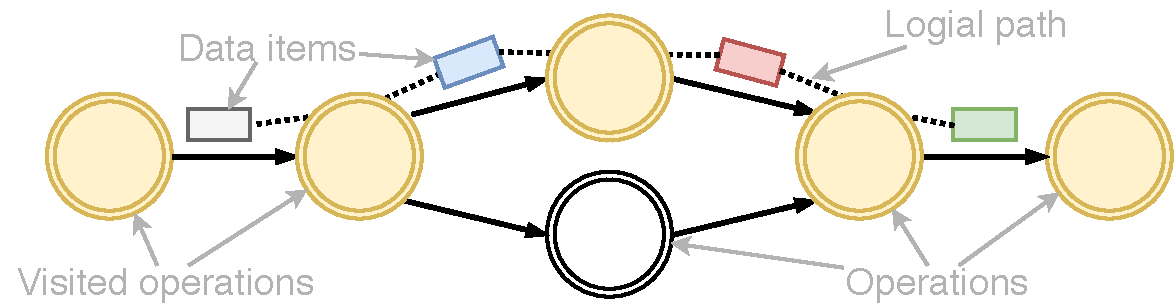
\includegraphics[width=0.9\linewidth]{Chapters/DeterministicModelRuntime/pics/logical-graph.pdf}
%     \caption{A logical execution  graph}
%     \label{logical-graph-figure}
%   \end{minipage}%
%   \begin{minipage}[b]{.5\textwidth}
%     \centering
%     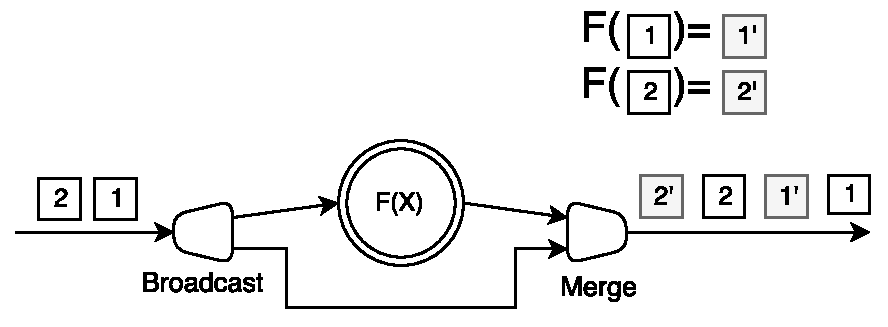
\includegraphics[width=\linewidth]{Chapters/DeterministicModelRuntime/pics/ordering}
%     \caption{The ordering model}
%     \label{ordering}
%   \end{minipage}
% \end{figure}

\begin{figure}[t]
  \centering
  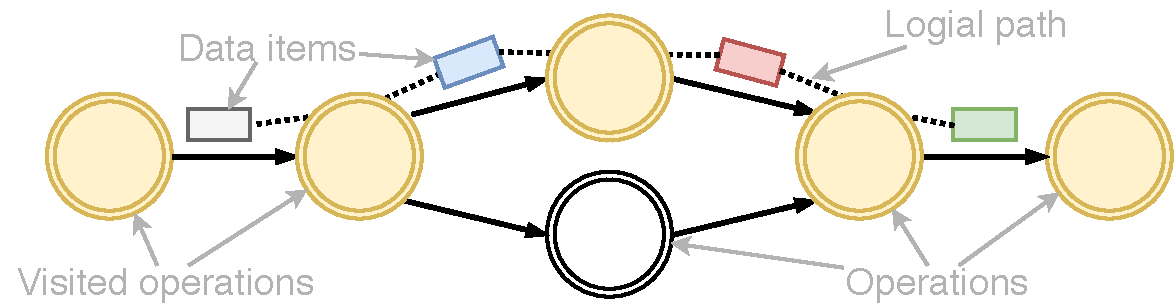
\includegraphics[width=0.8\textwidth]{Chapters/DeterministicModelRuntime/pics/logical-graph.pdf}
  \caption{A logical execution  graph}
  \label{logical-graph-figure}
\end{figure}

Data items are totally ordered according to labeles assigned to events at the entry as a part of meta-information. All operations preserve this order. Any additional items produced by an operation are placed between the item being processed and the next item. The ordering labels are dropped when items are delivered from the barrier. 

The ordering is illustrated  in Figure~\ref{ordering}. Data item with payload $1'$ is the derivative of the item with payload $1$, according to operation $F$. The same is for items with payloads $2'$ and $2$. After merge operation, the order between $1$ and $2$ is preserved. Furthermore, $1'$ follows $1$, and $2'$ follows $2$.  

\begin{figure}[t]
  \centering
  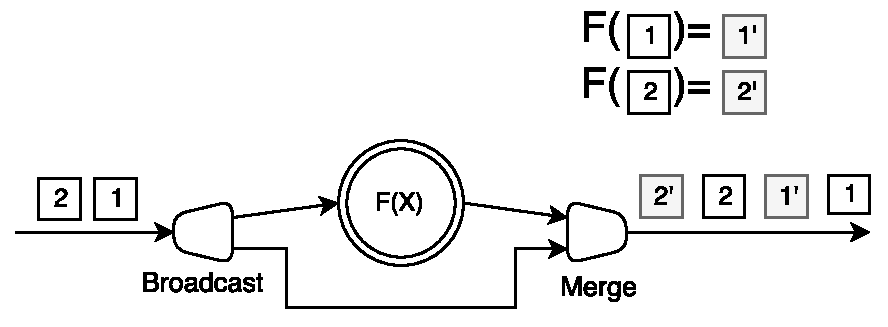
\includegraphics[width=0.7\textwidth]{Chapters/DeterministicModelRuntime/pics/ordering}
  \caption{The ordering model}
  \label{ordering}
\end{figure}

The list of available operations includes:
\begin {description}
  \item [Map] applies a user-defined function to the payload of an input item and returns a (possibly empty) sequence of data items with transformed payloads. 

  \item [Broadcast] replicates an input item to the specified number of operations.

  \item [Merge] operation is initialized with the specified number of input nodes. It sends all incoming data to the output.

  \item [Grouping] constructs a single item containing a set of consecutive items that have the same value of partition function. The maximum number of items that can be grouped is specified as a parameter  $Window Size$. 
    
  The output item of the grouping has the same ordering label as the last item in the output group. Groupings of different partitions are independent. Grouping is the only operation that has a state.
\end {description}

The following example illustrates  the grouping operation. Let the input stream be a series of integers: $ 1,2,3, \ldots$, and the  partition function returns for even numbers and 0 otherwise. If the window is set to 3, the output is 
$$(1), (2), (1|3), (2|4), (1|3|5), (2|4|6), (3|5|7), (4|6|8), \ldots$$


\subsection{State Updates}
\label{fs-drifting}

An important special case of grouping with $Window Size = 2$  provides for realization of stateful calculations with drifting state technique manifested in section~\ref{motivation-section}. Indeed, consider a map operation that follows the grouping and sends its output to the grouping input. This map operation receives a pair of its previous output considered as the state object, and new incoming item from the source stream. The map operation calculates new state object and sends it back as the grouping input. 

As an example, let us demonstrate a generic MapReduce transformation. The map stage of MapReduce can be expressed in terms of our map operation. The generic reduce stage can be presented as

\begin {tabbing}
1234\=1234\= \kill
{\bf for} $mapped \in values$ {\bf do}   \\
\>$accumulator$ := combine ($mapped$, $accumulator$); \\
{\bf end for} \\
{\bf return } $accumulator$;
\end {tabbing}

The {\it accumulator} is an explicit state that should be kept between subsequent iterations. To implement reduce stage we apply the drifting state technique and make the accumulator value a part of the stream. Figure~\ref{mapreduce-graph-figure} shows a generic graph for the MapReduce transformation. Map and reduce stages are highlighted with a dashed line. 

\begin{figure}[t]
  \centering
  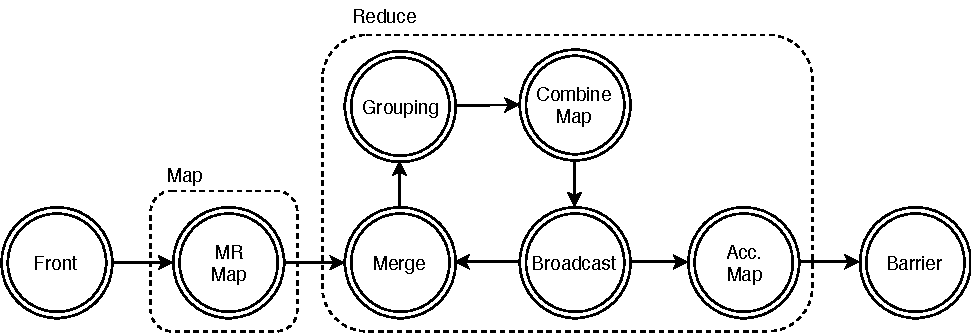
\includegraphics[width=0.8\textwidth]{Chapters/DeterministicModelRuntime/pics/mapreduce}
  \caption{Logical graph for MapReduce transformations}
  \label {mapreduce-graph-figure}
\end{figure}

There are four types of data items in this stream: {\em input}, {\em mapped}, {\em accumulator}, and {\em reduced}. The operations of the stream have the following purposes:

\begin{itemize}
  \item The first map operation outputs mapped items according to map stage of MapReduce model.
  
  \item The grouping with $WindowSize=2$ groups the $accumulator$ with next $mapped$ item. 
  
  \item The combine map produces a new state of $accumulator$ to be sent to grouping.
  
  \item The final map converts $accumulator$ into final reduce output.
\end{itemize}

Ordering rules  guarantee that each $accumulator$  item always arrives at the grouping right before next not yet combined mapped item. The cycle gives the ability for new accumulator items to get back in the grouping operation. Thereby, the stream reacts to each input item by generating new reduced item, which contains the actual value of the reduce stage.

\subsection {Deterministic Computation}
\label {fs-collision} 

To restrict outputs to only one possible result, we impose the following  restrictions on our model: 

\begin{itemize}
  \item We require map function to be pure: return value is only determined by its input values, without observable side effects
  \item We impose a strict ordering requirement on the grouping  input
\end{itemize}

While the former can be satisfied by moderating the  business logic, the latter is foreign to the distributed systems: it is hard to ensure the right order of delivery due to asynchrony inherent for a distributed system. There are two most common methods that are used to implement order-sensitive operators: in-order processing (IOP)~\cite{Arasu:2006:CCQ:1146461.1146463, Cranor:2003:GSD:872757.872838} and out-of-order processing (OOP)~\cite{Li:2008:OPN:1453856.1453890}. According to IOP approach, each operation must enforce the total order on output elements. This method does not scale well, because it requires buffering before each, even stateless, operation within pipeline until the total order is reached~\cite{Li:2008:OPN:1453856.1453890}. OOP is an approach that does not require order maintenance if it is not needed. In the case of ordering requirements, OOP buffers input items until a special condition is satisfied. This condition is based on progress indicators such as punctuations~\cite{Tucker:2003:EPS:776752.776780}, low watermarks~\cite{Akidau:2013:MFS:2536222.2536229}, or heartbeats~\cite{Srivastava:2004:FTM:1055558.1055596}.  

Some state-of-the-art stream processing systems adopt OOP~\cite{Carbone:2017:SMA:3137765.3137777}, but they suppose that items must be buffered before each order-sensitive operation if deterministic results are required. In our system, we use an optimistic approach for handling out-of-order items, that is based on OOP, but require single buffer per computational pipeline, no matter how many stateful operations it contains.

Only the grouping operation retains a dependency on the order of incoming items. Within the  optimistic approach, we accept the fact that grouping can produce incorrect output, but we guarantee that all correct groups are eventually produced. To eventually produce all correct tuples, we use an approach called {\it repair}. If an item preceding already processed items arrives at the grouping operation, all items starting with the just arrived one are re-processed, and {\em tombstones} (invalidator) are generated for all items produced earlier for all input items processed before the new one. A tombstone for an item is the same item marked with a flag in its meta-information. Hence, it traverses over the same physical path as the invalidated item.

An example of grouping repair is shown in Figure~\ref{grouping-replaying}. The green item is out-of-order. The output consists of the new valid items  $(1, 2)$ and $(2, 3)$  and the tombstone $(1, 3)_{tomb}$ for the previously generated item.

\begin{figure}[t]
  \centering
  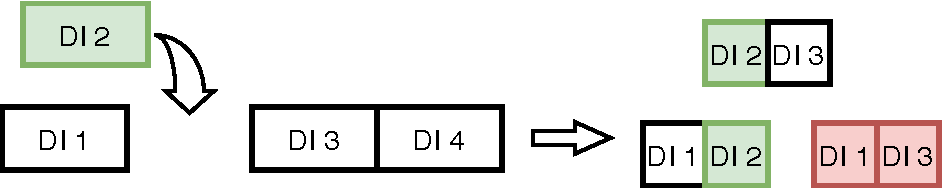
\includegraphics[width=0.6\textwidth]{Chapters/DeterministicModelRuntime/pics/grouping-replaying}
  \caption{The repair in grouping with $WindowSize = 2$.}
  \label {grouping-replaying}
\end{figure}

The barrier  keeps outgoing items on hold and filters out invalid elements, when corresponding tombstones arrive. As soon as no tombstones preceding certain point cannot arrive anymore, items are delivered  up to this point. More details can be found  in section~\ref{fs-impl}.



\section{Drifting State Implementation}
\label{fs-impl}
%%% fs-run-time-impl Implementation

We implemented the drifting state model within \FlameStream\ stream processing system~\cite{we2018beyondmr}. \FlameStream\ is implemented in Java, using Akka framework for messaging. There are several main components within the implementation:
\begin{description}
  \item[Data producers and data consumers] are deployed separately and play the role of data source and data sink correspondingly.

  \item[Graph] is a component that is deployed on each node and executes a computational pipeline defined by a logical graph. Operations within the same node communicate with each other via direct function calls for performance optimization.

  \item[Barrier] filters out invalid data items. Besides, it delivers output items to data consumers.

  \item[Acker] tracks data items within the stream. Its functionality is detailed further.

  \item[Apache ZooKeeper] is used for cluster management. The usage of ZooKeeper mitigates the need for the dedicated master node.

  \item[Persistent storage] is needed for recovery in case of failures
\end{description}

The overall scheme of the system components is shown in Figure~\ref{system-architecture}.

\begin{figure}[t]
  \centering
  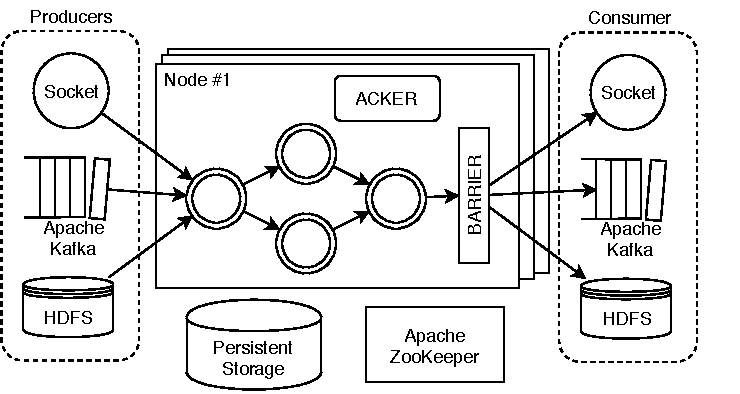
\includegraphics[width=0.9\textwidth]{Chapters/DeterministicModelRuntime/pics/arch.pdf}
  \caption{The overall scheme of the system components}
  \label {system-architecture}
\end{figure}

\subsection{Ordering model}
The meta-information of data item is implemented as a tuple of a {\it global time}, a {\it trace}, {\it child ids} and a {\it tombstone flag}.

\[Meta := (GlobalTime, ChildIds[\:], Trace, IsTombstone)\]

Global time is assigned to data item once the item enters the system. It is a pair of logical time and the identifier of the front. The identifier is used to resolve time collisions within different fronts. It is important to notice that we do not rely on any clock synchronization between nodes. The only implication of the clock skew is the system degradation regarding latency: 1 ms of the fronts clock difference appends 1 ms to minimal latency.

Each map operation can produce multiple items from one.  An ordinal number, child id, is stored in the meta information to differentiate them. {\it ChildIds} is an array of child ids, that corresponds to all visited map operations.

The global time and child ids are enough to identify data item within a stream if all processing is done in-order. In this case, if we compare global time and child ids lexicographically the meta has the desired properties that were defined in section~\ref{model-section}. 

In order to filter out all invalid data at the barrier, there is a need to match tombstones with corresponding invalid items. However, if any grouping repairs happened during processing, multiple items with the same global time and child ids exist in the stream. To differentiate them without direct payload comparison, there is a {\it Trace} value stored in the meta-information. The trace is a xor of all physical operations' ids (random 64-bit identifier) visited by item so far. Invalid item and the corresponding tombstone go along the same path because they have the same payload and the balancing functions are deterministic. Therefore, item and the corresponding tombstone can be revealed via trace matching. 

\label{mininal-time}

\subsection{Minimal time within stream}

To release an item from the barrier we need to ensure that there are no in-flight tombstones for that item, i.e., tombstones which have been already generated but have not arrived at the barrier yet.

% \newtheorem{minimal-time-claim}{Lemma}

\begin{theorem}
  For any data item $x$ let $t(x)$ be its global time. If data item $x$ has global time $t(x) < t(f)$ for each in-flight element $f$, then all tombstones for that item had already arrived at the barrier.
\end{theorem}

\begin{sketch}
  Let $x_{tomb}$ be a tombstone for {\it x}. According to the definition of the tombstone item, $t(x_{tomb}) = t(x)$, hence $x_{tomb}$ is not in-flight.
  
  New tombstones for $x$ cannot be generated because items with global time greater than $t(x)$ cannot trigger repair that affects $x$. This implies that if the stream does not contain items $x\prime$ such that $t(x\prime) \le t(x)$, then all tombstones for $x$ had already arrived at the barrier.
\end{sketch}

Therefore, to output an item from the barrier, we should ensure that there are no items in the stream with the global time less than or equal to the global time of this item.

To track the global time of in-flight items we adopt an idea of {\it acker task} inspired by Apache Storm~\cite{apache:storm}. Acker tracks data items using a checksum hash, called {\it XOR}. When the item is sent or received by an operation, its global time and checksum are sent to the acker. This message is called {\it ack}. Acker groups acks by a global time and xors received checksum hashes. When an item is sent and later received by the next operation, xoring corresponding {\it XOR}s would yield 0.

Acks are overlapped to nullify {\it XOR} only when an item arrives at the barrier. That is, ack for receive is sent only after both processing and the ack sending for the transformed item are done, as illustrated in Figure~\ref{acker}. This technique guarantees that the {\it XOR} for some global time is equal to zero only if there are no in-flight elements with such global time.

\begin{figure}[t]
  \centering
  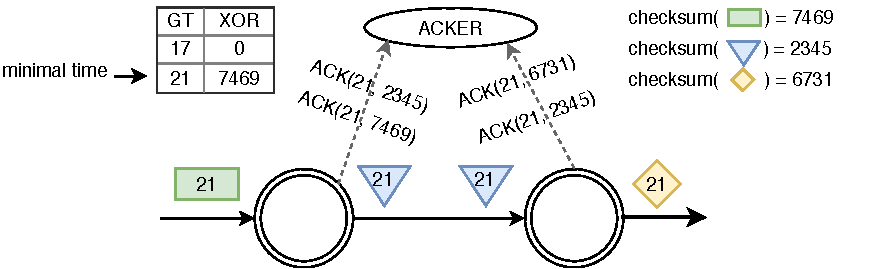
\includegraphics[width=0.8\textwidth]{Chapters/DeterministicModelRuntime/pics/acker.pdf}
  \caption{The example of tracking minimal time using acker}
  \label {acker}
\end{figure}

The minimal time within a stream is the minimal global time with non-zero {\it XOR}. On minimal time changes, acker broadcasts the {\it new minimal time notification}. Therefore, the barrier can release elements with global time $t(x)$ once it received a notification with time greater than $t(x)$.

To ensure that no fronts can generate item with the specific timestamp, each front periodically sends to acker a special message called {\it heartbeat} indicating that front will not issue items with a timestamp lower than the reported. The value in the ack table can become zero only after the corresponding heartbeat arrives.

In Chapters~\ref{thesis-chapter-substreams-consistency} and~\ref{thesis-chapter-tracker}, we generalize the concept of acker to address the substream management problem. We demonstrate that an architecture featuring a dedicated agent for progress tracking can be more efficient than the current state-of-the-art alternatives.

\section{Exactly-once Based on the Drifting State}

\section{Experimental Study}

\section{Summary}

\chapter{Substream Management}
\label{thesis-chapter-substreams-consistency}
\lhead{\emph{Substream Management}}
% Distributed stream processing engines (SPEs), such as Flink~\cite{carbone2015apache}, Heron~\cite{Kulkarni:2015:THS:2723372.2742788}, or MillWheel~\cite{Akidau:2013:MFS:2536222.2536229} aim to process intensive data streams at scale. They are deployed on clusters consisting of tens or even hundreds of nodes that receive input data elements one by one, process them, and update the internal state. These systems distribute data elements among all computational nodes in a cluster. Therefore, it is a challenging task to detect that a substream terminates system-wide. 

In Chapter~\ref{thesis-chapter-literature-review}, we introduced the notion of a substream and demonstrated that detecting substream termination is crucial for ensuring the completeness of results. This, in turn, is an important part of result consistency. The following scenarios illustrate the practical importance of this problem.

\noindent {\bf Windowed aggregations}. One way to adapt a relational query to a streaming environment is to run it on a window of data elements. This way, an initial stream will be converted into a stream of query results for each window instance. This method is widely applied in online analytics~\cite{traub2018scotty} and is used for streaming SQL implementation~\cite{Begoli:2019:OSR:3299869.3314040}. The window definition, in this case, forms a substream. For example, a sliding window will define a substream for each message in the initial stream.

\noindent {\bf State pruning}. Most SPEs group a state by keys. SPEs use them for data partitioning. For example, the task is to aggregate news into stories assigning every news item a story tag. In this case, a story tag will be the key; the properties of the story that are needed for the tagging procedure will be the state. The number of stories is not limited, and to prevent overflow~\cite{Tucker:2003:EPS:776752.776780}, SPE can remove state for outdated keys, e.g., for completed stories. In this case, the stream is a mixture of substreams: one per story.  

\noindent {\bf State snapshotting}. Epoch-based state snapshotting is a popular recovery technique applied in Flink~\cite{Carbone:2017:SMA:3137765.3137777}, Storm~\cite{Toshniwal:2014:STO:2588555.2595641}, Samza~\cite{Noghabi:2017:SSS:3137765.3137770}, IBM Streams~\cite{jacques2016consistent}. This method divides a stream into a sequence of data element chunks called ({\em epochs}). When a regular epoch is {\em atomically} processed, an SPE takes a state snapshot. In case of failures, SPE can consistently recover the state from the snapshot~\cite{2015arXiv150608603C}. 

Each of these scenarios is a particular case of a problem of monitoring substreams emergence and termination that we call a {\em substream management problem}. A substream is a part of the stream such that all its elements satisfy some predicate. 
For example, in the case of state pruning, the predicate is {\em [a data element key equals to $K$]}, for time window aggregations, the predicate is {\em [a data element has a timestamp less than $T$]}, and for state snapshotting it is {\em [a data element belongs to the epoch $E$]}.

We focus only on two signals: substream start and its termination. Tracking a start of a substream is a straightforward task: the first event of a substream will naturally trigger its start. On the contrary, generating a substream termination event is a challenging task, and practical problems may require various properties:
\begin{itemize}
    \item Deterministic windowed join\footnote{given the identical sequences of input tuples, the identical output tuples will be produced} requires an order of termination signals to respect the order of input elements (termination events from data producers)~\cite{najdataei2019stretch, gulisano2016scalejoin}.
    \item An epoch is a substream that an SPE should process atomically. A termination event for an epoch should arrive before any elements of the next epoch~\cite{2015arXiv150608603C}.
    \item State pruning problem does not require any specific properties from termination events. However, late termination event receiving may cause sub-optimal memory utilization.
\end{itemize}

In this chapter, we design a formal model for the substream management problem, estimate the network traffic overhead for state-of-the-art substream management framework, and show the theoretical lower for the traffic overhead in this task. We also formally define properties of a substream management technique required by various problems, such as state snapshotting, to ensure that a newly proposed method satisfies them. 

We organize the rest of the chapter as follows: 
Section~\ref{fs-acker-preliminaries} formalizes the substream management problem and indicates its main properties. We reveal the optimal traffic overhead for the problem in Section~\ref{fs-acker-optimal}. In Section~\ref{fs-acker-punctuations}, we discuss state-of-the-art punctuation framework and demonstrate the properties of this substream management solution in terms of our formal model. We summarize the chapter in Section~\ref{fs-acker-summary}.

\section{Formal Model of Substream Management}
\label{fs-acker-preliminaries}
First, in this section, we formalize a stream processing engine based on Chandy-Lamport distributed system definition. This model is more low-level than the model introduced in~\ref{fs-formalism} since it covers messaging between processes. Finally, we define the substream management problem based on the notions from the proposed model.

\begin{table}[!b]
\begin {center}
    \caption{Notations used throughout the chapter}
    \footnotesize
    \begin{tabular}{l|p{8.5cm}}
        \hline
        $p$ & Process (node in a physical execution graph) \\ 
        \hline
        $I_p$, $O_p$ & input and output channels of a process $p$ \\ 
        \hline
        $func_p(U, M)$ & User-defined operator run by process $p$. It receives current operator state $U$ and an incoming message $M$ \\ 
        \hline
        $\Pi$ & The set of all processes  \\
        \hline
        $K$ & Number of substreams (can be unlimited if substreams are regularly created) \\
        \hline
        $c$ & A network channel between processes  \\
        \hline
        $\mathcal{E}$ & The set of all network channels  \\
        \hline
        $s_p = U_p \cup B_p$ & State of the process $p$ consists of a mailbox $B_p$ and a state $U_p$ of $func_p$ \\
        \hline
        $mbc_{p}$ & Mailbox controller of a process $p$ \\
        \hline
        $e_{p}$ & Event of a process $p$ \\
        \hline
        $Pred(e)$ & Propositional formula defined on events \\
        \hline
        $pred(M)$ & Propositional formula defined on messages\\
        \hline
        $t(M)$ & Coarse time label \\
    \end{tabular}
    \label{notations-substreams}
\end {center}
\end{table}

\subsection{Distributed Streaming Model}
\label{fs-acker-spe-model}

Typically, distributed stream processing engines are shared-nothing runtimes that continuously ingest input elements, transform them according to a logical dataflow graph, and deliver output elements. The logical dataflow graph consists of user-defined operators. Operators are functions of a single input data element that produce output data elements. Operators can be stateless or stateful: output elements may depend on the current state. An SPE maps a logical graph to a physical (distributed) graph on deployment. Commonly, a single logical operator can be deployed on multiple computational nodes. Further, we denote physical instances of logical operators as {\em processes}.

We can describe a deployed physical graph as a distributed system in Chandy-Lamport model~\cite{Chandy:1985:DSD:214451.214456, carbone2018scalable}. In this model, the authors introduce \textit{events} that allow observing the entire system's state. This approach allows defining system-wide guarantees: in the original paper, authors used it to introduce the notion of {\em consistent state}. We use this approach for the definition of a substream management problem.

Following the notation from~\cite{Chandy:1985:DSD:214451.214456, carbone2018scalable}, one can observe a distributed system with events. 

\begin{definition}[Event]
An event is a tuple of 5 elements $e = (p, s, s', c, M)$, where $p$ is one of the deployed processes, $s$ and $s'$ are the state of the process before and after processing, $c$ is one of network FIFO channels that connect processes, and $M$ is a message generated during processing.
\end{definition}

The generated event $M$ comes to a channel state $C$ until the destination process receives it. Processes and channels form a physical graph of the system $G=\{\Pi,\mathcal{E}\}$. We denote all input channels as $I_p$ and output channels as $O_p$.

In a stream processing engine, we need to specify a process $p$ to reflect the nature of SPE. 

\begin{definition}[Process]
A process in an SPE is an actor consisting of {\em business logic handler} (BLH) and {\em mailbox controller} (MBC). The first block encapsulates a user-defined operator. The user-defined operator does not directly communicate with other processes in the system. Instead, it receives and generates {\em messages} -- data elements tagged by their source and destination. The mailbox controller handles further delivery of these messages along the communication channels and preserves the order of message generation.
\end{definition}

Figure~\ref{fig:spe_process} illustrates the scheme of a process. This system layout is not new and is widely used in practice (Akka, YDB, Millwheel, etc.).

\begin{figure}[t]
  \centering
  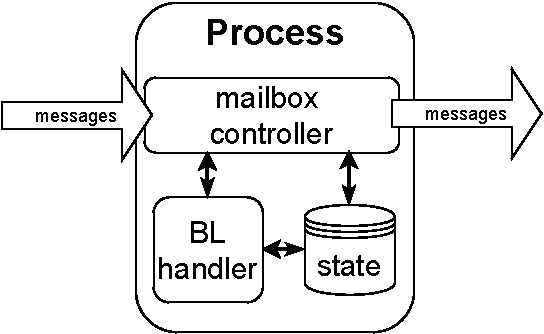
\includegraphics[width=0.6\textwidth]{Chapters/SubstreamConsistency/pics/process-scheme.pdf}
  \caption{Structure of the SPE process}
  \label{fig:spe_process}
\end{figure}

\subsection{Stream Processing Events}

When a process receives a message, the mailbox controller puts it into a particular segment of the process state ({\em mailbox} $B_p$). The business logic handler gets a message provided by MBC and triggers a user-defined operator. The user-defined operator processes the data element that the message contains and generates an arbitrary number of outgoing messages. BLH puts generated messages back in a mailbox. MBC sends outgoing messages along communication channels to destination processes. All mailbox controller operations respect the order of messages in the mailbox. If a user-defined operator has a state $U_p$, the joined process state will consist of the mailbox and this state $s=U_p \cup B_p$. In the Chandy-Lamport paradigm, this algorithm produces the following events within a process:
\begin{itemize}
    \item Communication events: $\langle recv, p, M\rangle$, $\langle send, p, M \rangle$ -- these events are handled by mailbox controller
    \item Processing of an incoming message $\langle proc, p, M, M' \rangle$
\end{itemize}

Let us translate these events into 5-tuple language. Communication events move a message between the communication channel and the mailbox section of the state:

\begin{equation}
\langle recv, p, M\rangle = (p, s_p, s'_p = U_p \cup \left(B_p \cup \{M\}\right), c_{qp}, M)
\end{equation}

\begin{equation}
\langle send, p, M \rangle = (p, s_p, s'_p = U_p \cup \left(B_p\setminus\{M\}\right), c_{p, dst(M)}, M)
\end{equation}

This function translates a destination of an element from logical dataflow graph nodes to physical communication channels between processes. Note that we need to be able to get a destination process directly from the message $dst(M)$. A practical case of this abstraction is a sharding scheme for some key: a user-defined procedure emits an event for some key, and a system is responsible for finding a proper physical channel to deliver this message.

Incoming message processing does not influence the communication channels and only ingest results of a message processing $(U', M') = func_p(U, M)$:
\begin{equation}
    \langle proc, p, M, M' \rangle = (p, s_p, s'_p = U'_p \cup \left(B_p \setminus \{M\} \cup M' \right) , \emptyset, \emptyset)
\end{equation}

Note that in this case, $M'$ may contain multiple messages. Following the Chandy-Lamport model, we assume processes are single-threaded, so within the specific process $p$, all events are ordered by a local causal order relation $<_p$: $e^{0}_p,e^{1}_p,\ldots,e^{i}_p,\ldots$. Please note that each process has its own local causal order relation, so we do not assume any total order among events from different processes. This model is indeed practical, e.g., implemented in actor-based systems.

\subsection{Substream Lifespan}

We want to get a substream's first and last element for each process. One can easily find the first one when it emerges, but verification that there will be no more events of a substream could be problematic. The strict substream termination guarantee consists of two parts: the source must promise that no more messages from the substream may emerge, and the system must ensure it contains no substream messages. The first task requires a contract with a particular data source and is thus out of scope for this chapter, though it is discussed in relevant literature~\cite{awad2019adaptive}. Instead, we focus on the second task; this is challenging due to distributed nature of the system and the absence of a standard message lifetime limit. This difficulty increases with the introduction of cycles into dataflow. Crucially, processes are not isolated, and substream messages can move from one process to another. That is why we need to observe all in-flight messages in the system.

\begin{definition}[Substream]
All events in a system satisfying a propositional formula $Pred(e)$ form a substream.
\end{definition}

We have to use system events as they are ordered inside each process and can define a border of a substream. Sometimes it is more practical to induce this predicate to messages ($pred(M)$) involved in processing: $Pred(e) = (e = \langle proc, p, M, M'\rangle) \wedge pred(M)$.

We consider substreams with a limited lifespan within a process. We want to know when a substream starts and terminates: 

\begin{equation}
\forall p, \exists t_0^p, t_1^p: \exists e: e_{t_0^p} <_p e <_p e_{t_1^p}, Pred(e) \And \forall e': e_{t_1^p} <_p e', \neg Pred(e') 
\end{equation}

We can boil this formula down: for each process $p$ in the system, there must be two event indices $t_0^p$ for substream start and $t_1^p$ for its termination, such that events satisfying $Pred$ must be between them. 

\begin{definition}[Substream Management Problem]
A substream management problem is to estimate a substream bound for each process. To indicate the bound of a substream for a process, we use a termination event or end-of-substream event:
\begin{equation}
  \langle eoss, p, Pred \rangle = (p, B_p, B_p\cup eoss(Pred), \emptyset, \emptyset)  
\end{equation}
\end{definition}

Some problems require additional properties of the termination events. For example, the state pruning problem does not require any particular properties, while for the state snapshotting problem, the substream management system should detect the exact substream bound. In the following sections, we formalize these properties. 

\subsection{Soft Bound}

Many applications that apply substream management systems do not require any particular properties of termination events. In this case, we denote the guarantee provided by such events as {\em soft bound} because termination events indicate that the substream ended some time ago.

\begin{definition}[Soft bound]
Termination event (end-of-substream) $\langle eoss_{soft}, p, Pred\rangle$ satisfies a soft bound guarantee iff:

\begin{equation}
\forall e, e >_p \langle eoss_{soft}, p, Pred\rangle \Rightarrow \neg Pred(e)
\end{equation}
\end{definition}

Figure~\ref{general_guarantees} illustrates this notion. Terms $a,b,c,d...$ denote ordered processing events of a process $p$. The substream ends after event $c$. Note that there are several other events between the end-of-substream and $c$. If $\langle eoss_{soft}, p, Pred\rangle$ occurs, all subsequent elements do not satisfy the predicate, but it is not necessarily the exact substream ``border''.

\begin{figure}[t]
  \centering
  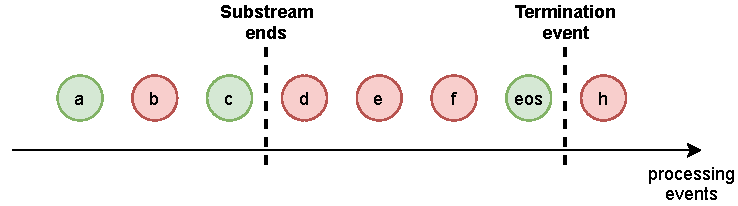
\includegraphics[width=0.75\textwidth]{Chapters/SubstreamConsistency/pics/general-guarantee.pdf}
  \caption{Substream management: soft bound}
  \label{general_guarantees}
\end{figure}

\begin{figure}[t]
  \centering
  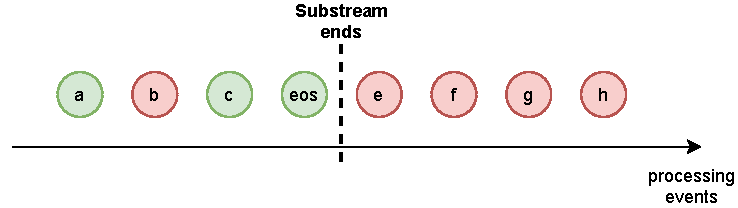
\includegraphics[width=0.75\textwidth]{Chapters/SubstreamConsistency/pics/strict-guarantee.pdf}
  \caption{Substream management: firm bound}
  \label{strict_guarantees}
\end{figure}

\subsection{Firm Bound}

The guarantee that any new event will not satisfy the predicate is sufficient for many real-life problems, e.g., SPE can initiate process state pruning on such events. However, some problems require a {\em firm bound}: guarantee that the substream ends {\em exactly} after the termination event. 

For example, a commonly used snapshotting protocol~\cite{2015arXiv150608603C, jacques2016consistent} relies on an {\em epoch}. An epoch is a special substream that must be processed atomically. Therefore, the SPE requires the termination event for a given epoch to occur immediately after the last processing event belonging to that epoch. Otherwise, the snapshot can be inconsistent, capturing elements from multiple epochs. The end-of-substream event $\langle eoss_{firm}, p, Pred\rangle$ should satisfy a {\em firm bound } guarantee to support such scenarios.

\begin{definition}[Firm bound]
Termination event (end-of-substream) $\langle eoss_{firm}, p, Pred\rangle$ satisfies a firm bound guarantee iff:

\begin{equation}
\langle eoss_{firm}, p, Pred\rangle = \inf_{<_p} \langle eoss_{soft}, p, Pred\rangle
\end{equation}
\end{definition}

Unlike the soft bound, within the firm guarantee, the first element outside the substream $Pred$ must be ordered after the firm bound event in the process $p$. This position satisfies the first possible soft bound in the events ordering. Figure~\ref{strict_guarantees} illustrates the notion of the firm bound. As in the previous example, terms $a,b,c,d...$ denote ordered processing events of a process $p$. However, in this case, event $\langle eoss_{firm}, p, Pred\rangle$ occurs right after the substream terminates.

\subsection{Consistent Termination Events Order}
Some applications require synchronization between substream termination events and substreams' last elements processing. Among these applications are epoch-based snapshotting methods and techniques for enforcing deterministic processing~\cite{we2018adbis}. For example, snapshots for consecutive epochs can be inconsistent if termination events reordering occurs. Another example is deterministic join~\cite{gulisano2016scalejoin}, which also requires the synchronized order of termination events.

Figure~\ref{notifications_reordering} illustrates termination events reordering in the case of the soft bound guarantee. Terms $a,b,c,d...$ denote ordered processing events of a process $p$. Although the substream containing events $a,b$ terminates earlier, the end-of-substream event for this substream occurs after the termination event for the substream containing events $d,e$. 

\begin{figure}[t]
  \centering
  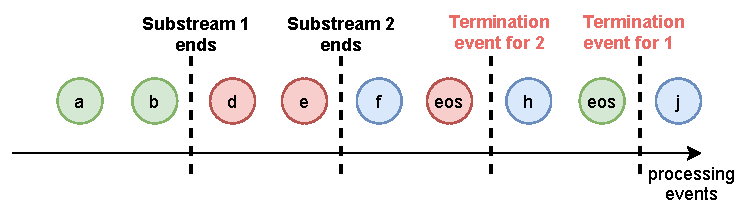
\includegraphics[width=0.75\textwidth]{Chapters/SubstreamConsistency/pics/notifications-reordering.pdf}
  \caption{An example of termination events reordering}
  \label{notifications_reordering}
\end{figure}

\begin{definition}[Consistent events order]
Let $e^{*}_1$ and $e^{*}_2$ be the last elements of substreams defined by predicates $Pred_1$ and $Pred_2$. Termination events $\langle eoss, p, Pred_1\rangle$ and $\langle eoss, p, Pred_2\rangle$ are {\em consistently ordered} iff:

\begin{equation}
e^{*}_1 >_p e^{*}_2 \Leftrightarrow \langle eoss, p, Pred_1\rangle >_p \langle eoss, p, Pred_2\rangle
\end{equation}
\end{definition}


\section{Optimal Traffic Overhead}
\label{fs-acker-optimal}
A vital performance property of a substream management system is the amount of extra network traffic. Let $|\Pi|$ be the number of processes, and $K$ be the number of substreams~\footnote{number of all created substreams, no matter if they exist concurrently or not}. 

\begin{lemma}
The network overhead induced by a substream management system cannot be lower than $O(K|\Pi|)$. 
\end{lemma}
\begin{proof}
Assume one-by-one substreams processing (e.g., epochs). When a substream management system detects the termination of a substream, each stateful process should be informed about this. Hence, each process must receive at least one network message (termination notification) for each substream.
\end{proof}

In this proof, we assume that each process should be informed about substream termination, while some processes may not require such notifications, for example, if they are stateless. This assumption is realistic because, as we mentioned in Section~\ref{fs-acker-spe-model}, logical operators are commonly deployed on each computational node, e.g., in state-of-the-art SPEs such as Flink~\cite{Carbone:2017:SMA:3137765.3137777}, Storm~\cite{apache:storm}, Samza~\cite{Noghabi:2017:SSS:3137765.3137770}. In this model, each process must receive the substream termination event because each process handles all logical operators.

\section{Punctuation Framework}
\label{fs-acker-punctuations}
In this section, we show how our model can describe the most widely used substream management framework called {\em pucntuations}. We also prove specific properties that are inherent to any implementation of the punctuation framework. 

\subsection{Framework Overview}

The main idea behind the punctuation framework is to inject special data elements $\mathcal{P}^{pred}$ into the data stream one per substream. These elements, called punctuations, flow down the workflow as ordinary data elements. The injector promises that all elements after punctuations will not satisfy the predicate. Hence, the punctuation itself defines the ``border'' of a substream.

Figure~\ref{punctuations_scheme} illustrates the punctuation framework. Punctuations are delimiters between the substream elements and all other items. Green elements indicate elements that belong to some substream, while red elements do not.

\begin{figure}[t]
  \centering
  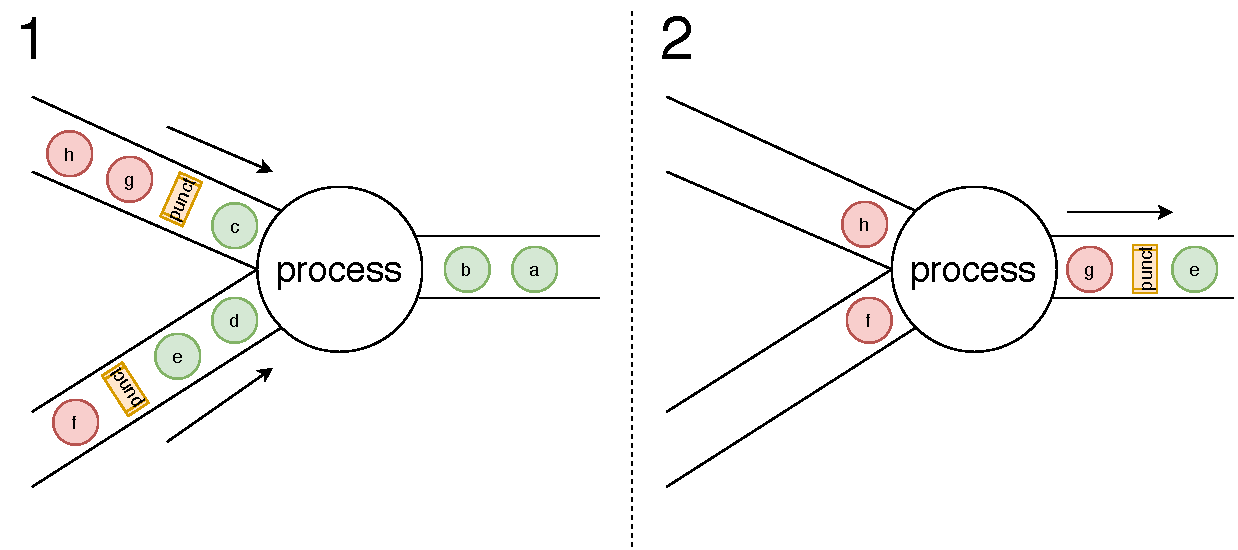
\includegraphics[width=0.80\textwidth]{Chapters/SubstreamConsistency/pics/punctuations-scheme.pdf}
  \caption{Punctuations handling by a single process}
  \label{punctuations_scheme}
\end{figure}

Processes within SPE do not apply user-defined operators to punctuations. Instead, each process $p$ propagates punctuation messages $\mathcal{P}_{pq}^{pred}$ to all outgoing channels $c_{pq} \in O_p$  when it receives corresponding punctuations from all input channels $I_p$.

\subsection{Substream Termination Events}

\begin{lemma}
Generating an event by the following rule ensures the soft bound of a substream $pred$:
\begin{equation}
\forall q \in I_p, \exists \mathcal{P}^{pred}_{qp} \in B_p, \forall M\in B_p : \neg pred(M) \vee dst(M) \ne p
\end{equation}
\end{lemma}

\begin{proof}
We can use indirect proof. Let $\langle proc, p, M^*, M' \rangle$ be a processing event that happens after the soft bound termination event but $pred(M^*)$. In other words, a message $M^*, pred(M^*)$ arrived after all punctuations for the predicate $pred$ had arrived. According to the definition of a distributed system from Section~\ref{fs-acker-spe-model}, message $M^*$ could emerge either from the mailbox of a process or incoming channels. The emergence from the mailbox contradicts the condition of the termination event generation rule $\forall M\in B : \neg pred(M) \vee dst(M) \ne p$.
Conversely, if an element comes from an incoming channel, we can track its path through the system from a data source to the channel (processing path). Because of broadcasts on each step, punctuations travel all possible paths in the system, including the path that traveled the element. Along this path, they were reordered. It could happen either during transmission or during processing. The first hypothesis contradicts the FIFO nature of communication channels. The second one is impossible due to the definition of the processing model that protects a processing order. We have excluded all possible ways of getting event $M^*$ and must reject the initial hypothesis.
\end{proof}

To satisfy the firm bound guarantee, the mailbox controller should block the processing of all incoming messages from a channel as soon as it receives punctuation from this channel. In~\cite{Carbone:2017:SMA:3137765.3137777}, such behavior is called {\em watermark (punctuation) alignment}. Formally we can rewrite this requirement in terms of event ordering:

\begin{lemma}
A soft bound becomes firm if a process event order satisfies the following conditions:
\begin{equation}
\label{eq:firm_condition}
\forall e_1, e_2 = \langle recv, p, \mathcal{P}^{pred}_{q_{1,2}p} \rangle, \nexists e' = \langle proc, p, M_{q_1p}, M' \rangle, e_1 <_p e' <_p e_2
\end{equation}
\end{lemma}
\begin{proof}
Suppose a message $M_{qp}$ of the next substream was processed after the last element of the current substream but before the generation of a bound event. This message either came from the channel $q$ before the punctuation from that channel or was processed before all channels delivered their punctuations. The first case could happen if $M_{qp}$ was reordered with the punctuation along the processing path and contradicts FIFO processing logic (see previous proof for details). The second case is impossible because of processing limitations introduced by~\ref{eq:firm_condition}.
\end{proof}

\subsection{Properties of the Punctuation Framework}

The design of the punctuation framework implies two important properties:

\begin{enumerate}
    \item {\bf Lack of cyclic dataflows support.} Although there are techniques that extend punctuations for state snapshotting of iterative processing~\cite{Carbone:2017:SMA:3137765.3137777}, the termination of a general substream cannot be determined using the punctuation framework if an execution graph contains cycles.
    \item {\bf Network traffic complexity quadratically depends on the number of processes.} As we demonstrated above, each process waits for punctuations from all incoming network channels delivers. It leads to high network traffic overhead if all processes are interconnected.
\end{enumerate}

\begin{lemma}
The punctuation framework cannot determine a substream termination of an execution graph if the graph contains a cycle.
\end{lemma}
\begin{proof}
If we have a cycle in the processing graph, we can find a process that receives input from the latter steps of the cycle (back-link). This process will propagate a punctuation element when all incoming channels have received their punctuation elements. Due to the cycle, this punctuation element processing path contains the process itself (as a starting element of the cycle). It means that we need the punctuation to be already generated to generate it. We obtained a contradiction.
\end{proof}

Despite the previous Lemma, some punctuation-based systems report support of cyclic workflows. One can practically achieve it by limiting the number of possible entrances into the cycle by some $m$. With this limitation, we can roll out the cycle with repeating fragments of the cycle $m$ times. The first block is then connected to the input of the cycle, and the last element of the cycle to two elements: repetition entrance and the output of the cycle. Repetitions are organized the same way. Theoretically, this cycle representation is a DAG so that the punctuation mechanism can serve it.

For example, the technique proposed in~\cite{Carbone:2017:SMA:3137765.3137777} allows SPEs to use punctuations for the state snapshotting problem. The main idea of this technique is to include in a snapshot all in-transit elements (possibly from previous epochs) within a cycle and then resend them on rollback. It is the specific form of the limitation on the number of possible entrances with $m=1$.

\begin{lemma}
Network traffic complexity for this method is $O(K|\Pi|^2)$, where $|\Pi|$ is the number of processes and $K$ is the number of substreams if an SPE distributes the work among processes evenly.
\end{lemma}
\begin{proof}

Even the soft bound event requires receiving punctuations from all incoming network channels. If a distributed stream processing engine balances the work evenly among the processes, all processes are interconnected. Therefore, each active process should broadcast punctuations to all other processes. Assuming that all processes handle the elements belonging to the predicate, the transmission complexity of punctuation elements is $O(K|\Pi|^2)$. Therefore, if the number of existing substreams is $K$, then the network traffic complexity for the punctuation framework is $O(K|\Pi|^2)$ because each process should broadcast punctuations for each substream. 

\end{proof}

Several promising directions exist for improving the network traffic complexity for the punctuation framework. Firstly, one can batch punctuations for several substreams if they do not require independent termination events. It can reduce network complexity to $O(\frac{K}{B}|\Pi|^2)$ where B is a batching frequency. On the other hand, this approach is unsuitable for all substream types (e.g., it cannot be applied for epochs) and can increase the latency between the substream end and the termination event while keeping the quadratic dependency on the number of nodes.

Secondly, it is possible to attach punctuations to all regular input data elements. In this case, there can be no extra traffic in terms of messages at all. However, it makes the latency between the substream end and the termination event unpredictable because some network channels can rarely be used.

Both mentioned optimization ideas have significant trade-offs and require deep theoretical and experimental research. We do not elaborate on optimization ideas in this work, leaving them for future work.


\section{Summary}
\label{fs-acker-summary}
\label {fs-acker-conclusion}

In this chapter we presented a formal model for the substream management problem and established a theoretical lower bound for this overhead. We demonstrated that state-of-the-art punctuation framework is far from the theoretically optimal approach. Additionally, we showed the key properties that a substream management technique must fulfill to support tasks such as state snapshotting, ensuring that newly proposed methods adhere to these requirements.

\chapter{Tracker: Substream Management Framework}
\label{thesis-chapter-tracker}
\lhead{\emph{Tracker: Substream Management Framework}}
A popular substream management method is the punctuation framework~\cite{tucker2003exploiting} applied in many production-scale SPEs such as Flink~\cite{carbone2015apache}, Heron~\cite{Kulkarni:2015:THS:2723372.2742788}, Samza~\cite{Noghabi:2017:SSS:3137765.3137770}, IBM Streams~\cite{jacques2016consistent}, Apex~\cite{pathak2016introduction}. The main idea behind this framework is to divide the stream by injecting special elements called {\em punctuations} that define substreams ``borders''. An SPE propagates these special elements via the same network channels as data elements. While the punctuation approach is robust and easy to implement, it has several limitations. 

Punctuations are not applicable for cyclic dataflows in a general case because elements belonging to a substream can remain in transit within a cycle for an uncertain time~\cite{carbone2018scalable}. Cyclic dataflows are commonly used for the distributed implementation of iterative web-graph algorithms like PageRank or search for connected components~\cite{ewen2012spinning, murray2016incremental, mcsherry2013differential}.

The technique proposed in~\cite{Carbone:2017:SMA:3137765.3137777} mitigates this issue for the state snapshotting problem. The main idea of this technique is to include in a snapshot all in-transit elements (possibly from previous epochs) within a cycle and then resend them on rollback. However, it does not allow a system to determine a substream termination for cyclic dataflows using punctuations.

As we demonstrated in the previous chapter, the high network overhead forms another limitation. Network traffic complexity for this method is $O(K|\Pi|^2)$, where $|\Pi|$ is the number of processes and $K$ is the number of substreams because each process should propagate punctuations to all output channels. The above formula estimates the number of punctuation messages needed in the worst case of fully interconnected processes. 

We argue that the worst case can appear on any execution graph that contains a re-partitioning operator. Indeed, SPEs try to distribute workload evenly between processes~\cite{carbone2015apache, Kulkarni:2015:THS:2723372.2742788, Akidau:2013:MFS:2536222.2536229}, so elements of a substream can be evenly distributed among processes as well. When a process reaches the end of a substream, it must broadcast the punctuation because the items of the part of a sub-stream handled by this process are re-distributed evenly for subsequent processing.

Substreams can be {\em fine-grained}: for example, each user session defines a substream. If there are a lot of small substreams, an inefficient substream management system can degrade the latency~\cite{DBLP:journals/pvldb/BegoliACHKKMS21} and the throughput of an SPE~\cite{Li:2008:OPN:1453856.1453890} or affect the performance of state checkpointing~\cite{zhang2021research}.

\begin{figure}[t]
  \centering
  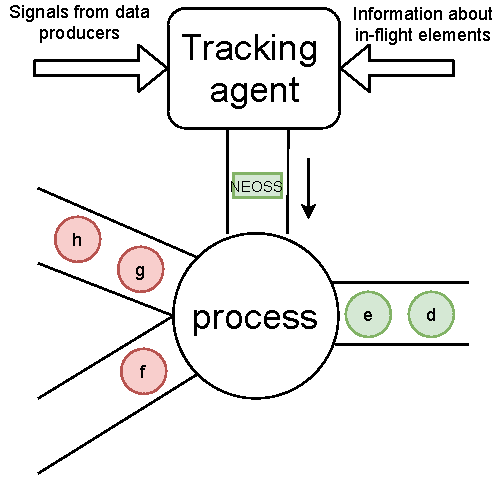
\includegraphics[width=0.60\textwidth]{Chapters/Tracker/pics/tracker-scheme.pdf}
  \caption{\tracker\ framework: tracking agent aggregates information about substreams and produces NEOSS}
  \label{tracker_scheme}
\end{figure}

In this chapter, we introduce a new substream management framework called \tracker. Figure~\ref{tracker_scheme} shows the high-level scheme of our method. 
Within this framework, we use a dedicated agent that receives information about substreams from the entire SPE and sends back {\em end-of-substream notifications} (NEOSS). 
An SPE propagates NEOSS messages through this agent without broadcasting between processes, reducing the amount of extra traffic. This propagation method is suitable for cyclic dataflows because there is no need to forward service traffic through the cycles. A distributed version of the agent allows an SPE to scale.

% In summary, our contributions are as follows:
% \begin{enumerate}
%     \item We provide a formal model of substream management. This model allows us to compare the properties of various substream management systems.
%     \item We present a novel substream management technique that achieves a lower bound of network traffic overhead.
%     \item We demonstrate \tracker\ performance compared to a state-of-the-art approach on diverse workloads.
% \end{enumerate}

% This paper is an extended version of a conference publication~\cite{10.1145/3524860.3539809}. This paper addresses a scalability problem by introducing a distributed version of the tracking agent and evaluating it on workloads with increased load. We further expand the theoretical properties of punctuation and tracker frameworks and reveal the motivation behind this work in more detail.

We organize the rest of the chapter as follows: in Section~\ref{fs-acker-tracker}, we introduce a general design of the \tracker\ framework and demonstrate the properties of this substream management solution, Section~\ref{fs-acker-impl} summarizes the implementation of \tracker\ for both centralized and distributed setups with optimizations that can reduce the amount of extra traffic, in Section~\ref{fs-experiments}, we show that the proposed technique is scalable and can outperform alternatives employed in state-of-the-art stream processing engines, Section~\ref{fs-tracker-conclusion} summarizes this chapter.

\section{Tracker Framework}
\label{fs-acker-tracker}
% This section introduces a novel substream management framework called \tracker\ that is suitable for cyclic dataflows and achieves the lower bound of network overhead. We also demonstrate that it provides all lifespan event properties defined in the previous section.

In the previous chapter we showed that the extra traffic cannot be lower than $O(K||\Pi||)$, where $|\Pi|$ is the number of computational nodes and $K$ is the number of substreams. To achieve this lower bound, one can apply an additional agent (process) that receives information about substreams from processes and sends back information about terminated substreams. 

In this case, the fact that a substream terminates is propagated through this agent without broadcasting between processes, so the amount of extra traffic can be linear by the number of processes. This propagation method is suitable for cyclic dataflows because there is no need to forward service traffic through the cycles. Therefore, we design a {\em tracking agent} that:

\begin{enumerate}
    \item Receives signals from data producers that a substream has terminated.
    \item Watches for in-flight elements and substreams.
    \item Notifies dataflow processes when the substream ends {\em for them}, i.e., when they stop receiving elements that satisfy some predicate.
\end{enumerate}

Figure~\ref{tracker_scheme} shows the general scheme of the \tracker\ mechanism. A tracking agent receives signals from data sources, fetches information about in-flight elements, and then decides where to send {\em end-of-substream notifications} (NEOSS).

In this framework, substream termination events are propagated through additional network channels physically separated from the channels used for data elements. A similar idea of using extra network channels for service messages is applied in~\cite{wang2022fries} for a runtime reconfiguration problem.

This approach can be more efficient regarding network traffic but provides new challenges. Before diving into implementation details, we should answer the following questions regarding \tracker\ framework:

{\bf Q1 How to monitor in-flight elements?} To detect that a substream ends, the tracking agent should receive the corresponding signal from data producers and ensure no substream in-flight elements. 

{\bf Q2 How to ensure bound guarantees?} While there are no longer special elements in the stream that denotes the substream end, we need to design soft and firm substream bound conditions based on NEOSS from the shared agent. 

{\bf Q3 How to provide a consistent termination events order?} Unlike punctuations, \tracker\ notifications are completely async with dataflow elements because they go through another network channel. Hence, dataflow items and notifications are not ordered, making it hard to ensure that the notifications order is consistent.

{\bf Q4 What functional and performance properties does the \tracker\ have?} \tracker\ framework is designed to eliminate the limitations of the punctuation framework. We should demonstrate that it is suitable for cyclic dataflows and can provide lower network overhead.

\subsection*{Answering Q1: How to Monitor In-Flight Elements?}
Each process sends the following report messages on each $\langle proc, p, M, M' \rangle$ event to the tracking agent:
\begin{enumerate}
    \item For all output elements $m \in M'$ for all substreams they belong to \\ $pred(m) = 1$: $SND(pred, m, p)$
    \item For the input element $M$ and all satisfying substreams \\ $pred(M) = 1$: $RCV(pred, M, p)$
\end{enumerate}
Further in this paper, we will denote them as {\em SND report} and {\em RCV report}. The order of $SND$ and $RCV$ messages is vital because each pair of these events forms a chain ring, and sending $SND$ before $RCV$ links these rings together. We can use these chains to track data element processing for a workflow graph or its part.

Chains of $SND$ and $RCV$ messages allow the \tracker\ to track the processing of a data element along with a workflow graph. This idea is based on the commutativity of XOR and used in Apache Storm Acker~\cite{apache:storm:acker}. However, despite the technical similarity of the core idea, Acker and \tracker\ play different roles in SPE. Acker ensures that the system processes an input element entirely and notifies the user when the processing runs out of time. \tracker\ tracks an entire substream and allows an SPE to detect its bounds.

\subsection*{Answering Q2: How to Ensure Bound Guarantees?}
A process must ensure that input channels will provide no more elements of this substream to detect a substream bound. In the case of the punctuation framework, the watermark messages carry this guarantee. In the case of the tracking agent, NEOSS messages play the same role. We can assume that each input channel $c$ comes from a segment of the workflow $W_c$ graph. NEOSS is sent to a process when:
\begin{itemize}
    \item for all incoming channels $c \in I_p$ corresponding segment $W_c$ contains no elements of the substream in-flight (has unpaired $SND$ report);
    \item all data providers have promised to send no more elements of the substream.
\end{itemize}
It is easy to show that we can join workflow segments for all incoming channels $W_p = \cup_{c\in I_p} W_c$ and track a single subgraph $W_p$ per process. Using the properties of NEOSS, we can define a soft bound criterion:
\begin{lemma}
The following rule generates the soft substream bound:
\begin{equation}
 \exists NEOSS \in B_p, \forall M\in B_p : \neg pred(M) \vee dst(M) \ne p
\end{equation}
\end{lemma}
\begin{proof}
If a substream data element is processed after the defined point in events order, it comes from the mailbox or one of the incoming channels $c \in I_p$. The first case contradicts $\forall m\in B_p : \neg pred(m)$. The second case could happen because a new substream element enters the system (source broke the promise) or a substream element inside the $W_p$ without the $SND$/$RCV$ chain (contradicts with $SND$/$RCV$ chains generation rule). 
\end{proof}

To satisfy the firm bound guarantee, one needs to hold elements not belonging to the substream in the mailbox until NEOSS has arrived. This technique is similar to the punctuation alignment behavior mentioned in the previous section. If this condition is satisfied, then $\langle eoss_{firm}, Pred\rangle$ = $\langle eoss_{soft}, Pred\rangle$ for the \tracker.

\subsection*{Answering Q3: How to Provide the Consistent Termination Events Order?}
\label{termination_order}
In the punctuation framework, such order is provided by design because punctuations and ordinary data items go through the same FIFO network channels. In \tracker\, this order should be enforced. Assume that SPE assigns a special totally ordered label $t(M)$ to the messages. All messages generated by single processing inherit the label from the input message. 

In this case, if the order on $t(M)$ coincides with the order of input elements, then \tracker\ can also produce the NEOSS events according to this order. In other words, \tracker\ can reorder the NEOSS events to make them consistent with the substreams order. Figure~\ref{tracker_ordering} shows an example of this concept. The substream containing element with $t=1$ ends before the substream containing element with $t=2$. As we can see, the order of NEOSS elements from \tracker\ coincides with $t(M)$.

\begin{figure}[t]
  \centering
  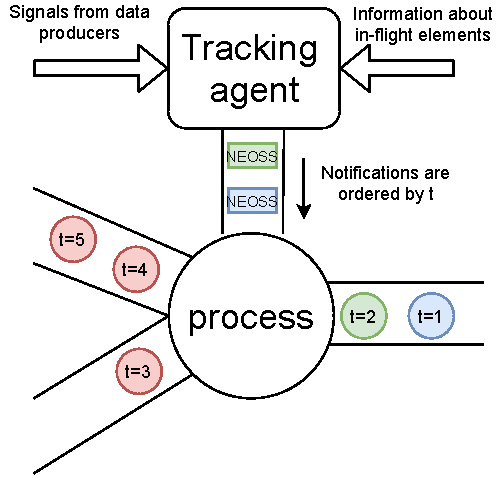
\includegraphics[width=0.60\textwidth]{Chapters/Tracker/pics/tracker-ordering.pdf}
  \caption{\tracker\ framework: tracking agent sends NEOSS elements according to the order on t(m)}
  \label{tracker_ordering}
\end{figure}

A vital question here is how to implement the assignment of ordered labels $t(m)$. One way is to use the {\em time oracle} service~\cite{10.14778/3055330.3055335}, which can provide totally ordered labels. We discuss a simple alternative in the next section. 

\subsection*{Answering Q4: What are the Functional and Performance Properties of \tracker?}
\label{tracker-properties}

\tracker\ does not require regular broadcasting of the elements to all computational nodes because all service traffic goes through a single agent. This change allows \tracker\ to have the following properties by design:

{\bf Cyclic dataflows support.} Because the tracking agent monitors the properties of in-flight elements without directly injecting service items into a dataflow, \tracker\ does not have the problem of throwing them through a cycle.

{\bf Low network overhead.} Processes can send reports once per a fixed time period, so there is a constant time of such reports per a finite substream. The reports require $O(|\Pi|)$ extra messages, while the NEOSS events $O(K|\Pi|)$. The total amount is $O(K|\Pi| + |\Pi|) = O(K|\Pi|)$, which is optimal for the substream management problem.

Both of these properties are enhancements to the punctuation framework. They lead to an important corollary: 

{\bf Low latency and impact on SPE throughput.} Punctuations can be stuck by other data elements if they are sent with some delay after the last substream element. In \tracker, service traffic goes through other network channels that can reduce latency between actual substream termination and the corresponding event. Together with the low service network traffic, this scheme does not significantly reduce the throughput of an SPE, as we show in Section~\ref{fs-experiments}.

In the next section, we theoretically prove the first two properties. We experimentally demonstrate the fairness of the corollary in Section~\ref{fs-experiments}.


\section{Tracker Implementation}
\label {fs-acker-impl}
In the previous section, we introduced a general schema of the \tracker\ framework. In this section, we deepen into its implementation details. We describe and explore the properties of the tracking agent that produces the substream termination notifications (NEOSS). After that, the technique to achieve consistent termination events order is detailed. Distributed implementation of the tracking agent concludes this part.

\subsection{Bound Guarantees}

The tracking agent splits the workflow graph into partially ordered segments and tracks them separately. For each process $p$, we can generate a list of preceding segments, including a set of incoming message generators $W_p$. As soon as all these segments contain no elements of a substream, the agent sends to a process {\em NEOSS}.

To track the message path through segments, the agent receives SND/RCV reports containing a segment identifier and a list of predicates the message satisfies. The agent aggregates this information into the table illustrated in Table~\ref{tracker-table-simple}.

\begin{table}[b]
\caption{\tracker\ table: a general example}
  \label{tracker-table-simple}
  \centering
  \footnotesize
  \begin{tabular}{|c|c|c|>{\bfseries}c|} 
    \hline
    Notified & Predicate & Segment & Substream elements  \\ \hline \hline
    \multirow{2}{*}{\checkmark} & \multirow{2}{*}{h(x)} & A & No \\ \cline{3-4}
    & & B & No \\ \hline
    \multirow{2}{*}{} & \multirow{2}{*}{q(x)} & A & No \\ \cline{3-4}
    & & B & Yes \\ \hline
    \multirow{2}{*}{\checkmark} & \multirow{2}{*}{z(x)} & A & No \\ \cline{3-4}
    & & B & No \\ \hline
  \end{tabular}
\end{table}

A graph shown in Figure~\ref{fig:tracker-acker-comparison} illustrates the notion of segments. This graph has two segments: $A$ and $B$. According to Table~\ref{tracker-table-simple}, the NEOSS for predicate $q(x)$ can be sent for a segment $A$, but not for a segment $B$. This behavior is similar to punctuations: NEOSS can be spawned earlier for the upstream processes.

\begin{figure}[t]
  \centering
  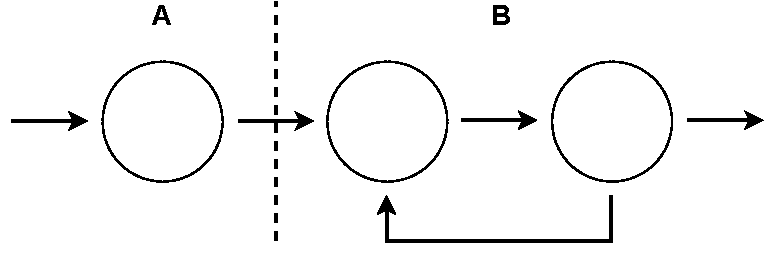
\includegraphics[width=0.6\textwidth]{Chapters/Tracker/pics/segments-example.pdf}
  \caption{Graph segmentation example}
  \label{fig:tracker-acker-comparison}
\end{figure}

Several possible methods exist to build the indicator that the segment contains elements from a substream using the reports from processes. Our implementation uses the trick applied in Apache Storm to monitor the completeness of processing~\cite{apache:storm:acker}. 

Each report is labeled by a random number $X$, the same for the send and the corresponding receive actions. This trick makes it easy to check if the segment contains a complete set of $SND$/$RCV$ pairs for a message: XOR operation for all numbers received from the chain will turn into 0. The result of the XOR operation can accidentally become zero. However, the probability of this event is controlled by the random number $X$ length so that one can neglect it in practice~\cite{apache:storm:acker}.

\begin{figure}[t]
  \centering
  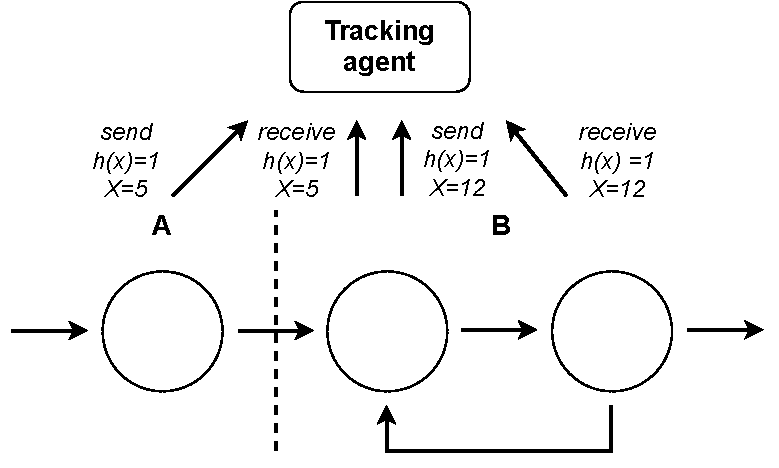
\includegraphics[width=0.6\textwidth]{Chapters/Tracker/pics/tracker-segments-example.pdf}
  \caption{Reports example}
  \label{fig:tracker-reports}
\end{figure}

Figure~\ref{fig:tracker-reports} illustrates the reports with random numbers. The elements satisfying a predicate $h(x)$ flow through a dataflow. The first process generates an output and sends the SND report with $X=5$. The corresponding RCV report by the second process also has $X=5$ because this process receives the element from the first one. The second process sends a new element that satisfies $h(x)$ to the following process and produces the new SND report with $X=12$. The third operator receives this element and produces an RCV report with $X=12$. If there are no more elements such that $h(x)=1$, then we can send NEOSS for the substream defined by $h(x)$ ends because {\em 5 XOR 5 XOR 12 XOR 12 = 0}. Table~\ref{tracker-table-xor} illustrates the actual \tracker\ table for the mentioned technique.

\begin{table}[b]
\caption{\tracker\ table: XORing technique example}
  \label{tracker-table-xor}
  \centering
  \footnotesize
  \begin{tabular}{|c|c|c|>{\bfseries}c|>{\bfseries}c|} 
    \hline
    Notified & Predicate & Segment & Segm. XOR & XOR  \\ \hline \hline
    \multirow{2}{*}{\checkmark} & \multirow{2}{*}{h(x)} & A & 000 & \multirow{2}{*}{000} \\ \cline{3-4}
    & & B & 000 & \\ \hline
    \multirow{2}{*}{} & \multirow{2}{*}{q(x)} & A & 000 & \multirow{2}{*}{110} \\ \cline{4-4}
    & & B & 110 & \\ \hline
    \multirow{2}{*}{\checkmark} & \multirow{2}{*}{z(x)} & A & 000 & \multirow{2}{*}{000} \\ \cline{3-4}
    & & B & 000 & \\ \hline
  \end{tabular}
\end{table}

\subsection{Implementation Properties}

In the \tracker\ framework, there is no need to inject service items into a dataflow. Thus, \tracker\ can handle cyclic execution graphs.

\begin{lemma}
If an execution graph is cyclic, the \tracker\ framework can determine substream termination.
\end{lemma}
\begin{proof}
Suppose an execution graph contains a cycle and no in-flight elements in the system satisfying a predicate $pred$, but \tracker\ did not provide NEOSS for the substream. It means that the corresponding XOR value is not 0. Therefore, there is a process that sends an element satisfying $pred$ (possibly through the cycle), but the following process has not received and processed it yet. We obtain a contradiction because we supposed that the execution graph does not contain an in-flight element satisfying the predicate $pred$.
\end{proof}

Another property that became reachable due to avoid of injecting service items into a dataflow is low network traffic overhead. All traffic goes between the tracking agent and processes without broadcasting service items among processes.

Due to the associativity of XOR, we can optimize tracking agent incoming traffic by aggregating reports locally within the processes. For each process, we introduce a {\em local tracking agent} component. It serves as a mediator between the process and the global agent, buffering the outgoing reports and flushing them periodically. 

\begin{lemma}
Network traffic complexity for the \tracker\ framework is $O(K|\Pi|)$, where $|\Pi|$ is the number of processes and $K$ is the number of substreams.
\end{lemma}
\begin{proof}
Substreams last a finite time period by definition so that each process sends aggregated reports a constant number of times that does not depend on the number of substreams and processes. Therefore, the amount of extra network traffic for the reports is $O(|\Pi|)$, so the total estimation with the overhead on the notifications is $O(K|\Pi|)$ because \tracker\ must inform all processes about substream termination (send NEOSS).
\end{proof}

The flushing window is the parameter that allows us to balance the service traffic and latency between the actual substream termination (the event from the data producer) and the termination event. Although this optimization does not reduce the theoretical estimation of network traffic complexity, it can significantly reduce substream termination latency, as demonstrated in Section~\ref{fs-experiments}.

\subsection{Consistent Termination Events Order}
\label{termination_order_impl}

If the order of NEOSS is consistent, the order of termination events will also be consistent. To achieve consistent order of NEOSS, we need to define $t(M)$ such that the order on $t(M)$ respects the order of input elements. All reports that processes send to the tracking agent should be labeled with $t(M)$. The tracking agent sends the NEOSS elements according to the order on $t(<)$.

Table~\ref{tracker-table-oder} illustrates the \tracker\ table in case of consistent NEOSS order. Column {\em min t(x)} indicates the minimal $t(x)$ among the elements that satisfy the corresponding predicate. The tracking agent sends notifications for the substream if the $XOR$ value is 0 and all substreams that contain elements with less {\em min t(x)} have finished (notifications have been produced). Therefore, NEOSS for the substream defined by the predicate $h(x)$ is not sent until the NEOSS for the predicate $q(x)$ is generated. 

\begin{table}[b]
\caption{\tracker\ table: consistent NEOSS order example}
  \label{tracker-table-oder}
  \centering
  \footnotesize
  \begin{tabular}{|c|c|>{\bfseries}c|c|} 
    \hline
    Notified & Predicate & min t(x) &  XOR  \\ \hline \hline
    \multirow{2}{*}{waits for q(x) finish} & \multirow{2}{*}{h(x)} & \multirow{2}{*}{5} & \multirow{2}{*}{000} \\
    & & & \\ \hline
    \multirow{2}{*}{} & \multirow{2}{*}{q(x)} & \multirow{2}{*}{4} & \multirow{2}{*}{110} \\
    & & & \\ \hline
    \multirow{2}{*}{\checkmark} & \multirow{2}{*}{z(x)} & \multirow{2}{*}{1} & \multirow{2}{*}{000} \\
    & & & \\ \hline
  \end{tabular}
\end{table}

If input elements arrive through a single node, $t(x)$ can denote the monotonic system time of the element $x$ arrival. If there are multiple source processes, one can use time oracle agent~\cite{10.14778/3055330.3055335} as a service for the generation of a monotonic sequence of unique timestamps. However, in this case, there is a need to manage one more subsystem.

A simple technique to build $t(x)$ without extra agents is based on systematic synchronization of the system clocks. We call this method and associated labels {\em coarse time}. Assume that clock differences are no more than some fixed $\delta$, which we reference as synchronization slack. Let $\tau(x)$ be a precise physical time of input data item $x$ arrival, and $s(x)$ be the local system time of the source node where $x$ arrived. The valid order of events $\tau(d_1) > \tau(d_2)$ coming from different sources can sometimes be restored by their system timestamps $s(d_1)$ and $s(d_2)$. If these timestamps differ more than time synchronization slack, then the order is clear: $s(d_1) > s(d_2) + \delta \Rightarrow \tau(d_1) > \tau(d_2)$.

This fact allows us to define $t(x)$ such that $t(x) = [s(x) / \delta]$. This way, we make $t(x)$ less precise, but this trick allows us to compare global time assigned by different source nodes. If $t(x_1)$ is greater than the $(t(x_2) + 1)$, then their order is defined even if they arrived from different source nodes:  $t(x_1) > t(x_2) + 1 \Rightarrow \tau(x_1) > \tau(x_2)$. Therefore, the order on $t(x)$ coincides with the order of input elements, so it is suitable for the defined problem. Here is a summary of the mechanism that ensures consistent termination events order:
\begin{enumerate}
    \item On input item arrival, the source node gets the system timestamp
    \item The system timestamp is shrunk up to synchronization slack (practically, we achieve 10ms slack)
    \item Each report for the tracking agent is labeled by the result of $t(x)$
    \item Tracking agent sends NEOSS according to the order on $t(x)$
    \item Termination events are generated according to the order of NEOSS arriving
\end{enumerate}

\subsection{Distributed Tracking Agent}

The tracking agent accumulates all the service traffic from the entire system. To ensure scalability, we introduce a distributed version of the tracking agent.

A basic approach is to partition predicates between the shards of the tracking agent. One shard can handle all reports for the predicate $h(x)$, while the second all reports for the predicate $q(x)$. The network traffic complexity remains the same $O(K|\Pi|)$ because each process sends each report to only a single shard, depending on the predicate.

The main problem regarding this approach is enforcing the consistent NEOSS order. The centralized agent sends NEOSS through the FIFO network channels, so the NEOSS elements for the same processes cannot be reordered. There can be a race between NEOSS from various shards due to asynchronous network channels in the distributed case.

A simple solution for this issue is for each NEOSS from a shard to wait for NEOSS from all other shards but with greater $t(x)$. For example, if a process receives NEOSS for some predicate with $\min t(x) = 3$, then it needs to wait until receiving NEOSS with $t(x) > 3$ from all other shards to produce the termination event. However, this method can increase the latency between the substream end and the termination event.

We employ the vector clock algorithm to mitigate latency overhead. Each process either periodically sends its system time to all tracking agent shards. Tracking agents also periodically send the minimal vector among the in-flight elements. Therefore, if a process receives NEOSS for some predicate with $\min t(x) = 3, vec=[0,4,1]$, then it needs to wait until receiving vectors component-wise greater than $[0,4,1]$ from all shards to produce the termination event.

\begin{figure}[t]
  \centering
  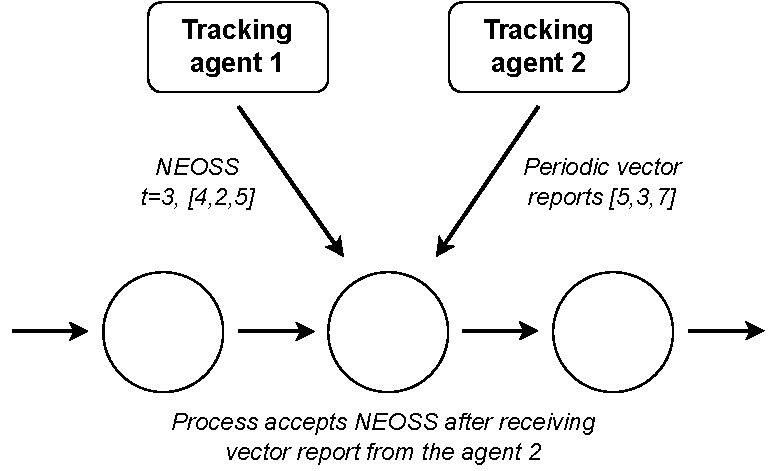
\includegraphics[width=0.6\textwidth]{Chapters/Tracker/pics/distributed-tracker.pdf}
  \caption{Example of a NEOSS and a vector report}
  \label{fig:distributed-tracker}
\end{figure}

In many cases, a process should not wait for NEOSS from other tracking agent shards because it can be confident that other shards do not have stale NEOSS due to periodic observing of their vectors. Figure~\ref{fig:distributed-tracker} illustrates the example of reports from the tracking agents. The NEOSS from the first tracking agent can be accepted if the second tracking agent has already sent a vector report that is component-wise greater than the vector from the NEOSS.

The vector clock introduction increases the service traffic but allows us to eliminate the bottleneck from the system. The service traffic complexity remains unchanged, but the $O$ factor increases. In the experimental section, we will study how significant this increase is.

Despite the fact that distributed tracking agent makes the whole system more scalable, it may affect the performance as we show further. We also demonstrate in the experimental section that it is hard to overload the centralized tracking agent. Therefore, we recommend using the centralized agent unless the cluster configuration is enormous (more than 100 nodes).


\section{Experimental Study}
\label{fs-experiments}
In previous sections, we put several statements out: \tracker\ framework provides low service traffic, low latency between the actual substream termination and termination event receiving, and SPE throughput does not depend on the substream size. In the experimental part of the paper, we will examine these properties on synthetic and real-world examples. 

As a baseline approach, we utilize the punctuations-based method employed in many state-of-the-art stream processing systems such as Flink~\cite{Carbone:2017:SMA:3137765.3137777}, Storm~\cite{apache:storm:state}, Heron~\cite{Kulkarni:2015:THS:2723372.2742788}, IBM Streams~\cite{jacques2016consistent}. To the best of our knowledge, the punctuation framework is the only existing general-purpose substream management technique. 

We have to implement tracking mechanisms on top of a single SPE to compare tracking mechanisms. Otherwise, the performance could be affected by inequalities in serialization, network protocols, etc.  The difficulty here is that the tracking mechanism is usually a core part of an SPE, and its implementation is often optimized. 

We implemented punctuations and \tracker\ techniques on top of \FlameStream~\cite{we2018beyondmr}. It is an open-source Java-based SPE that allows tracking mechanism customization by its design. In~\cite{we2018adbis}, authors demonstrated that the performance of the \FlameStream\ is comparable to state-of-the-art SPE Flink. We have not exploited the system-specific features while implementing substream management methods. We performed all experiments on virtual machines with a dual-core CPU and 4 GB RAM from one of the major cloud providers. 

\begin{figure}[t!]
\centering
% \small
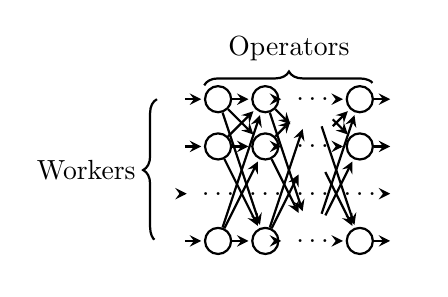
\begin{tikzpicture}[%
  ->, 
  >=stealth,
  shorten >=1pt,
  node distance=0.6cm,
  thick,
  every state/.style={%
  fill=white,
  draw=black,
  text=black
  }   
  ]
    \node[draw, circle] (I_1) [draw=none] {};
    \node[draw, circle] (I_2) [below of=I_1,draw=none] {};
    \node[draw, circle] (I_dots) [below of=I_2,draw=none] {};
    \node[draw, circle] (I_3) [below of=I_dots,draw=none] {};

    \node[draw, circle] (A_1) [right of=I_1] {};
    \node[draw, circle] (A_2) [below of=A_1] {};
    \node[draw, circle] (A_dots) [below of=A_2,draw=none] {$\ldots$};
    \node[draw, circle] (A_3) [below of=A_dots] {};

    \node[draw, circle] (B_1) [right of=A_1] {};
    \node[draw, circle] (B_2) [below of=B_1] {};
    \node[draw, circle] (B_dots) [below of=B_2,draw=none] {$\ldots$};
    \node[draw, circle] (B_3) [below of=B_dots] {};

    \node[draw, circle] (Dots_1) [right of=B_1,draw=none] {$\ldots$};
    \node[draw, circle] (Dots_2) [below of=Dots_1,draw=none] {$\ldots$};
    \node[draw, circle] (Dots_dots) [below of=Dots_2,draw=none] {$\ldots$};
    \node[draw, circle] (Dots_3) [below of=Dots_dots,draw=none] {$\ldots$};

    \node[draw, circle] (Z_1) [right of=Dots_1] {};
    \node[draw, circle] (Z_2) [below of=Z_1] {};
    \node[draw, circle] (Z_dots) [below of=Z_2,draw=none] {$\ldots$};
    \node[draw, circle] (Z_3) [below of=Z_dots] {};

    \node[draw, circle] (O_1) [right of=Z_1,draw=none] {};
    \node[draw, circle] (O_2) [below of=O_1,draw=none] {};
    \node[draw, circle] (O_dots) [below of=O_2,draw=none] {};
    \node[draw, circle] (O_3) [below of=O_dots,draw=none] {};

    \path
          (I_1) edge (A_1)
          (I_2) edge (A_2)
          (I_dots) edge (A_dots)
          (I_3) edge (A_3)
          (A_1) edge (B_1)
          (A_1) edge (B_2)
          (A_1) edge (B_3)
          (A_2) edge (B_1)
          (A_2) edge (B_2)
          (A_2) edge (B_3)
          (A_3) edge (B_1)
          (A_3) edge (B_2)
          (A_3) edge (B_3)
          (B_1) edge (Dots_1)
          (B_1) edge (Dots_2)
          (B_1) edge (Dots_3)
          (B_2) edge (Dots_1)
          (B_2) edge (Dots_2)
          (B_2) edge (Dots_3)
          (B_3) edge (Dots_1)
          (B_3) edge (Dots_2)
          (B_3) edge (Dots_3)
          (Dots_1) edge (Z_1)
          (Dots_1) edge (Z_2)
          (Dots_1) edge (Z_3)
          (Dots_2) edge (Z_1)
          (Dots_2) edge (Z_2)
          (Dots_2) edge (Z_3)
          (Dots_3) edge (Z_1)
          (Dots_3) edge (Z_2)
          (Dots_3) edge (Z_3)
          (Z_1) edge (O_1)
          (Z_2) edge (O_2)
          (Z_dots) edge (O_dots)
          (Z_3) edge (O_3)
          ;
      \draw[-,thick,decorate,decoration={brace,amplitude=5pt,mirror}]
            ([xshift=-5pt]I_1.center) -- ([xshift=-5pt]I_3.center) node[midway, left=4pt] {Workers};
      \draw[-,thick,decorate,decoration={brace,amplitude=5pt}]
            ([xshift=-5pt, yshift=5pt]A_1.center) -- ([xshift=5pt, yshift=5pt]Z_1.center) node[midway, above=5pt] {Operators};
\end{tikzpicture}
\caption{Physical execution graph for experiments} 
\label{fig:physical_graph}
\end{figure}

In the next sections, we will explore our system in four experimental setups:
% \begin{description}
    
    \noindent \textbf{Service traffic:} the last setup aims to demonstrate the asymptotic behavior of competitive approaches. We show that our theoretical estimation meets practical measurements.
    
    \noindent \textbf{Latency:} we explore both the notification latency (a delay between a moment when a substream ends and the reception of the termination event for this substream) and the end-to-end processing latency. We compare the \tracker\ and punctuation approaches on synthetic and real-world workloads in soft and firm bounds.
    
    \noindent \textbf{Maximum SPE throughput:} we study the notification mechanism's influence on the system's maximum throughput using the synthetic workload. This experiment shows an overhead induced by a substream management mechanism on regular data processing.
    
    \noindent \textbf{Substream management for cyclic graphs:} \tracker\ framework supports substream management for cyclic dataflows. In this setup, we demonstrate the benefits of this approach for a novel problem setup: smart caching of operators' states.

% \end{description}

We use a typical synthetic workload shown in Fig.~\ref{fig:physical_graph}. All vertices pass an input element to the next operation. On each step, items are re-partitioned (round-robin). This shape of the physical execution graph allows us to measure the properties of the system with the growth of key switches in a workload. This setup has no computational overhead while covering many realistic scenarios. Graphs with few vertices (under 30) may fit almost any acyclic streaming pipeline~\cite{akidau2018streaming}. Longer instances of this workload correspond to flattened iterative dataflows such as PageRank or Connected Components~\cite{Murray:2013:NTD:2517349.2522738, xu2016efficient}. We reference this synthetic workload as RR-$N$, where $N$ is the number of steps.

\subsection{Service Traffic}
\label{exp_network_traffic}
In the theoretical part of the paper, we put a statement that the service traffic of the \tracker\ grows linearly with the number of processes and granularity of the tracking. In this section, we prove this statement in practice. 

We can measure the extra load provided by tracking mechanisms in the number of service messages sent over the network. In \tracker, there are several types of these messages: SND and RCV reports, NEOSS, and logical clock vectors in the distributed setup. In the baseline approach, all service messages are punctuations. If it is not specified, the graph size is 30, the number of VMs is 15, and the granularity is 10.

% https://gist.github.com/faucct/032aaf6240db361d30a184b1d7bf3c8e
\begin{figure*}[t!]
    \begin{subfigure}[t]{0.3\textwidth}
            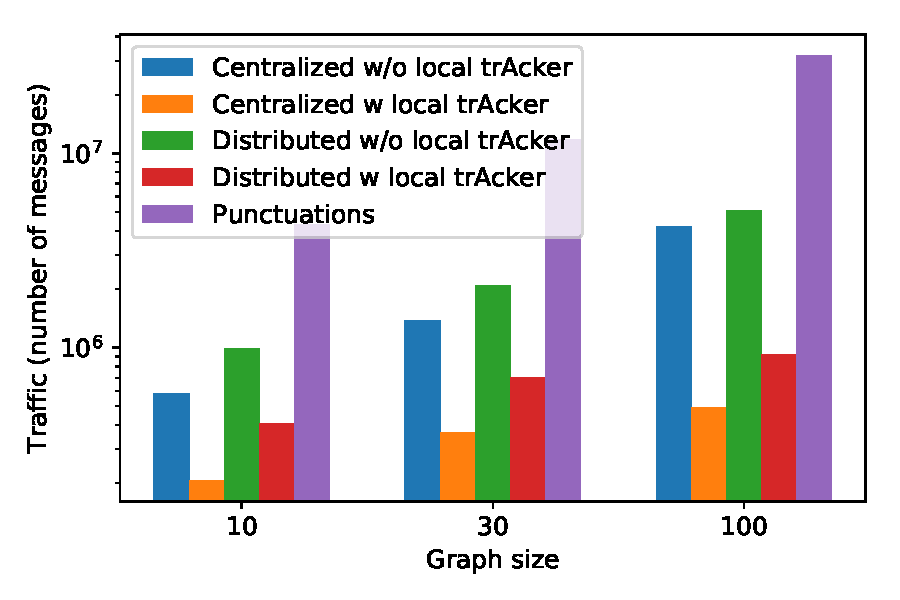
\includegraphics[width=0.99\textwidth]{Chapters/Tracker/pics/traffic_by_graph_size_bars.pdf}
            \caption{Traffic by graph size}
            \label{traffic_graph}
    \end{subfigure}
    \hspace{5mm}
    \begin{subfigure}[t]{0.3\textwidth}
            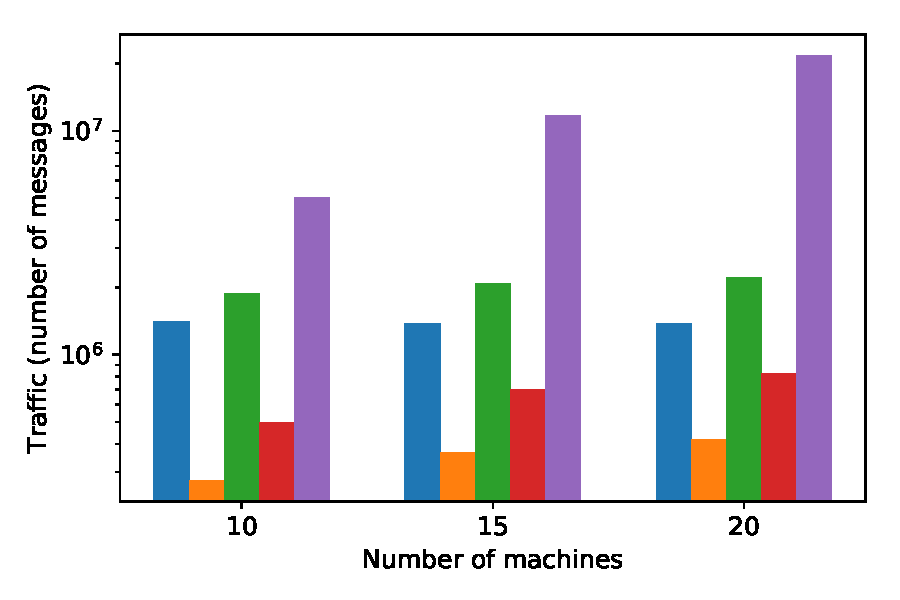
\includegraphics[width=0.99\textwidth]{Chapters/Tracker/pics/traffic_by_number_of_machines_bars.pdf}
            \caption{Traffic by number of VMs}
            \label{traffic_machines}
    \end{subfigure}
    \hspace{5mm}
    \begin{subfigure}[t]{0.3\textwidth}
            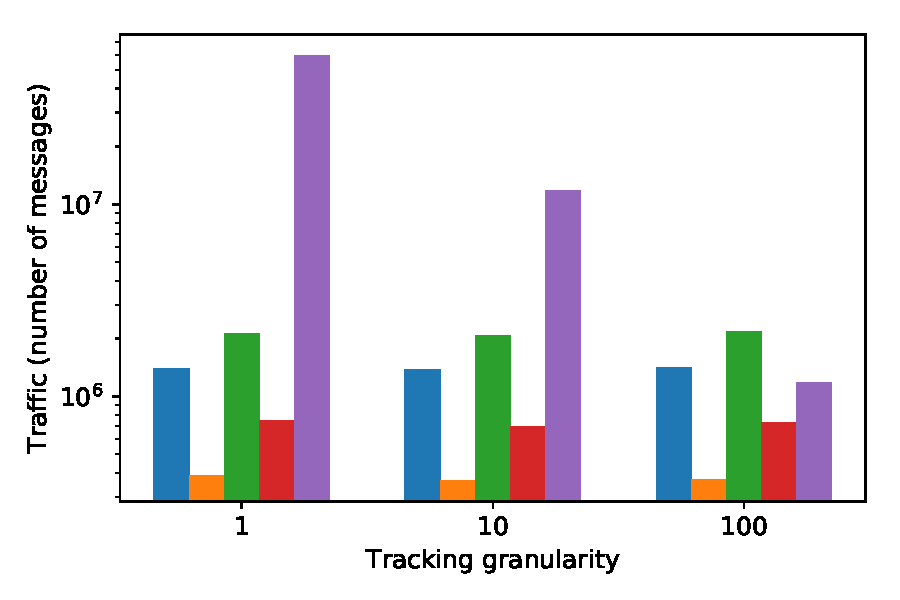
\includegraphics[width=0.99\textwidth]{Chapters/Tracker/pics/traffic_by_tracking_frequency_bars.pdf}
            \caption{Traffic by tracking frequency}
            \label{traffic_granularity}
    \end{subfigure}
    \caption{Service network traffic of punctuations approach and various \tracker\ setups}
    \label{traffic_plots}
\end{figure*}

Figure~\ref{traffic_plots} demonstrates the dependency between service network messages and the size of the logical graph, the number of computational nodes, and the tracking granularity. The extra service traffic is generated by $50K$ input elements sent with 100 items per second arrival rate. 

As shown in Figure~\ref{traffic_graph}, service traffic for punctuations linearly depends on the dataflow size because each new logical vertex adds network broadcasts of punctuations on a physical level. Dependency from the number of computational nodes is quadratic \footnote{At first glance, the dependency may seem linear, but please note that the X-axis covers a range from 10 to 20, and the Y-axis is log-scaled} due to the need to broadcast punctuations to each node after each operator, as Figure~\ref{traffic_machines} demonstrates. 

Figure~\ref{traffic_granularity} indicates that the number of sent service messages for punctuations also directly depends on the tracking granularity. For example, the system should broadcast punctuations after each streaming element in every operator to implement tracking of individual items. 

In the case of \tracker, service traffic depends on the logical graph size and the number of machines because their product forms the number of processes. The growth has a linear trend but can be significantly reduced with the local \tracker\ optimization. Distributed \tracker\ without optimizations provides ~10x less service than punctuations traffic for a graph with 10 vertices and ~30x decrease for a graph with 100 vertices. Regarding the number of machines, the difference is ~10x for 10 nodes and ~30x for 20 nodes. Besides, local \tracker\ optimization allows the system to reduce traffic up to 5 times compared to the straightforward implementation of the distributed \tracker.

% https://gist.github.com/faucct/032aaf6240db361d30a184b1d7bf3c8e
\begin{figure*}[t!]
    \begin{subfigure}[b]{0.3\textwidth}
            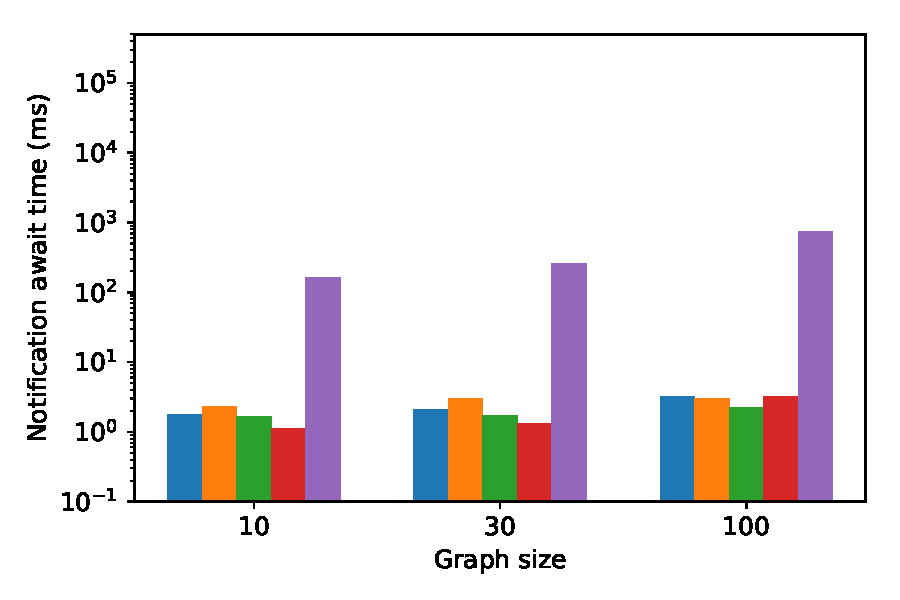
\includegraphics[width=0.99\textwidth]{Chapters/Tracker/pics/notification_await_time_by_graph_size_bars.pdf}
            \caption{Notification latency by graph size}
            \label{notification_graph}
    \end{subfigure}
    \hspace{5mm}
    \begin{subfigure}[b]{0.3\textwidth}
            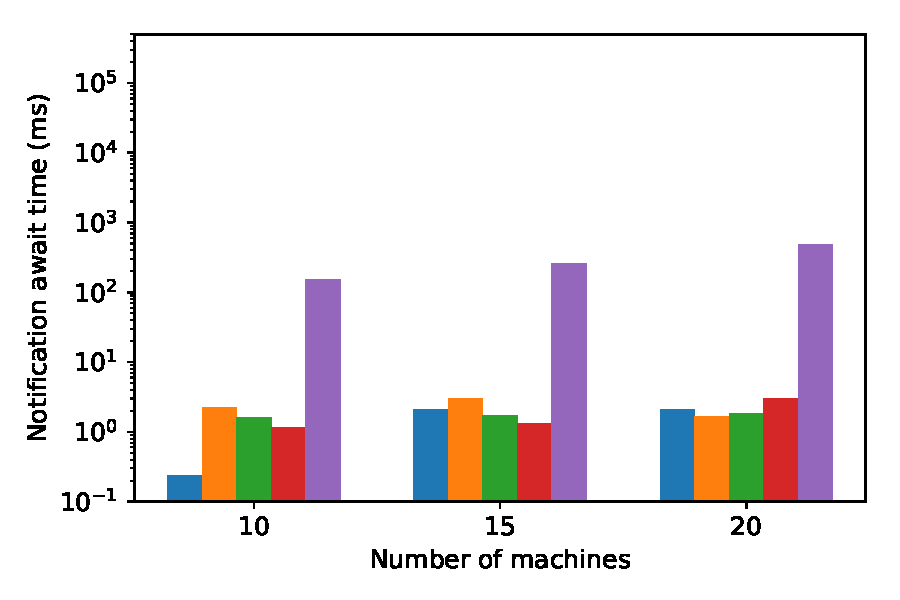
\includegraphics[width=0.99\textwidth]{Chapters/Tracker/pics/notification_await_time_by_number_of_machines_bars.pdf}
            \caption{Notification latency by VMs number}
            \label{notification_machines}
    \end{subfigure}
    \hspace{5mm}
    \begin{subfigure}[b]{0.3\textwidth}
            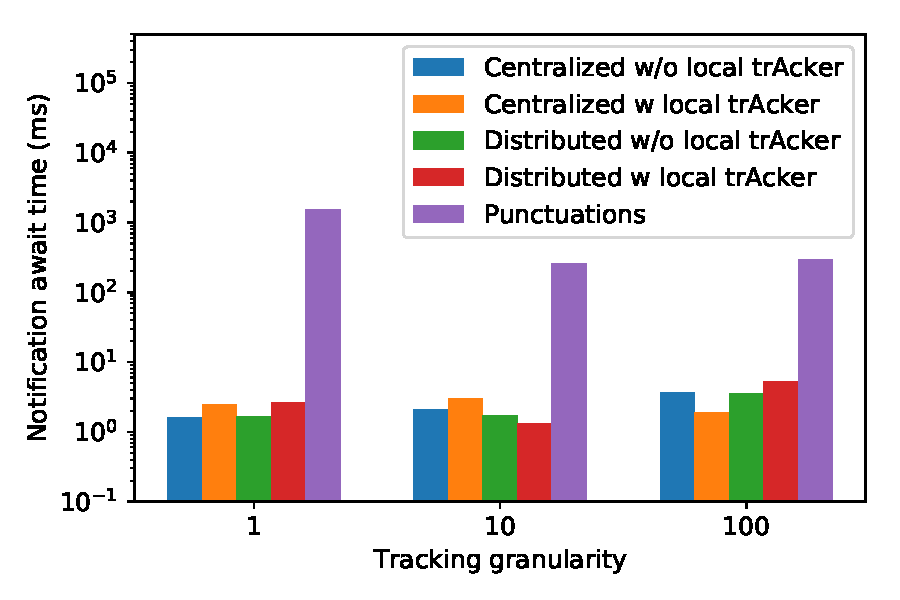
\includegraphics[width=0.99\textwidth]{Chapters/Tracker/pics/notification_await_time_by_tracking_frequency_bars.pdf}
            \caption{Notification latency by granularity}
            \label{notification_granularity}
    \end{subfigure}
    \caption{Notification latency}
    \label{notification_latency}
\end{figure*}

\subsection{Microbenchmarks: Notification Latency}
\label{absolute-latency}

One of the key performance metrics is the latency of notifications: a delay between a moment when a substream ends and the reception of the termination event. This time is added to any operation triggered by termination events~\cite{Carbone:2017:SMA:3137765.3137777, we2018adbis}. For example, Flink finishes its state snapshotting protocol for the epoch (set of input elements) and delivers corresponding output elements to data consumers only after receiving a notification that the whole epoch is completed. We examine end-to-end latency in the next section.

In this experiment, we measure the notification latency as a time interval between a promise from the data source that it will never generate substream elements and the reception of the termination event for this substream. As an experimental workload, we use synthetic workload RR-$N$. We investigate the dependency between the notification latency and cluster sizes, the length $N$ of the workload, and the granularity of tracking (number of elements within a substream). Figure~\ref{notification_latency} shows the results of the experiment. 

The notification latency of a punctuations-based technique depends on the graph and cluster sizes and the granularity of tracking as figures~\ref{notification_graph},\ref{notification_machines}, and~\ref{notification_granularity} indicate. These results align with the overhead induced by punctuations shown in Section~\ref{fs-acker-punctuations}. Notification latency of \tracker\ slightly fluctuates but does not directly depend on the investigated parameters. One can also note that local \tracker\ optimization, as well as distributed version, does not induce heavy overhead on the latency.

The difference in latency between the punctuations and \tracker\ appears because each operator in a dataflow must wait for punctuations from all partitions to sign off the previous operator to send it further to ensure the correctness. 

% https://gist.github.com/faucct/546f5617b958349a125449926373b780
\begin{figure*}[t!]
    \begin{subfigure}[b]{0.30\textwidth}
            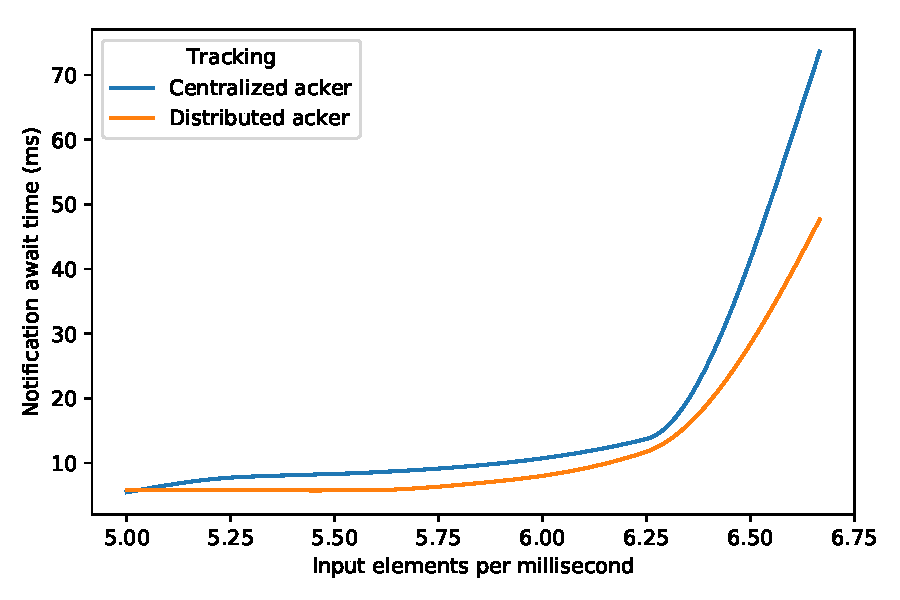
\includegraphics[width=0.99\textwidth]{Chapters/Tracker/pics/scalability_01x.pdf}
            \caption{1x reports}
            \label{1x_acks}
    \end{subfigure}
    \hspace{5mm}
    \begin{subfigure}[b]{0.30\textwidth}
            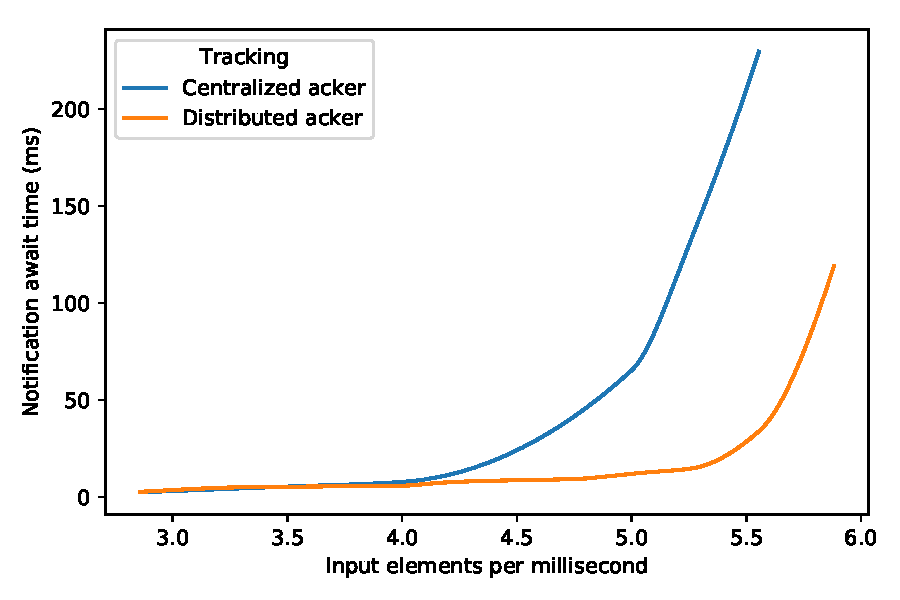
\includegraphics[width=0.99\textwidth]{Chapters/Tracker/pics/scalability_05x.pdf}
            \caption{5x reports}
            \label{5x_acks}
    \end{subfigure}
    \hspace{5mm}
    \begin{subfigure}[b]{0.30\textwidth}
            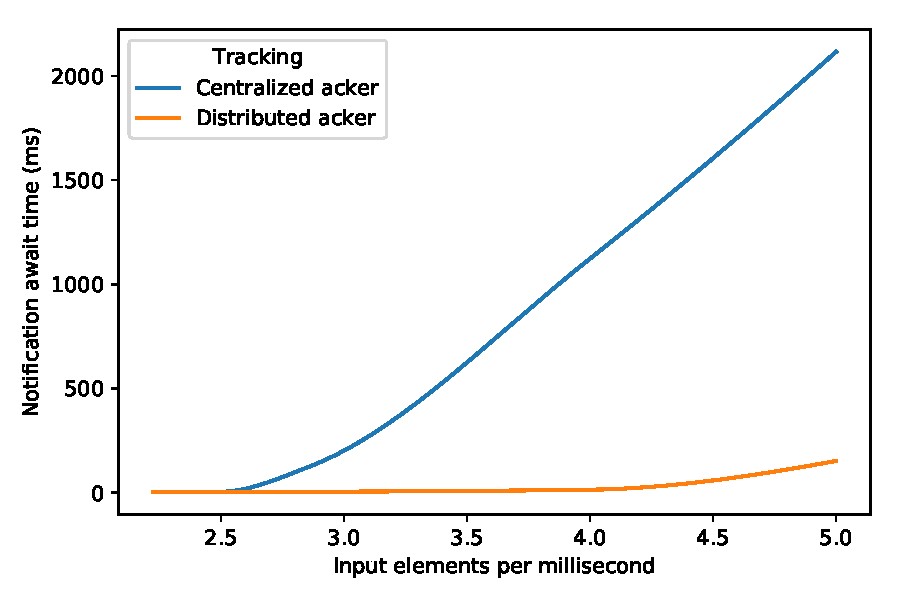
\includegraphics[width=0.99\textwidth]{Chapters/Tracker/pics/scalability_09x.pdf}
            \caption{9x reports}
            \label{9x_acks}
    \end{subfigure}
    \caption{\tracker\ scalability}
    \label{notification_scalability}
\end{figure*}

\subsection{Scalability}

This section demonstrates that the distributed version of the tracking agent allows the substream management mechanism to scale. We measure the median notification latency depending on the rate of input records. The input rate, corresponding to the point where latency starts to grow, indicates a {\em sustainable throughput} of the \tracker. The rapid growth of median latency indicates agent overloading. 

To simulate an additional load on the tracking agent, staying on a budget of 20 machines, we artificially increased the number of sent service messages by 5 and 9 times. We approximate the sustainable throughput by multiplying the extra service messages ratio by the obtained throughput due to the direct dependency between the input and the service message rates. This trick allows us to estimate agent throughput in the number of input data items per second rate without  SPE overloading. Figure~\ref{notification_scalability} demonstrates the results of this experiment.

Without the extra load, distributed tracking agent provides results similar to a centralized setup, as Figure~\ref{1x_acks} indicates. SPE overloading limits the throughput of the agent because it starts to delay sending of service messages. Figure~\ref{5x_acks} demonstrates that with 5x simulated extra load, distributed \tracker\ can sustain $\sim 27K$ requests (items) per second input rate, while centralized provides only $\sim 20K$ RPS throughput. Figure~\ref{9x_acks} shows that with the increase of the extra load to 9x, distributed \tracker\ provides almost 2x throughput increase: $\sim 40K$ RPS against $\sim 22K$ RPS. 

The experiments demonstrate that even the centralized tracking agent can sustain a high input rate within 20 computational nodes. Besides, the distributed version of the agent can make the tracking scalable in larger setups.

\subsection{End-to-end Latency}

In the previous section, we demonstrated that the \tracker\ framework provides lower notification latency than the baseline. In this part, we show how this difference influences end-to-end latency. We use real-world workloads: a window join and a state snapshot. We measure the latency of window join as a duration between the last element of the window entering and the output of window aggregation. We also examine how substream management techniques can affect the duration of taking a state snapshot. In both scenarios, end-to-end latency is directly affected by the notification latency. 

\subsubsection{Window Join}
For the windowed join scenario, we apply the NEXMark benchmark~\cite{tucker2008nexmark} designed to inspect the performance of streaming queries. This benchmark extends the XMark benchmark~\cite{schmidt2002xmark} online auction model, where users can start auctions for items and bid on items. We accept Query 8 from the NEXMark benchmark, defined as follows: {\em Select people who have entered the system and created auctions in the last period}. This query can be implemented using windowed join of persons and auctions. We apply 10 seconds window and 500 RPS per node input rate.

Figure~\ref{fig:nexmark} illustrates the results. The end-to-end latency (a duration between the last element of the window enters the system and the output of window aggregation) within \tracker\ is under 20ms for all setups. In contrast, within punctuations, latency grows up to ~300ms on 30 nodes. After that, it fluctuates slightly. We observe it because the process waits for punctuations from all channels to produce query results. However, with the growth of machines number, the probability that some node delays punctuation increases. After some limit (30 nodes in our case), many nodes delay punctuations, so the latency achieves its maximum. 

\begin{figure*}[t!]
    \begin{subfigure}[b]{0.3\textwidth}
            \includegraphics[width=0.99\textwidth]{Chapters/Tracker/pics/buffering_latencies_barh_100}
            \caption{100 ms snapshot duration}
            \label{100ms_snapshot}
    \end{subfigure}
    \hspace{5mm}
    \begin{subfigure}[b]{0.3\textwidth}
            \includegraphics[width=0.99\textwidth]{Chapters/Tracker/pics/buffering_latencies_barh_500}
            \caption{500 ms snapshot duration}
            \label{500ms_snapshot}
    \end{subfigure}
    \hspace{5mm}
    \begin{subfigure}[b]{0.3\textwidth}
            \includegraphics[width=0.99\textwidth]{Chapters/Tracker/pics/buffering_latencies_barh_1000}
            \caption{1000 ms snapshot duration}
            \label{1000ms_snapshot}
    \end{subfigure}
    \caption{SPE latency spikes during state snapshotting}
    \label{snapshot_spikes}
\end{figure*}

\subsubsection{State Snapshotting}
As mentioned above, state snapshotting is an important application of substream tracking mechanisms. Typically, state snapshotting is implemented as follows: a streaming system divides input records into contiguous substreams called epochs. When an operator entirely processes all items from a particular epoch, it blocks all inputs and persistently saves its local state. Each operator receives the termination event for an epoch and starts to save its state independently from other operators. Flink~\cite{Carbone:2017:SMA:3137765.3137777}, Storm~\cite{apache:storm:state}, IBM Streams~\cite{jacques2016consistent}, and Heron~\cite{Kulkarni:2015:THS:2723372.2742788} implement this state snapshotting scheme. All these systems use punctuation-based techniques to provide notifications for operators.

The punctuation mechanism can imply latency overhead on this protocol. The overhead is caused by blocking an operator after the first punctuation is received until the operator receives punctuations from all inputs. This behavior is known as {\em punctuations alignment} issue~\cite{Carbone:2017:SMA:3137765.3137777}. In the case of \tracker, an operator must buffer elements from the next epoch until the NEOSS for the previous epoch is received.

The local state snapshotting process can be asynchronous in modern SPEs such as Flink~\cite{Carbone:2017:SMA:3137765.3137777}. It implies that local snapshotting duration is unrelated to state size. Nevertheless, the latency of the termination signal for an epoch directly affects the latency of data elements during global state snapshotting because an operator cannot start processing elements from a new epoch until it receives a termination signal for the previous one.

Figure~\ref{snapshot_spikes} demonstrates SPE latency spikes during state snapshotting for punctuations and \tracker, depending on the persistent save duration. In general, \tracker\ provides 50-120 milliseconds fewer latency spikes. This difference can be significant for latency-conscious applications~\cite{zhang2017sub}. The low notification latency explains this difference, as demonstrated in Section~\ref{absolute-latency}. 

\subsection{End-to-end Throughput}
In this experiment, our goal is to find how substream management influences the maximum throughput of an SPE. We measure the median latency of the RR-30 workload using a cluster of 20 nodes, depending on the input rate (input elements per millisecond). The input rate, corresponding to the point where latency starts to grow, indicates a {\em sustainable throughput}~\cite{karimov2018benchmarking}. The growth of median latency indicates system overloading.

Figure~\ref{throughput_overhead} shows that a system without tracking starts to be overloaded at $\sim 9K$ requests (items) per second input rate. The system with the finest-grained centralized \tracker\ setup sustains $\sim 7K$ RPS throughput. Overloading with the punctuations-based approach depends on the tracking granularity: the finest-grained setup does not sustain even $1K$ RPS, while the setup with the granularity of 10 has $\sim 2K$ RPS throughput. Punctuations achieve similar to centralized \tracker\ throughput ($\sim 5K$ RPS) only when injected after each 50 input element.

This experiment shows that punctuations significantly bound the throughput of regular processing within the fine-grained setups. It is explained by the heavy extra network traffic that we demonstrated in Section~\ref{exp_network_traffic}. Note that this additional traffic goes through the same network channels as ordinary data items to ensure that punctuations do not overtake ordinary records. On the other hand, \tracker\ provides less additional system load due to lower extra network usage and exploiting additional network channels.

\begin{figure*}[t!]
    \begin{subfigure}[b]{0.3\textwidth}
            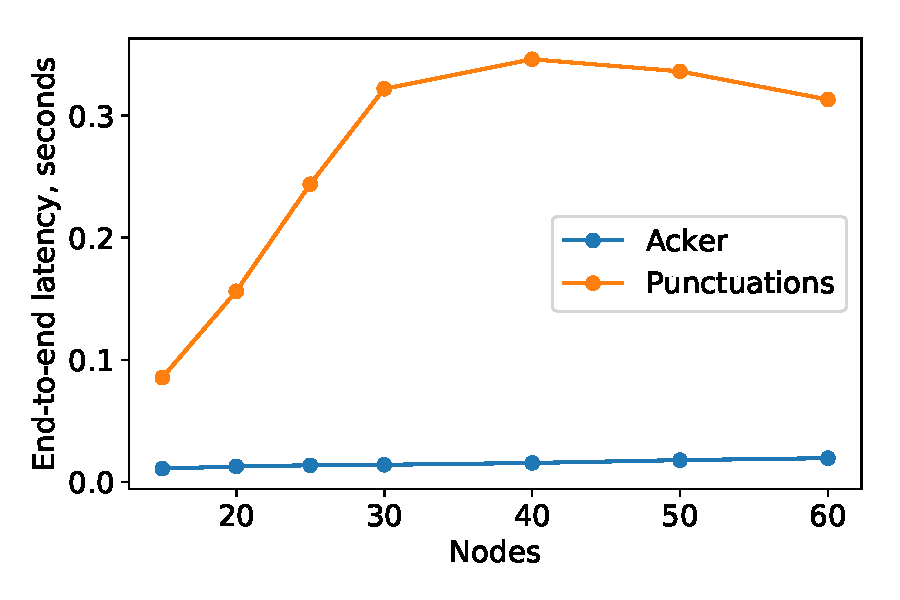
\includegraphics[width=0.99\textwidth]{Chapters/Tracker/pics/nexmark}
            \caption{Nexmark window join scenario}
            \label{fig:nexmark}
    \end{subfigure}
    \hspace{5mm}
    \begin{subfigure}[b]{0.3\textwidth}
            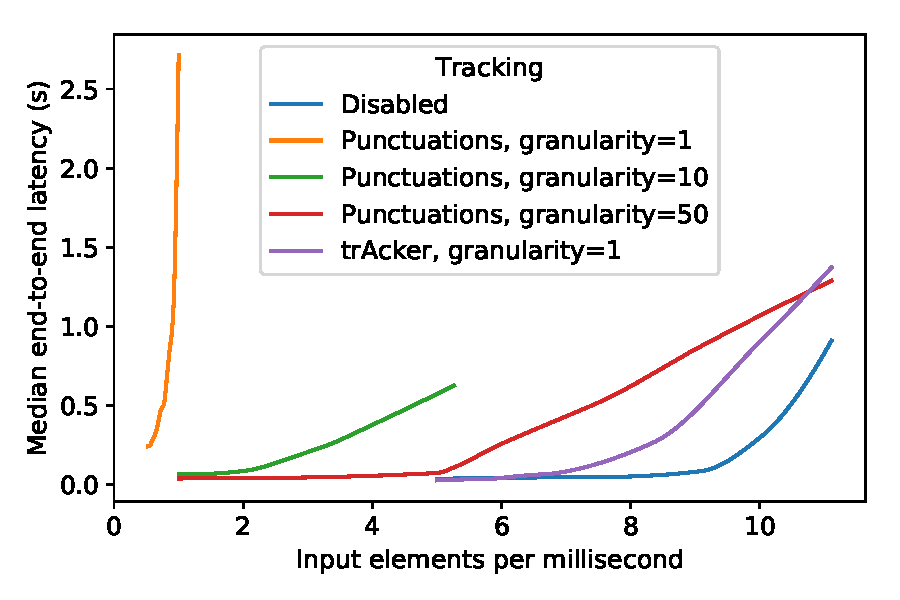
\includegraphics[width=0.99\textwidth]{Chapters/Tracker/pics/throughput_overhead_50}
            \caption{Impact on an SPE throughput}
            \label{throughput_overhead}
    \end{subfigure}
    \hspace{5mm}
    \begin{subfigure}[b]{0.3\textwidth}
            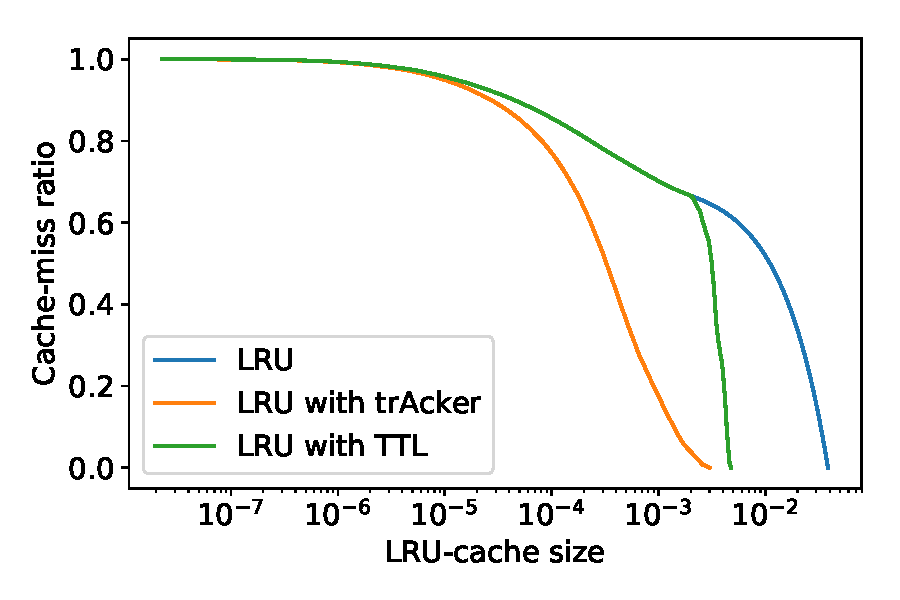
\includegraphics[width=0.99\textwidth]{Chapters/Tracker/pics/dgc_lru_depth_search}
            \caption{State smart cache scenario}
            \label{fig:dgc_lru_depth_search}
    \end{subfigure}
    \caption{Real-world scenarios and maximum throughput}
    \label{various_experiments}
\end{figure*}

\subsection{Substream Management for Cyclic Graphs}

One more practical application of substream tracking is in-memory state optimization. In practice, we often use short-life keys such as session-id, cart-id, or a subset of a wide variety of keys, such as users of social networks. The state associated with such keys should be removed from the memory once the key becomes obsolete. We refer to this task as \textit{distributed garbage collection}.

Substream management can be used to solve this task because we can consider elements bearing a specific key as a substream. In this experiment, we use a \tracker\ for \textit{distributed garbage collection} and compare this approach to more widespread caching techniques.

In the experimental setting, we solve a depth search problem for a graph of Twitter users. This task is relevant for social recommendation systems and requires both scalability and freshness of the results due to the dynamic nature of the graph and the number of nodes. An SPE is a suitable candidate host for such a solution due to the requirement of low latency (freshness). 

Within this model, the user is the key, and the set of her subscribers is the state associated with the key. A stream of queries of user neighborhoods is issued to the system. A resulting set of unique users is expected in return. The execution graph for the depth search problem is cyclic, so \tracker\ suits this task. 

We compare the \textit{distributed garbage collection} approach with LRU caching for this task. The keys are removed from the hot set as soon as none of the currently processed messages contain a reference for it. We used a ratio of cache misses during processing to measure the effectiveness of the memory management mechanism. 

We used 4 nodes in this experiment and fixed the request per second rate to 20. Figure~\ref{fig:dgc_lru_depth_search} presents the results of this experiment. With the growth of the allocated memory, the cache becomes effective. However, the difference between 
\textit{distributed garbage collection} and LRU (with or without optimal TTL) counts in order of magnitude. We believe this type of task should be resolved with GC instead of caching.


\section{Summary}
\label {fs-tracker-conclusion}
In this chapter, we designed and implemented a new substreams management technique called \tracker\ that does not require injecting service elements directly into the stream. Instead, we mark all data elements with ordered labels and use the distributed agent, which notifies operators that a substream ends. Our approach has the following features:

\begin{itemize}
     \item {\bf Cyclic dataflow support:} the method is suitable for problems that require non-linear executions: graph traversing, iterative algorithms, etc. We evaluated this feature within a real-life problem.
     \item {\bf Low overhead:} we showed that our implementation achieves the lower bound of service traffic overhead. We demonstrated that \tracker\ insignificantly affects the throughput of an SPE in practice.
     \item {\bf Fine-grained substream support:} \tracker\ framework is suitable for substreams consisting of a few elements. This feature is achieved due to low traffic overhead and propagation of notifications through separate network channels.
     \item {\bf Scalability:} extra network traffic from operators can be distributed between multiple nodes. Experiments on synthetic dataflows indicated the practical feasibility of balancing extra traffic.
\end{itemize}

These properties of the \tracker\ framework create a possibility to apply substream management in new applications; as indicated in the experimental section, this includes smart caching of operator state and latency-conscious windowed joins.

Fault tolerance is a limitation of the solution presented in this chapter. SPE should ensure recovery of the \tracker\ agent in case of failures. We are leaving this topic for future work.


\chapter{Conclusion}
\label{thesis-chapter-conclusion}
\lhead{\emph{Conclusion}}
This thesis has made contributions to the field of stream processing, addressing the challenges of consistency in a distributed environment. As demonstrated in Chapter~\ref{thesis-chapter-literature-review}, prior work on this topic has made significant progress, with many ideas being implemented in state-of-the-art Stream Processing Engines (SPEs). In this thesis, we focused on building formal models for the existing problems and identifying areas for improvement using the proposed models.

We developed a formal model for the concept of delivery guarantees. We showed connections between the property of determinism and exactly-once delivery guarantee, demonstrating the potential efficiency in terms of latency of deterministic systems ensuring exactly-once. We proposed {\em drifting state} technique that offers a lightweight and efficient method for ensuring determinism and exactly-once processing. This approach allows us to reduce processing latency significantly, providing an improvement over current industrial solutions.

We have formalized the substream management problem. We demonstrated that the extra traffic for a substream management solution cannot be lower than $O(K||\Pi||)$, where $|\Pi|$ is the number of computational nodes and $K$ is the number of substreams. Our findings show that existing punctuation-based frameworks are far from optimal ($O(K|\Pi|^2)$), prompting us to develop the \tracker\ technique. This new approach meets the lower bound of network traffic overhead and is able to handle cycles and fine-grained substreams, making it suitable for advanced stream processing applications.



%\input{Chapters/Chapter2} % Background Theory 

%\input{Chapters/Chapter3} %%% ----------------------------------------------------------------
%% Thesis.tex -- MAIN FILE (the one that you compile with LaTeX)
%% ---------------------------------------------------------------- 

% Set up the document
\documentclass[a4paper, 12pt, oneside]{Thesis}  % Use the "Thesis" style, based on the ECS Thesis style by Steve Gunn
\graphicspath{Figures/}  % Location of the graphics files (set up for graphics to be in PDF format)

% Include any extra LaTeX packages required
\usepackage[square, numbers, comma, sort&compress]{natbib}  % Use the "Natbib" style for the references in the Bibliography
\usepackage{verbatim}  % Needed for the "comment" environment to make LaTeX comments
\usepackage{vector}  % Allows "\bvec{}" and "\buvec{}" for "blackboard" style bold vectors in maths
\usepackage{enumitem} % for customizing lists
\usepackage{pdfpages}
\hypersetup{urlcolor=blue, colorlinks=true}  % Colours hyperlinks in blue, but this can be distracting if there are many links.
\renewcommand\bibname{References}
\newcommand {\FlameStream} {FlameStream}
\newcommand {\tracker} {trAcker}

%% ----------------------------------------------------------------
\begin{document}
\frontmatter      % Begin Roman style (i, ii, iii, iv...) page numbering

% Set up the Title Page
\title  {Thesis Title}
\authors  {\texorpdfstring
            {\href{your web site or email address}{Author Name}}
            {Author Name}
            }
\addresses  {\groupname\\\deptname\\\univname}  % Do not change this here, instead these must be set in the "Thesis.cls" file, please look through it instead
\date       {\today}
\subject    {}
\keywords   {}

% \maketitle
%% ----------------------------------------------------------------

\setstretch{1.3}  % It is better to have smaller font and larger line spacing than the other way round

% Define the page headers using the FancyHdr package and set up for one-sided printing
\fancyhead{}  % Clears all page headers and footers
\rhead{\thepage}  % Sets the right side header to show the page number
\lhead{}  % Clears the left side page header

\pagestyle{fancy}  % Finally, use the "fancy" page style to implement the FancyHdr headers

%% ----------------------------------------------------------------
% Declaration Page required for the Thesis, your institution may give you a different text to place here
% \Declaration{

% \addtocontents{toc}{\vspace{1em}}  % Add a gap in the Contents, for aesthetics

% I, AUTHOR NAME, declare that this thesis titled, `THESIS TITLE' and the work presented in it are my own. I confirm that:

% \begin{itemize} 
% \item[\tiny{$\blacksquare$}] This work was done wholly or mainly while in candidature for a research degree at this University.
 
% \item[\tiny{$\blacksquare$}] Where any part of this thesis has previously been submitted for a degree or any other qualification at this University or any other institution, this has been clearly stated.
 
% \item[\tiny{$\blacksquare$}] Where I have consulted the published work of others, this is always clearly attributed.
 
% \item[\tiny{$\blacksquare$}] Where I have quoted from the work of others, the source is always given. With the exception of such quotations, this thesis is entirely my own work.
 
% \item[\tiny{$\blacksquare$}] I have acknowledged all main sources of help.
 
% \item[\tiny{$\blacksquare$}] Where the thesis is based on work done by myself jointly with others, I have made clear exactly what was done by others and what I have contributed myself.
% \\
% \end{itemize}
 
 
% Signed:\\
% \rule[1em]{25em}{0.5pt}  % This prints a line for the signature
 
% Date:\\
% \rule[1em]{25em}{0.5pt}  % This prints a line to write the date
% }
% \clearpage  % Declaration ended, now start a new page

%% ----------------------------------------------------------------
% The "Funny Quote Page"
% \pagestyle{empty}  % No headers or footers for the following pages

% \null\vfill
% % Now comes the "Funny Quote", written in italics
% \textit{``Write a funny quote here.''}

% \begin{flushright}
% If the quote is taken from someone, their name goes here
% \end{flushright}

% \vfill\vfill\vfill\vfill\vfill\vfill\null
% \clearpage  % Funny Quote page ended, start a new page
%% ----------------------------------------------------------------

% The Abstract Page
% \addtotoc{Abstract}  % Add the "Abstract" page entry to the Contents
% \abstract{
% \addtocontents{toc}{\vspace{1em}}  % Add a gap in the Contents, for aesthetics

% The Thesis Abstract is written here (and usually kept to just this page). The page is kept centered vertically so can expand into the blank space above the title too\ldots

% }

% \clearpage  % Abstract ended, start a new page
%% ----------------------------------------------------------------

\setstretch{1.3}  % Reset the line-spacing to 1.3 for body text (if it has changed)

% The Acknowledgements page, for thanking everyone
% \acknowledgements{
% \addtocontents{toc}{\vspace{1em}}  % Add a gap in the Contents, for aesthetics

% The acknowledgements and the people to thank go here, don't forget to include your project advisor\ldots

% }
% \clearpage  % End of the Acknowledgements
%% ----------------------------------------------------------------

\pagestyle{fancy}  %The page style headers have been "empty" all this time, now use the "fancy" headers as defined before to bring them back


\includepdf[pages={1},offset=80 -80]{cover_page.pdf}

%% ----------------------------------------------------------------
\lhead{\emph{Contents}}  % Set the left side page header to "Contents"
\tableofcontents  % Write out the Table of Contents

% % ----------------------------------------------------------------
% \lhead{\emph{List of Figures}}  % Set the left side page header to "List if Figures"
% \listoffigures  % Write out the List of Figures

%% ----------------------------------------------------------------
% \lhead{\emph{List of Tables}}  % Set the left side page header to "List of Tables"
% \listoftables  % Write out the List of Tables

%% ----------------------------------------------------------------
% \setstretch{1.5}  % Set the line spacing to 1.5, this makes the following tables easier to read
% \clearpage  % Start a new page
% \lhead{\emph{Abbreviations}}  % Set the left side page header to "Abbreviations"
% \listofsymbols{ll}  % Include a list of Abbreviations (a table of two columns)
% {
% % \textbf{Acronym} & \textbf{W}hat (it) \textbf{S}tands \textbf{F}or \\
% \textbf{LAH} & \textbf{L}ist \textbf{A}bbreviations \textbf{H}ere \\

% }

%% ----------------------------------------------------------------
% \clearpage  % Start a new page
% \lhead{\emph{Physical Constants}}  % Set the left side page header to "Physical Constants"
% \listofconstants{lrcl}  % Include a list of Physical Constants (a four column table)
% {
% % Constant Name & Symbol & = & Constant Value (with units) \\
% Speed of Light & $c$ & $=$ & $2.997\ 924\ 58\times10^{8}\ \mbox{ms}^{-\mbox{s}}$ (exact)\\

% }

%% ----------------------------------------------------------------
% \clearpage  %Start a new page
% \lhead{\emph{Symbols}}  % Set the left side page header to "Symbols"
% \listofnomenclature{lll}  % Include a list of Symbols (a three column table)
% {
% % symbol & name & unit \\
% $a$ & distance & m \\
% $P$ & power & W (Js$^{-1}$) \\
% & & \\ % Gap to separate the Roman symbols from the Greek
% $\omega$ & angular frequency & rads$^{-1}$ \\
% }
%% ----------------------------------------------------------------
% End of the pre-able, contents and lists of things
% Begin the Dedication page

\setstretch{1.3}  % Return the line spacing back to 1.3

% \pagestyle{empty}  % Page style needs to be empty for this page
% \dedicatory{For/Dedicated to/To my\ldots}

% \addtocontents{toc}{\vspace{2em}}  % Add a gap in the Contents, for aesthetics


%% ----------------------------------------------------------------
\mainmatter	  % Begin normal, numeric (1,2,3...) page numbering
\pagestyle{fancy}  % Return the page headers back to the "fancy" style

% Include the chapters of the thesis, as separate files
% Just uncomment the lines as you write the chapters

\chapter{Introduction}

Distributed batch and stream systems address two distinct data processing scenarios. Batch processing deals with pre-collected and stored static datasets, with latency spanning hours or even days~\cite{carbone2015apache, chang2014hawq, sun2023survey}. Conversely, applications requiring short-term personalization, IoT, or network monitoring demand results with high freshness. In these cases, data appears as a continuous, discrete, and potentially infinite stream of items, necessitating the continuous production of freshly updated results~\cite{fragkoulis2024survey, diro2024anomaly}.

This distinction highlights significant challenges in distributed stream processing, particularly the low latency requirement, which brings forth two major issues. Firstly, a stream processing engine (SPE) requires advanced fault tolerance mechanisms to ensure quick recovery and data consistency during failures~\cite{Wang:2019:LSF:3341301.3359653, akidau2015streaming}. Secondly, there is the challenge of continuously producing a results stream during processing. Determining the precise moment when a resulting item is ready for release in a distributed environment can be complex~\cite{Tucker:2003:EPS:776752.776780, DBLP:journals/pvldb/BegoliACHKKMS21}.

While partial solutions have been proposed for these problems, in this thesis, we: 
\begin{itemize}
    \item Design formal models describing the limitations of existing approaches
    \item Search for more efficient techniques based on the obtained theoretical insights
\end{itemize}

\section{Research Methodology and Novelty}

Our first step is to identify the actual challenges. The challenges have been identified throughout preparation of our prior publications~\cite{we2018adbis, trofimov2018consistency, we2018seim, we2018beyondmr, we2019debs, webirte, thepaper, 10.1145/3524860.3539809, trofimov2023bounding}. We briefly discuss them in Section~\ref{thesis-intro-challenges}. The corresponding literature is reviewed in Chapter~\ref{thesis-chapter-literature-review}.

After the identification of challenges, we design a formal model suitable to describe the corresponding domain. This step allows us to theoretically justify the challenges, compare existing approaches, highlight their advantages and limitations, and identify areas for improvement. Chapter~\ref{thesis-chapter-delivery-guarantees} and Chapter~\ref{thesis-chapter-substreams-consistency} are dedicated for such formal insights.

In the third step, we verify whether our theoretical findings align with experimental studies. At this stage, our goal is to develop technical implementations and ensure that our theoretically more optimal approaches are feasible in practice. Chapter~\ref{thesis-chapter-delivery-guarantees} and Chapter~\ref{thesis-chapter-substreams-consistency} cover these findings.

The novelty of this work lies in addressing open challenges and achieving results that surpass the current state-of-the-art. The theoretical models we have designed are more suitable for describing real-life scenarios than existing alternatives. Additionally, our practical approaches and algorithms outperform those found in current research and industry standards. The main contribuitons of this work are briefly outlined in Section~\ref{thesis-intro-contributions}.

\section{Open Challenges Related to Consistency}
\label{thesis-intro-challenges}

We identify two key challenges in achieving consistency in distributed stream processing, which are critical yet difficult to address in both academic and industrial contexts: the lack of formalization and the high overhead of consistency mechanisms. Specifically, we discuss how these challenges arise in the two main types of consistency covered in this thesis: delivery guarantees and substreams consistency.

\subsection{Lack of formalization}

\subsubsection{Delivery guarantees}

Delivery guarantees, such as at-most-once, at-least-once, and exactly-once, define how and when data is delivered and processed in the system~\cite{fragkoulis2024survey, carbone2018scalable, Akidau:2013:MFS:2536222.2536229}. The type of delivery guarantee chosen for a system directly influences how that system handles failures~\cite{zhang2024survey, silvestre2021clonos, wang2021consistency}. In at-most-once, if a failure occurs during processing, the system may not attempt to reprocess the input, leading to potential data loss. In at-least-once, the system ensures no data is lost by reprocessing inputs in case of failures. However, this can lead to duplicate processing and results if the system doesn't track what has already been processed. In exactly-once, the system ensures that every input is processed exactly one time, even in the case of failures.

In state-of-the-art stream processing systems like Flink~\cite{Carbone:2017:SMA:3137765.3137777} and Spark~\cite{Zaharia:2012:DSE:2342763.2342773}, delivery guarantees are primarily defined through each system's internal failure recovery mechanisms. However, a significant limitation of this approach is the variation in features provided by different recovery mechanisms, complicating the assurance of delivery guarantees across systems. For instance, in Flink with declared at-least-once guarantee, if an operation within the execution graph is non-commutative, this can result not only in duplicated outputs but also in outputs that are inconsistent with previously released data, as we will further demonstrate in this thesis. Consequently, one of the critical issues we have identified is the poor formalization of delivery guarantees. A deeper understanding of the expected outputs following a system failure is essential for developing reliable, production-ready systems based on distributed stream processing.

\subsubsection{Substreams consistency}

There are plenty of data processing scenarios where results are most valuable at the time of data arrival, for example, IoT, news processing, financial analysis, fraud detection, and network monitoring. However, regular blocking data processing operators read an entire input before producing an output and can never release a result in the case of a stream. To handle this problem, one can divide the whole unbounded, potentially infinite data stream into bounded, possibly overlapping substreams˜\cite{tucker2003exploiting}. In this case, an operator can produce an output when a corresponding substream terminates.

Generating a substream termination event is a challenging task that often depends on the specific properties of practical problems. For instance, a deterministic windowed join operation\footnote{given the identical sequences of input tuples, the identical output tuples will be produced} requires that the order of termination signals mirrors the order of input elements (termination events from data producers)~\cite{najdataei2019stretch, gulisano2016scalejoin}. Another example is an epoch: a substream that an SPE should process atomically. A termination event for an epoch must occur before any elements of the subsequent epoch arrive. These examples demonstrate that it is crucial to formally define the properties of substream management techniques to determine their suitability for specific scenarios.

\subsection{High overhead on consistency mechanisms that leads to high processing latency}

\subsubsection{Delivery guarantees}

One of the most challenging tasks for streaming systems is to design and implement delivery guarantees. 
Streaming systems must release output elements before processing has finished because the input data is assumed to be unbounded. Exactly-once is the strongest and the most valuable guarantee from the user perspective as it ensures that input elements are processed atomically and are not lost. These notions are seemingly simple but shadow the dependency of an output item on the {\em system state} as well as on the input item. 
Streaming systems face the need to recover computations consistently with previous input data, current system state, and already delivered elements.
This requirement makes failure recovery mechanisms somewhat complicated. 

This complication is resolved by most existing stream processing engines. 
Flink ensures the atomicity of state updates and delivery using a protocol based on distributed transactions. 
Google MillWheel~\cite{Akidau:2013:MFS:2536222.2536229} enforces consistency between state and output elements by writing the results of each operation to persistent external storage. 
Micro-batching engines like Storm Trident~\cite{apache:storm:trident} and Spark Streaming~\cite{Zaharia:2012:DSE:2342763.2342773} process data in small-sized blocks. 
Each block is atomically processed at each stage of a data flow, providing properties similar to batch processing. 
The price for exactly-once delivery is a high latency observed in these implementations (e.g., ~\cite{7530084, 7474816}). It is unclear if it is possible to mitigate the latency overhead on exactly-once enforcement.

\subsubsection{Substreams consistency}

A popular method for the generation of substream termination events is the punctuation framework~\cite{tucker2003exploiting} applied in many production-scale SPEs such as Flink~\cite{carbone2015apache}, Heron~\cite{Kulkarni:2015:THS:2723372.2742788}, Samza~\cite{Noghabi:2017:SSS:3137765.3137770}, IBM Streams~\cite{jacques2016consistent}, Apex~\cite{pathak2016introduction}. The main idea behind this framework is to divide the stream by injecting special elements called {\em punctuations} that define substreams ``borders''. An SPE propagates these special elements via the same network channels as data elements. The high network overhead is one of the major limitations of the punctuation framework. Network traffic complexity for this method is $O(K|\Pi|^2)$, where $|\Pi|$ is the number of processes and $K$ is the number of substreams because each process should propagate punctuations to all output channels. The above formula estimates the number of punctuation messages needed in the worst case of fully interconnected processes. 

We argue that the worst case can appear on any execution graph that contains a re-partitioning operator. Indeed, SPEs try to distribute workload evenly between processes~\cite{carbone2015apache, Kulkarni:2015:THS:2723372.2742788, Akidau:2013:MFS:2536222.2536229}, so elements of a substream can be evenly distributed among processes as well. When a process reaches the end of a substream, it must broadcast the punctuation because the items of the part of a sub-stream handled by this process are re-distributed evenly for subsequent processing. Substreams can be {\em fine-grained}: for example, each user session defines a substream. If there are a lot of small substreams, an inefficient substreaming system can degrade the latency~\cite{DBLP:journals/pvldb/BegoliACHKKMS21} and the throughput of an SPE~\cite{Li:2008:OPN:1453856.1453890} or affect the performance of state checkpointing~\cite{zhang2021research}. Therefore, reducing an overhead on substreams management is an important open challenge in distributed stream processing.

\section{Primary Contributions}
\label{thesis-intro-contributions}

We highlight the main results of this work in the following contributions, which address the challenges detailed in Section~\ref{thesis-intro-challenges}.

\subsection{Delivery guarantees formalization}

We introduced a formal framework for modeling consistency properties for any stream processing system~\cite{thepaper}. It was shown that the property of determinism is tightly connected with the concept of exactly-once. We proved that non-deterministic systems must persistently save a state of non-commutative operations before output delivery in order to achieve exactly-once.

We demonstrated that most of the state-of-the-art stream processing systems~\cite{Carbone:2017:SMA:3137765.3137777, Zaharia:2012:DSE:2342763.2342773, Akidau:2013:MFS:2536222.2536229, apache:storm:trident} use one of the following approaches to overcome this problem: 

\begin{itemize}
    \item Inherit exactly-once from batch processing using small-sized batches (micro-batching)
    \item Apply distributed transaction control protocols which guarantee that states are saved before delivery of elements affected by these states
    \item Write results of an operation to external storage on each input element
\end{itemize}

All these methods experience difficulties with working under low-latency requirements (less than a second). In the first case, latency cannot be lower than the batching period, in the second case, the distributed two-phase commit may result in a significant increase of latency, while in the third case latency is bounded below by the duration of external writes. The formal framework along with the mentioned theoretical insights are covered in Chapter~\ref{thesis-chapter-delivery-guarantees}.

\subsection{Exactly-once based on lightweight determinism}

Using our formal inference, we designed the \textit{drifting state} technique~\cite{we2018adbis}, a lightweight optimistic approach for ensuring deterministic processing. As demonstrated earlier, deterministic systems can theoretically be more efficient for exactly-once processing in terms of latency, so that we adapted drifting state to achieve exactly-once guarantee~\cite{thepaper}. Our protocols offer several important features:

\begin{itemize}
    \item Elements are processed in a pure streaming fashion, without the need for input buffering.
    \item Business-logic computations, state snapshotting, and the delivery of output items operate asynchronously and independently.
    \item Exactly-once processing semantics are maintained.
\end{itemize}

We implemented the prototype of the proposed technique to examine its performance~\cite{we2018adbis, we2018seim, thepaper}. Our experiments demonstrated that the introduced protocols for fault tolerance are scalable and provide remarkably low overhead within different computational layouts. The comparison with the industrial stream processing solution indicated that our prototype could provide lower latency under exactly-once requirement. The drifting state technique along with exactly-once implementation on top of it and experimental study are detailed in Chapter~\ref{thesis-chapther-optimistic}.

\subsection{Formalization of substreams consistency}

We formalized the problem of substreams management and highlighted its main features~\cite{10.1145/3524860.3539809, trofimov2023bounding}. Particularly, we introduced the notions of {\em soft bound} and {\em firm bound} required by various stream processing scenarios. Some applications that apply substream management systems do not require any particular properties of termination events. In this case, we denote the guarantee provided by such events as {\em soft bound} because termination events indicate that the substream ended some time ago. However, other problems require a {\em firm bound}: guarantee that the substream ends {\em exactly} after the termination event. For example, a commonly used snapshotting protocol~\cite{2015arXiv150608603C, jacques2016consistent} relies on an {\em epoch}. An epoch is a special substream that must be processed atomically. Therefore, the SPE requires the termination event for a given epoch to occur immediately after the last processing event belonging to that epoch. Otherwise, the snapshot can be inconsistent, capturing elements from multiple epochs.

We also provided several insights into the performance of substream management systems. We showed that the network overhead induced by a substream management system cannot be lower than linear in terms of the number of computational nodes. We demonstrated that the state-of-the-art punctuations framework, as applied in many production-scale SPEs~\cite{tucker2003exploiting}, incurs quadratic network overhead with respect to the number of computational nodes, indicating that it is far from the lower bound. Chapter~\ref{thesis-chapter-substreams-consistency} is dedicated to the substreams formal model and the mentioned performance insights.

\subsection{Substream management approach reaching lower bound of network traffic overhead}

We designed and implemented a new substreams management technique called \tracker~\cite{10.1145/3524860.3539809, trofimov2023bounding}. Our approach has the following features:

\begin{itemize}
    \item Efficiency due to the lower bound of service traffic overhead
    \item Suitability for problems that require non-linear executions: graph traversing, iterative algorithms, etc.
    \item Suitability for substreams consisting of a few elements
    \item Scalability due to the distribution of extra network traffic from operators between multiple nodes
\end{itemize}

These properties of the \tracker\ framework create a possibility to apply substream management in new applications; this includes smart caching of operator state and latency-conscious windowed joins.

We also demonstrated that \tracker\ outperforms state-of-the-art substream management mechanisms in real-life scenarios. The design of the \tracker\ framework along with its implementation details and experimental study are discussed in Chapter~\ref{thesis-chapter-tracker}.

\section{Published Work}

Most of the material in this dissertation is derived from work that has already been published and peer-reviewed. Particularly, Chapter~\ref{thesis-chapter-delivery-guarantees} and Chapter~\ref{thesis-chapther-optimistic} include content from papers on optimistic technique for achieving determinism and the exactly-once approach on top of that~\cite{we2018seim, we2018adbis, thepaper, we2018beyondmr, trofimov2018consistency, webirte, we2019debs}. Chapter~\ref{thesis-chapter-substreams-consistency} and Chapter~\ref{thesis-chapter-tracker} are based on papers on \tracker\ framework and substream management~\cite{10.1145/3524860.3539809, trofimov2023bounding}.

The complete list of published material along with assigned contributions is the following:

\begin{enumerate}
    \item Artem Trofimov, Nikita Sokolov, Nikita Marshalkin, Igor Kuralenok, and Boris Novikov. \textbf{Bounding substreams in distributed stream processing}. Information Systems, Volume 117, 2023. \newline
    
    \textit{Contribution:} The author of this dissertation co-designed a substream management framework and a formal model for the substream management domain as well as leading the writing of the paper.

    \item Artem Trofimov, Nikita Sokolov, Nikita Marshalkin, Igor Kuralenok, and Boris Novikov. \textbf{Substream management in distributed streaming dataflows}. In Proceedings of the 16th ACM International Conference on Distributed and Event-Based Systems (DEBS '22), pp. 55-66. ACM, 2022. \newline
    
    \textit{Contribution:} The author of this dissertation co-designed a substream management framework and a formal model for the substream management domain as well as leading the writing of the paper.

    \item Igor Kuralenok, Artem Trofimov, Nikita Marshalkin, and Boris Novikov. \textbf{Deterministic Model for Distributed Speculative Stream Processing}. In European Conference on Advances in Databases and Information Systems (pp. 233-246). Cham: Springer International Publishing, 2018. \newline
    
    \textit{Contribution:} The author of this dissertation co-designed mechanism for ensuring determinism, performed the experiments, and co-authored the paper.

    \item Igor Kuralenok, Nikita Marshalkin, Artem Trofimov, and Boris Novikov. \textbf{An optimistic approach to handle out-of-order events within analytical stream processing}. In Third Conference on Software Engineering and Information Management (SEIM-2018) (pp. 22-29), 2018. \newline
    
    \textit{Contribution:} The author of this dissertation co-implemented mechanism for handling out-of-order elements, performed the experiments, and co-authored the paper.

    \item Artem Trofimov, Igor Kuralenok, Nikita Marshalkin, and Boris Novikov. \textbf{Delivery, consistency, and determinism: rethinking guarantees in distributed stream processing}. arXiv preprint arXiv:1907.06250, 2019. \newline
    
    \textit{Contribution:} The author of this dissertation co-designed a formal model for delivery guarantees and a mechanism for achieving exactly-once as well as leading the writing of the paper.

    \item Artem Trofimov, Nikita Sokolov, Mikhail Shavkunov, Igor Kuralenok, and Boris Novikov. \textbf{Distributed Classification of Text Streams: Limitations, Challenges, and Solutions}. In Proceedings of Real-Time Business Intelligence and Analytics (pp. 1-6), 2019. \newline
    
    \textit{Contribution:} The author of this dissertation performed experiments and led the writing of the paper.

    \item Artem Trofimov. \textbf{Consistency Maintenance in Distributed Analytical Stream Processing}. In New Trends in Databases and Information Systems: ADBIS 2018 Short Papers and Workshops, AI* QA, BIGPMED, CSACDB, M2U, BigDataMAPS, ISTREND, DC, Budapest, Hungary, September, 2-5, 2018, Proceedings 22. Springer International Publishing, 2018. \newline
    
    \textit{Contribution:} The author of this dissertation led the writing of the paper.

    \item Igor Kuralenok, Artem Trofimov, Nikita Marshalkin, and Boris Novikov. \textbf{Flamestream: model and runtime for distributed stream processing}. In Proceedings of the 5th ACM SIGMOD Workshop on Algorithms and Systems for MapReduce and Beyond (pp. 1-2), 2018 \newline
    
    \textit{Contribution:} The author of this dissertation performed experiments and co-authored the paper.

    \item Artem Trofimov, Mikhail Shavkunov, Sergey Reznick, Nikita Sokolov, Mikhail Yutman, Igor Kuralenok, and Boris Novikov. \textbf{Reproducible and reliable distributed classification of text streams}. In Proceedings of the 13th ACM International Conference on Distributed and Event-based Systems (pp. 264-265), 2019. \newline
    
    \textit{Contribution:} The author of this dissertation led the writing of the paper.
\end{enumerate}

\section{Dissertation Outline}
 % Introduction

\chapter{Consistency and Fault Tolerance in Distributed Stream Processing}
\label{thesis-chapter-literature-review}
\lhead{\emph{Consistency and Fault Tolerance in Distributed Stream Processing}}

\section{Consistency in distributed stream processing}
\label{consistency_overview}

In this section, we discuss several types of consistency in distributed stream processing. We start with delivery guarantees in Section~\ref{delivery_guarantees}: exactly-once, at-least-once, and at-most-once. Delivery guarantees specify the rules for how a system should behave in case of node failures to maintain a consistent state and prevent data loss or duplication.

Section~\ref{completeness} covers the completeness of results.  In a distributed system, especially in streaming, data can arrive out of order, be delayed, or even temporarily lost. Completeness guarantees that the system's output reflects all the data that should have been processed within a given window or time frame, preventing partial or misleading results.

Eventually, in Section~\ref{transactional} we discuss transactional stream processing (TSP). TSP integrates the low latency processing capabilities of stream processing with the reliability and consistency guarantees of traditional transactional systems. TSP systems achieve consistency by incorporating the ACID (Atomicity, Consistency, Isolation, Durability) properties typically found in traditional database transactions.

% Eventually, in Section~\ref{statistical} we touch on the topic of statistical consistency in stream processing. Statistical consistency refers to the accuracy and reliability of statistical estimates and summaries derived from continuous data streams. This type of consistency ensures that the statistical measures calculated over the data stream are accurate and close to the expected values. Statistical consistency is close to anomaly detection because anomalies, such as sudden spikes or unusual data patterns, can be detected based on deviations from these consistent statistical measures.

\subsection{Delivery guarantees}
\label{delivery_guarantees}

\subsubsection{Types of delivery guarantees}

Delivery guarantees, such as at-most-once, at-least-once, and exactly-once, define how and when data is delivered and processed in the system~\cite{fragkoulis2024survey, carbone2018scalable, Akidau:2013:MFS:2536222.2536229}:
\begin{itemize}
    \item At-most-once is a delivery guarantee in system processing where an input element is processed atomically (with all its derivatives) or not processed at all. This means that the system ensures that each input element is processed only one time at maximum, but there's a possibility that some input elements may not get processed.
    \item At-least-once is a type of delivery guarantee where the system ensures that every input element is processed one or more times. This could lead to potential duplication if an input contains duplicated items. This method ensures no data is lost, but it does not prevent possible repetitions.
    \item Exactly-once is a system processing term that guarantees each input element or transaction is processed exactly one time. This means that it ensures there is no data loss and no duplicate processing. It combines both the prevention of input data losses and the avoidance of repeated delivery of results.
\end{itemize}

The type of delivery guarantee chosen for a system directly influences how that system handles failures~\cite{zhang2024survey, silvestre2021clonos, wang2021consistency}. In at-most-once delivery, if a failure occurs during processing, the system may not attempt to reprocess the input, leading to potential data loss. In at-least-once delivery, the system ensures no data is lost by reprocessing inputs in case of failures. However, this can lead to duplicate processing and results if the system doesn't track what has already been processed. In exactly-once delivery, the system ensures that every input is processed exactly one time, even in the case of failures. This is the most complex to implement as it needs to ensure atomicity between reading input data, processing, and delivering results, and it requires the system to be able to recover to a consistent state after a failure~\cite{Carbone:2017:SMA:3137765.3137777}.

\subsubsection{State recovery and consistency}

State recovery is crucial for consistency because it allows a system to return to a known, correct state after a failure. Without state recovery, a failure can leave the system in an inconsistent state, where the results of some operations are lost or incorrect~\cite{Carbone:2017:SMA:3137765.3137777, Akidau:2013:MFS:2536222.2536229}. State recovery also allows the system to resume processing from a recent checkpoint instead of starting over from the beginning, saving both time and computational resources.

In the context of data processing systems, state recovery is particularly important for handling transient failures. For instance, if a node in a distributed system fails and then restarts, it needs to know what data it has already processed to avoid duplicating work or missing some data. By restoring its state from before the failure, the node can ensure it processes each piece of data exactly once, maintaining the consistency of the system's output~\cite{silvestre2021clonos, Carbone:2017:SMA:3137765.3137777, wang2021consistency}.

The two main ways to recover a consistent state are~\cite{fragkoulis2024survey, zhang2024survey}:

\begin{enumerate}
    \item {\em Global State Snapshotting} involves taking snapshots of the entire system's state at given points in time. The snapshot includes the state of all nodes in the system and any in-transit messages. This approach provides a consistent view of the system, but it may lead to high overhead on recovery because there is a need to re-process all data items since the previous snapshot is taken.
    \item {\em Record-Level Logging} involves saving data elements, state, or causal logs after processing each record or a batch of records. This allows for very fine-grained recovery, as the system can resume processing from the last processed record. However, this approach can introduce significant overhead, as the system needs to save the state frequently.
\end{enumerate}

We will dive into the details of the specific state recovery techniques in Section~\ref{phd-related-fault-tolerance}.

\subsubsection{Suitable consistency levels for various types of problems}

Distributed stream processing is used in many areas~\cite{fragkoulis2024survey} including network monitoring, IoT, financial processing, machine learning, etc. There are many applications, such as financial systems, where the integrity and correctness of the data are crucial~\cite{zhang2024survey}. Therefore, such applications usually require exactly-once delivery guarantee. In applications like fraud detection, IoT, earthquakes detection, or network security, where each piece of data needs to be analyzed to detect potential anomalies or threats, exactly-once processing is also critical. Missing a data point or processing it multiple times could lead to failure in detecting an anomaly or false alarms~\cite{zhou2019scalable, diro2024anomaly, 10.1093/gji/ggac355, geldenhuys2021dependable}.

On the other hand, the need for exactly-once processing guarantees in machine learning applications depends on the specific requirements of the problem being addressed. While exactly-once processing is critical in some scenarios to ensure data integrity and correctness, it might be less crucial in others~\cite{boden2017distributed, webirte}:
\begin{itemize}
    \item {\em Training Data Preparation}: In the preparation phase of training data, ensuring that each data sample is included exactly once is important for the accuracy of the model. Duplicate data can skew the distribution of the training set, leading to biased models. However, many machine learning algorithms are robust to small inconsistencies, so exactly-once processing might not always be strictly required.
    \item {\em Model Training}: During the training process, especially in distributed systems, exactly-once processing might be less critical depending on the training algorithm. For example, stochastic gradient descent, commonly used in training neural networks, can inherently tolerate some level of noise and inconsistency in data updates, as it is designed to converge despite the random nature of the input data batches.
    \item {\em Real-time Predictions}: For real-time machine learning systems, such as those used in recommendation engines or dynamic pricing models, exactly-once processing can be crucial. Ensuring that each event or piece of data affects the system once prevents the model from making decisions based on duplicated data, which could mislead the prediction outcomes.
    \item {\em Online Learning}: In online learning, where the model continuously updates itself based on incoming data streams, exactly-once processing is beneficial to maintain the correctness of the model updates. Duplicate or missed data points can significantly affect the accuracy and reliability.
\end{itemize}

In summary, whether exactly-once or at-least-once processing is required primarily depends on the tolerance of the specific algorithm to inconsistencies and the impact of data duplication or loss on the application effectiveness. In cases where data integrity directly influences decision-making processes, exactly-once processing becomes more crucial.

\subsection{Completeness of results}
\label{completeness}

In static batch data processing, an operator can read an entire input and produce an output. However, with unbounded streams, there is no defined end to the data, which means that the traditional approach of processing all the data before generating an output is not feasible. Therefore, another important aspect of consistency in distributed stream processing is the {\em completeness} of results~\cite{Tucker:2003:EPS:776752.776780}. Completeness of results in stream processing refers to the extent to which the results generated from processing a data stream fully and accurately reflect all the relevant data for a given query or operation. In other words, it measures whether all the necessary data points have been included in the computation to produce a correct and comprehensive result~\cite{akidau2015streaming}.

\subsubsection{Substreams}

Substreams in stream processing refer to smaller, finite segments or partitions of a larger, potentially infinite data stream~\cite{Tucker:2003:EPS:776752.776780}. Substreams are created to manage and process data more efficiently by breaking down the continuous data flow into more manageable chunks. A substream can be expressed as a predicate on stream elements. All elements satisfying the predicate form the substream.

For example, in a stream of web server logs, one could create substreams for each user session, where each substream contains all events (page views, clicks, etc.) that occurred within a specific session. Another example is the system that analyzes customers' activity within hourly windows. It needs to ensure that all orders within that hour are included in the analysis. In this case, the substream is formed by all events from that window.

Substreams allow outputting results before all input is processed. By dividing the continuous data stream into smaller, manageable segments, an SPE can produce intermediate results as each substream is processed. In terms of substreams, the problem of result completeness comes down to ensuring that all substream elements are processed before outputting the corresponding result. 

\subsubsection{Detecting termination of substreams}

Solving the problem of detecting that all substream elements have been processed is the prerequisite for ensuring that system results are complete. The strict substream termination guarantee consists of two parts: the source must promise that no more messages from the substream may emerge, and the system must ensure it contains no substream messages. 

The first task requires a contract with a particular data source and is discussed further in this section. Promises, that are also called {\em watermarks}, can be generated periodically or heuristic-based~\cite{Akidau:2013:MFS:2536222.2536229, akidau2015streaming}. There are adaptive approaches to generating watermarks. The first one treats change in the skewness between the event time and processing time of stream elements as a concept drift~\cite{awad2019adaptive}. It utilizes the adaptive window (ADWIN) drift detection technique~\cite{bifet2007learning, grulich2018scalable} to determine when and with what value to generate a new watermark. Another adaptive watermark generation mechanism leverages a time series prediction model. This mechanism dynamically adjusts the frequency and timing of watermark distribution based on the ratio of disordered data and other lateness properties of the data stream~\cite{song2021adaptive}.

The second task is also challenging due to the distributed nature of the system and the absence of a standard message lifetime limit. Hence, there is a need for a more complex mechanism than checking that all elements arrived in a strict order~\cite{Li:2008:OPN:1453856.1453890}. This difficulty increases with the introduction of cycles into dataflow. Punctuations framework was firstly introduced in~\cite{Tucker:2003:EPS:776752.776780} and then developed to a distributed setup in~\cite{Akidau:2015:DMP:2824032.2824076} and~\cite{Carbone:2017:SMA:3137765.3137777}. According to this method, special data elements, called punctuations, are injected into the data stream. These punctuations serve as markers that define the boundaries of substreams. They indicate that all elements following punctuation will not satisfy a specified predicate, effectively marking the end of the corresponding substream. While the punctuations framework is widely adopted in major SPEs~\cite{carbone2015apache, Noghabi:2017:SSS:3137765.3137770, Kulkarni:2015:THS:2723372.2742788}, it has several pitfalls. It is not applicable for execution graphs with cycles~\cite{carbone2018scalable}. Additionally, the punctuations framework generates extra service traffic that can degrade the latency~\cite{DBLP:journals/pvldb/BegoliACHKKMS21} and throughput~\cite{Li:2008:OPN:1453856.1453890} of an SPE.

\subsubsection{Window aggregations}

A window is a particular case of substreams with time-related criteria to segment the continuous data stream. Several types of windows are widely adopted in modern distributed stream processing engines: tumbling windows, sliding windows, and session windows~\cite{verwiebe2023survey}.

Tumbling windows group events into fixed-size, non-overlapping intervals. Each event from the stream can belong to exactly one tumbling window~\cite{carbone2019stream}. A key characteristic of tumbling windows is their fixed duration~\cite{patroumpas2006window}. Each window has a predefined, constant length, such as 1 minute, 5 seconds, or 1 hour. The next window starts immediately after the previous one. For example, if there is a stream of events with timestamps and one defines a tumbling window of 1 minute, events from 12:00:00 to 12:00:59 belong to the first window, events from 12:01:00 to 12:01:59 belong to the second window, and so on. Tumbling windows are commonly used for aggregation, such as calculating metrics like sum, average, and count over fixed intervals.

A sliding window is defined by two parameters: the window size and the slide interval. The window size specifies the duration of each window, while the slide interval determines how frequently a new window starts~\cite{traub2019efficient}. This means that multiple windows can contain the same event if they overlap. For example, if there is a sliding window with a size of 1 minute and a sliding interval of 30 seconds, a new window starts every 30 seconds, and each window includes events from the past 1 minute. This overlapping nature makes sliding windows particularly useful for continuous monitoring and real-time analytics where it's important to have up-to-date calculations over recent events. For instance, if one wants to calculate a moving average of temperature readings from sensors, a sliding window can provide an ongoing, updated average as new readings come in, rather than waiting for a fixed interval to complete~\cite{ma2017correction}. However, the increased overlap and frequency of updates also come with higher computational costs. Since each event might be processed multiple times (once for each window it falls into), the system needs to handle a greater load, which can affect performance and resource usage~\cite{traub2019efficient, carbone2019stream}.

Session windows are dynamic and determined by the occurrence of events. A session window starts when an event arrives and accumulates events until a predefined period of inactivity, known as the gap, is detected~\cite{Akidau:2015:DMP:2824032.2824076}. Once this gap duration is met without any new events, the session window closes, and any subsequent events will start a new session window~\cite{traub2019efficient}. Gap duration defines how long the system should wait before considering the session ended. Session windows are useful in scenarios where events are sporadic and bursts of activity are separated by idle periods. For instance, in web analytics, user activity on a website can be tracked using session windows, where a session begins when a user starts interacting with the site and ends after a period of inactivity, indicating the user has likely left. However, the dynamic nature of session windows also poses challenges. They require the system to continuously monitor for inactivity gaps, which can be computationally intensive~\cite{traub2019efficient}.

Another important aspect of window aggregations is timing. In stream processing, there are two concepts of time: event time and processing time~\cite{Akidau:2015:DMP:2824032.2824076, carbone2015apache}. Event time refers to the time at which an event actually occurred outside an SPE. This timestamp is usually embedded within the event data itself. Event time is essential for applications that require precise temporal analysis, such as user behavior analysis, billing systems, or anomaly detection. It allows for constructing a timeline of events, even if those events are ingested into the system out of order. Processing time is when an event is observed and processed by the stream processing system. This is typically the system clock time when the event is processed. Processing time is often simpler to manage and can be sufficient for use cases where exact temporal accuracy is not critical. However, relying solely on processing time can lead to inaccuracies if events are delayed or arrive out-of-order~\cite{Akidau:2015:DMP:2824032.2824076, carbone2015apache}.

\subsection{Transactional guarantees}
\label{transactional}

Transactional stream processing (TSP) systems have emerged as a solution that combines data stream management with ACID (atomicity, consistency, isolation, durability) guarantees~\cite{zhang2024survey, affetti2020tspoon, botan2012transactional}. Unlike traditional databases, TSP systems initiate transactions through streaming events, which can be triggered individually or in batches. Transactions can modify the system's internal state, including data aggregates, intermediate results, or configurations~\cite{zhang2024survey}.

\subsubsection{ACID properties in streaming}

{\em Atomicity} means that all operations within a transaction are either successfully processed together or not processed at all, thereby preventing partial updates that could lead to an inconsistent state~\cite{zhang2024survey}. The level of atomicity in TSP can vary depending on the transaction model. For instance, traditional commit protocols like two-phase commit (2PC) ensure atomicity by coordinating commit or abort decisions among distributed participants. Conversely, some models allow the exposure of intermediate uncommitted states and require developers to define compensating actions for each operation, providing a more flexible way to handle atomicity at the expense of strong isolation guarantees~\cite{10.1145/38713.38742}.

{\em Consistency} requires the system to transit from one consistent state to another~\cite{zhang2024survey}. This involves the preservation of integrity constraints, which are rules defining the valid states of the data and events within the stream processing system. In TSP systems, consistency also includes the processing and updating of data following a specified consistency model, like strong or eventual consistency. This is crucial in stream processing, where real-time data interaction is involved~\cite{affetti2017flowdb, zhang2020towards}.

{\em Isolation} ensures that concurrent transactions do not interfere with each other~\cite{zhang2024survey}. In TSP systems, isolation is crucial for maintaining consistent output data, even when transactions are executed concurrently due to simultaneous input events. TSP systems can offer various isolation levels, including serializability, snapshot isolation, or read committed. Some TSP systems provide configurable isolation levels, allowing developers to adjust the isolation guarantees to meet the specific needs of their applications~\cite{affetti2017flowdb}.

{\em Durability} in TSP systems ensures that once a transaction is committed, its changes are permanently stored. Unlike traditional transactional systems, TSP's recovery mechanism may involve replaying input streams to rebuild the state, which might not always result in an identical state due to concurrent processing, asynchronous network channels, and timing differences~\cite{thepaper}. TSP systems must ensure properties like input preservation, state maintenance, and output persistence. Achieving these properties often involves strategies such as replication, logging, or checkpointing, which must balance trade-offs between performance, availability, and the application's specific requirements~\cite{zhang2024survey}.

\subsubsection{State management and delivery guarantees}

Preserving nearly every ACID property necessitates effective state management and recovery mechanisms in case of failures. Atomicity requires the state to be rolled back to its condition before the transaction started if there is a transaction or system failure. Isolation ensures that the state is separated between transactions, preventing uncommitted changes in one transaction from being visible to others. Durability mandates that the state be persistently stored and recoverable in the event of failures.

Therefore, delivery guarantees are tightly connected to transactional stream processing as well. Exactly-once processing is highly desirable for TSP systems because it guarantees that each event is processed precisely once, regardless of any issues that may arise during processing~\cite{zhang2024survey}. Moreover, TSP systems may encounter unique challenges that necessitate stricter delivery guarantees than the typical exact-once assurance found in many stream processing engines (SPEs). Specifically, TSP systems must replay failed tuples in the exact timestamp sequence of their triggering input events and prevent duplicate message processing. This is crucial because the results depend on the local state of an operator and the time ordering of input streams~\cite{zhang2024survey}. Hence, the property of determinism~\cite{thepaper, Zacheilas:2017:MDS:3093742.3093921, palyvos2022research} can be important for TSP systems.

% \subsubsection{Statistical consistency and anomalies}
% \label{statistical}
% \cite{tellis2018detecting}

\section{Fault tolerance in distributed stream processing}
\label{phd-related-fault-tolerance}

As discussed in Section~\ref{consistency_overview}, consistency is closely linked with fault tolerance in stream processing. State recovery is essential for achieving delivery guarantees. Completeness and transactional guarantees depend on these delivery guarantees. Consequently, a fundamental mechanism for maintaining consistency in distributed stream processing is recovery after failures, ensuring the necessary level of delivery guarantee: at-most-once, at-least-once, or exactly-once.

In Section~\ref{phd-related-global-state-checkpointing}, we explore two primary mechanisms for global state checkpointing and rollback utilized by major distributed stream processing engines: {\em micro-batching} (or {\em discretized streams}) used in Apache Spark~\cite{Zaharia:2012:DSE:2342763.2342773}, and {\em global asynchronous snapshots} used in Apache Flink~\cite{2015arXiv150608603C, Carbone:2017:SMA:3137765.3137777}. We examine the similarities and differences between these methods, highlighting their respective advantages and limitations.

In Section~\ref{phd-related-critical-path-recovery}, we examine techniques for ensuring fault tolerance without requiring global state recovery. These techniques propose protocols to localize failure and recover only the state of failed nodes, possibly including dependent nodes. We begin with the local recovery method used in MillWheel distributed stream processing~\cite{Akidau:2013:MFS:2536222.2536229}, which involves each operator writing its state and intermediate records to persistent storage. Following this, we discuss two mechanisms for causal recovery: the first, called {\em lineage stash}, extends the micro-batching model~\cite{Wang:2019:LSF:3341301.3359653}, while the second, {\em Clonos}, applies the continuous stream model~\cite{silvestre2021clonos}.

We use the notion of a {\em snapshot} or {\em checkpoint} throughout this section. Snapshots capture the state of a system at a particular point in time, including the intermediate state of computational nodes. They provide a consistent state from which the system can recover in case of failure. If a node or the entire system crashes, the system can be restored to the state captured in the snapshot, minimizing data loss and downtime. This ensures that the system can quickly resume normal operations without reprocessing all data from the beginning. Snapshots can be {\em global} or {\em local}. Global snapshots consist of the states of all nodes in a distributed system. In contrast, local snapshots represent the state of a single node only.

\subsection{Global state checkpointing}
\label{phd-related-global-state-checkpointing}

\subsubsection{Global synchronous snapshots: Micro-Batching}

Micro-batching is a stream processing technique that combines elements of both stream and batch processing~\cite{Zaharia:2012:DSE:2342763.2342773, zaharia2010spark}. In this approach, incoming data streams are divided into small, time-bounded batches, which are then processed sequentially. This hybrid method leverages the low-latency benefits of stream processing while simplifying state management and error recovery by treating each micro-batch as a small batch job~\cite{garcia2023micro}. Micro-batching involves a central coordinating mechanism that regularly segments the data stream into batches and assigns a corresponding job (a process graph of short-lived tasks) to each batch~\cite{Zaharia:2012:DSE:2342763.2342773}.

In micro-batching, a global snapshot is periodically saved to persistent storage to prevent recomputation of all input data. To take a snapshot, the central coordinating mechanism initiates a synchronous protocol similar to the two-phase commit protocol: in the first stage, it sends a prepare snapshot request, and when all nodes have saved their state, it sends a commit request~\cite{carbone2018scalable}. This protocol can be initiated only after the current batch is finished. Note that the system cannot output results before the corresponding snapshot is taken because recomputed output data can be inconsistent with already delivered results~\cite{carbone2018scalable, thepaper}. When a failure occurs, each node first recovers its state from the last snapshot. After that, all batches processed after the snapshot was taken are reprocessed from the beginning~\cite{Zaharia:2012:DSE:2342763.2342773}.

This approach is widely adopted in practice and ensures the system achieves exactly-once delivery guarantee. However, it has a significant drawback: it requires a blocking synchronous coordination protocol to take snapshots. The primary issue with this protocol is that most tasks must remain idle until all other tasks have completed their computations and committed their state to persistent storage~\cite{carbone2018scalable, thepaper}. This problem could be mitigated by increasing the interval between snapshots. However, this can lead to high processing latency, as output data cannot be delivered until the corresponding snapshot is taken, as mentioned earlier. Consequently, this approach may be unsuitable for tasks with stringent low-latency requirements~\cite{carbone2018scalable}.

\subsubsection{Global asynchronous snapshots}

Global asynchronous snapshots in distributed stream processing are a method used to achieve consistent state recovery and fault tolerance with less impacting the system's performance than synchronous protocols used in micro-batching. In synchronous snapshots, all parts of the system stop processing data to take a consistent snapshot. As we mentioned above, this method can cause significant delays and reduce the system's throughput since processing halts during the snapshot process. In contrast, asynchronous snapshots allow the system to continue processing data while the snapshot is being taken, aiming to minimize disruptions to stream processing and allowing for higher throughput and lower latency~\cite{2015arXiv150608603C, Carbone:2017:SMA:3137765.3137777}.

The asynchronous snapshot process begins with a global coordinator initiating it and informing all nodes to start capturing their state. To do that, the coordinator inserts a special {\em marker} or {\em barrier} into the data stream to demarcate the snapshot boundary~\cite{2015arXiv150608603C, Carbone:2017:SMA:3137765.3137777}. When a node processes the barrier, it knows that all preceding data is already captured in the state. Hence, it is safe to take a local state snapshot. While some nodes process the barrier, others continue to process new incoming data, ensuring the system remains responsive and maintains high throughput. The local state snapshots are saved to reliable storage, which is often distributed and fault-tolerant, to ensure the snapshots themselves are not lost in case of failure. 

In the event of a failure, the system can be restored to the last consistent snapshot, with nodes reloading their states from the snapshot and resuming processing from the point where the barrier was inserted~\cite{2015arXiv150608603C, Carbone:2017:SMA:3137765.3137777}. To achieve exactly-once guarantee, the system may not output data before the corresponding snapshot is taken~\cite{silvestre2021clonos, thepaper}. Otherwise, there is no guarantee that the recomputed output will be consistent with the already released output elements. For at-least-once guarantee, this requirement can be relaxed if the computational graph does not contain non-idempotent operations~\cite{thepaper}.

The benefits of asynchronous snapshots include less disruption to the system, resulting in lower latency compared to the micro-batching approach. This method is also suitable for large-scale distributed systems where stopping all nodes simultaneously for a snapshot would be impractical~\cite{carbone2018scalable}. Global asynchronous snapshots are widely adopted in popular SPEs such as Flink~\cite{carbone2015apache}, Samza~\cite{Noghabi:2017:SSS:3137765.3137770}, and Storm Trident~\cite{apache:storm:trident}. However, sending barriers through network channels used for processing can limit the system's throughput, especially in the case of frequent snapshots~\cite{DBLP:journals/pvldb/BegoliACHKKMS21, trofimov2023bounding}. On the other hand, as mentioned above, to achieve exactly-once guarantee, the system can only output data after the corresponding snapshot has been taken. Therefore, it is important to carefully select the period of taking snapshots~\cite{thepaper}.

\subsection{Critical path recovery}
\label{phd-related-critical-path-recovery}

\subsubsection{Causal logging recovery for micro-batching: Lineage Stash}

The {\em Lineage Stash} mechanism presented in~\cite{Wang:2019:LSF:3341301.3359653} aims to make the recovery mechanism for micro-batching more efficient. The main idea of the lineage stash is to record information during process execution to minimize the amount of work that needs to be redone in case of a failure. Instead of completely recomputing all elements since the previous global snapshot, the lineage stash allows the system to recompute only the necessary data, thereby reducing the overhead on recovery. This approach uses causal logging for recording and replaying computations~\cite{elnozahy1994manetho, alvisi1998message}. Each process keeps a buffer of all nondeterministic events that have affected its current state, and these volatile records are attached to messages sent to other processes. If a process fails, it recovers by retrieving logs from the other processes. This technique ensures global consistency by allowing all nondeterministic events from the initial execution to be replayed exactly as they occurred.

The key challenge of the lineage stash mechanism is to identify and efficiently capture the sources of nondeterminism that occur in data processing applications. The key optimization here is leveraging the deterministic nature of data processing outputs. Instead of recording raw data, lineage stash records the lineage, which includes a pointer to the application data (an object) and a description of the computation (a task). Each task uses the process's local state and one or more objects as inputs and can produce new objects and tasks. The lineage of an object consists of the task that created it and the lineage of the task's inputs. Because object values are deterministic, it is possible to cache multiple immutable copies across multiple nodes. If all copies are lost, objects can be recomputed during recovery. For smaller objects, the data can be directly included in the task specification~\cite{Wang:2019:LSF:3341301.3359653}.

One limitation of the lineage stash is its lack of support for certain important nondeterministic functions in stream processing. For instance, it does not support timer-based services used for processing time windows, nor does it handle punctuations needed for progress tracking and managing out-of-order events. Additionally, the use of a micro-batching architecture further limits the applicability of lineage stash~\cite{silvestre2021clonos} due to higher latency of processing in comparison with continuous stream processing systems.

\subsubsection{Local recovery: MillWheel}

MillWheel is a distributed stream processing system and model presented in~\cite{Akidau:2013:MFS:2536222.2536229}. Its approach to state snapshotting and recovery is significantly different from both micro-batching (synchronous global snapshots) and asynchronous global snapshots. Instead of taking global snapshots and recomputing parts of the input stream after a failure, each computational node in MillWheel persistently stores all input, corresponding output elements, and state changes. As a result, in case of a failure, each node can lose the processing results of at most a single element. This design allows each node to recover locally without the need for a global coordinator. This mechanism is called {\em strong productions}.

Diving into more details, the strong productions mechanism works as follows. When a computational node receives an input element, it first checks for duplicates using deduplication data from previous deliveries and discards any duplicates. The node then processes the input element, producing pending changes: output elements and a new state. Next, the node saves the input element along with the pending changes in a single transaction. Finally, the sender computational node is notified that the input element has been processed, and the output elements are sent downstream. Upon recovery, each node re-sends all output elements for which it has not received acknowledgments~\cite{Akidau:2013:MFS:2536222.2536229}.

MillWheel ensures an exactly-once guarantee by making all operations idempotent and filtering duplicates. It requires all streaming operations to be pure functions, meaning they must operate without any side-effects. This behavior is referred to as effective determinism \cite{akidau2018streaming} because computations remain deterministic until the persistent storage is cleared. The strong production method ensures that, even though many possible results of a non-commutative operation can occur due to race conditions, only one result is computed and saved. The cost of this exactly-once enforcement is an overhead on external writes for each transformation. Implementing this approach requires high-performance distributed storage that supports blind writes, such as BigTable \cite{chang2008bigtable}. The lack of efficient storage for blind writes may lead to high latency overhead on processing.

\subsubsection{Causal logging recovery for continuous streams: Clonos}

Clonos~\cite{silvestre2021clonos} is a framework for optimizing recovery time in the continuous stream model. It addresses two main issues of the MillWheel approach. Firstly, it tracks and logs many sources of non-determinism, allowing streaming operations to be impure functions in some cases. Secondly, it does not require high-performance distributed storage that supports blind writes, such as BigTable \cite{chang2008bigtable}.

The first limitation is overcome by using causal logging to handle the following sources of non-determinism: windowing and time-sensitive computations, event-time windows, timers, user-defined functions, external calls, random number generation, and the order of data element arrival. Processing becomes effectively deterministic by saving the exact states of these sources, making them idempotent. To simplify causal logging and recovery for users writing user-defined functions, operators have access to {\em causal services} that abstract away the complexity. For example, when a user-defined code calls the Timestamp service, it returns timestamps. Under normal operation, the service generates a nondeterministic timestamp and appends it to the causal log. During recovery, when the code requests a timestamp from the Timestamp service, the service will return a timestamp read from the causal log~\cite{silvestre2021clonos}.

The second limitation is addressed by using asynchronous global state snapshots. These snapshots allow the system to save only the causal log between snapshots, which significantly reduces its size and storage requirements. As previously mentioned, systems that utilize global asynchronous snapshots typically can only output data after the snapshot has been completed to ensure an exactly-once guarantee. However, Clonos is not subject to this limitation because it processes data deterministically. This means that if there is a failure, Clonos can recompute the same output elements, which can then be easily deduplicated. Nevertheless, there are some limitations with the Clonos approach. One issue is that it requires blocking of streaming operators while snapshots are being taken that may affect the latency of processing. Another limitation is that it does not take advantage of the fact that streaming computations are often naturally deterministic~\cite{Wang:2019:LSF:3341301.3359653, silvestre2021clonos} and may have unnecessary latency overhead on causal logs saving.

% \subsection{Summary}
% \label{review_summary}

\chapter{Delivery Guarantees}
\label{thesis-chapter-delivery-guarantees}
\lhead{\emph{Delivery Guarantees}}

\section{Introduction}

\section{Preliminaries}

\section{Formal Definitions of Delivery Guarantees}

\section{Existing Techniques for Exactly-Once}

\section{Connection Between Desterminism and Exactly-Once}

\section{Issues related to Exactly-Once Guarantee}

\section{Summary}

\chapter{Deterministic Model and Runtime for Exactly-Once Processing}

\section{Computational Model}

\section{Drifting State}

\section{Implementation Overview}

\section{Performance Analysis}

\section{Experimental Study}

\section{Summary}

\chapter{Substreams Consistency}
\label{thesis-chapter-substreams-consistency}

\section{Introduction}

\section{Preliminaries}

\section{Formal Definitions of Substreams Consistency}

\section{Existing Techniques for Substreams Consistency}

\section{Issues related to Substreams Consistency}

\section{Optimal traffic overhead}

\section{Summary}

\section{Computational Model}

\section{Tracker Overview}

\section{Centralized Agent Implementation}

\section{Distributed Agent Implementation}

\section{Performance Analysis}

\section{Experimental Study}

\section{Summary}

\chapter{Conclusions}

%\input{Chapters/Chapter2} % Background Theory 

%\input{Chapters/Chapter3} %%% ----------------------------------------------------------------
%% Thesis.tex -- MAIN FILE (the one that you compile with LaTeX)
%% ---------------------------------------------------------------- 

% Set up the document
\documentclass[a4paper, 12pt, oneside]{Thesis}  % Use the "Thesis" style, based on the ECS Thesis style by Steve Gunn
\graphicspath{Figures/}  % Location of the graphics files (set up for graphics to be in PDF format)

% Include any extra LaTeX packages required
\usepackage[square, numbers, comma, sort&compress]{natbib}  % Use the "Natbib" style for the references in the Bibliography
\usepackage{verbatim}  % Needed for the "comment" environment to make LaTeX comments
\usepackage{vector}  % Allows "\bvec{}" and "\buvec{}" for "blackboard" style bold vectors in maths
\usepackage{enumitem} % for customizing lists
\usepackage{pdfpages}
\hypersetup{urlcolor=blue, colorlinks=true}  % Colours hyperlinks in blue, but this can be distracting if there are many links.
\renewcommand\bibname{References}
\newcommand {\FlameStream} {FlameStream}
\newcommand {\tracker} {trAcker}

%% ----------------------------------------------------------------
\begin{document}
\frontmatter      % Begin Roman style (i, ii, iii, iv...) page numbering

% Set up the Title Page
\title  {Thesis Title}
\authors  {\texorpdfstring
            {\href{your web site or email address}{Author Name}}
            {Author Name}
            }
\addresses  {\groupname\\\deptname\\\univname}  % Do not change this here, instead these must be set in the "Thesis.cls" file, please look through it instead
\date       {\today}
\subject    {}
\keywords   {}

% \maketitle
%% ----------------------------------------------------------------

\setstretch{1.3}  % It is better to have smaller font and larger line spacing than the other way round

% Define the page headers using the FancyHdr package and set up for one-sided printing
\fancyhead{}  % Clears all page headers and footers
\rhead{\thepage}  % Sets the right side header to show the page number
\lhead{}  % Clears the left side page header

\pagestyle{fancy}  % Finally, use the "fancy" page style to implement the FancyHdr headers

%% ----------------------------------------------------------------
% Declaration Page required for the Thesis, your institution may give you a different text to place here
% \Declaration{

% \addtocontents{toc}{\vspace{1em}}  % Add a gap in the Contents, for aesthetics

% I, AUTHOR NAME, declare that this thesis titled, `THESIS TITLE' and the work presented in it are my own. I confirm that:

% \begin{itemize} 
% \item[\tiny{$\blacksquare$}] This work was done wholly or mainly while in candidature for a research degree at this University.
 
% \item[\tiny{$\blacksquare$}] Where any part of this thesis has previously been submitted for a degree or any other qualification at this University or any other institution, this has been clearly stated.
 
% \item[\tiny{$\blacksquare$}] Where I have consulted the published work of others, this is always clearly attributed.
 
% \item[\tiny{$\blacksquare$}] Where I have quoted from the work of others, the source is always given. With the exception of such quotations, this thesis is entirely my own work.
 
% \item[\tiny{$\blacksquare$}] I have acknowledged all main sources of help.
 
% \item[\tiny{$\blacksquare$}] Where the thesis is based on work done by myself jointly with others, I have made clear exactly what was done by others and what I have contributed myself.
% \\
% \end{itemize}
 
 
% Signed:\\
% \rule[1em]{25em}{0.5pt}  % This prints a line for the signature
 
% Date:\\
% \rule[1em]{25em}{0.5pt}  % This prints a line to write the date
% }
% \clearpage  % Declaration ended, now start a new page

%% ----------------------------------------------------------------
% The "Funny Quote Page"
% \pagestyle{empty}  % No headers or footers for the following pages

% \null\vfill
% % Now comes the "Funny Quote", written in italics
% \textit{``Write a funny quote here.''}

% \begin{flushright}
% If the quote is taken from someone, their name goes here
% \end{flushright}

% \vfill\vfill\vfill\vfill\vfill\vfill\null
% \clearpage  % Funny Quote page ended, start a new page
%% ----------------------------------------------------------------

% The Abstract Page
% \addtotoc{Abstract}  % Add the "Abstract" page entry to the Contents
% \abstract{
% \addtocontents{toc}{\vspace{1em}}  % Add a gap in the Contents, for aesthetics

% The Thesis Abstract is written here (and usually kept to just this page). The page is kept centered vertically so can expand into the blank space above the title too\ldots

% }

% \clearpage  % Abstract ended, start a new page
%% ----------------------------------------------------------------

\setstretch{1.3}  % Reset the line-spacing to 1.3 for body text (if it has changed)

% The Acknowledgements page, for thanking everyone
% \acknowledgements{
% \addtocontents{toc}{\vspace{1em}}  % Add a gap in the Contents, for aesthetics

% The acknowledgements and the people to thank go here, don't forget to include your project advisor\ldots

% }
% \clearpage  % End of the Acknowledgements
%% ----------------------------------------------------------------

\pagestyle{fancy}  %The page style headers have been "empty" all this time, now use the "fancy" headers as defined before to bring them back


\includepdf[pages={1},offset=80 -80]{cover_page.pdf}

%% ----------------------------------------------------------------
\lhead{\emph{Contents}}  % Set the left side page header to "Contents"
\tableofcontents  % Write out the Table of Contents

% % ----------------------------------------------------------------
% \lhead{\emph{List of Figures}}  % Set the left side page header to "List if Figures"
% \listoffigures  % Write out the List of Figures

%% ----------------------------------------------------------------
% \lhead{\emph{List of Tables}}  % Set the left side page header to "List of Tables"
% \listoftables  % Write out the List of Tables

%% ----------------------------------------------------------------
% \setstretch{1.5}  % Set the line spacing to 1.5, this makes the following tables easier to read
% \clearpage  % Start a new page
% \lhead{\emph{Abbreviations}}  % Set the left side page header to "Abbreviations"
% \listofsymbols{ll}  % Include a list of Abbreviations (a table of two columns)
% {
% % \textbf{Acronym} & \textbf{W}hat (it) \textbf{S}tands \textbf{F}or \\
% \textbf{LAH} & \textbf{L}ist \textbf{A}bbreviations \textbf{H}ere \\

% }

%% ----------------------------------------------------------------
% \clearpage  % Start a new page
% \lhead{\emph{Physical Constants}}  % Set the left side page header to "Physical Constants"
% \listofconstants{lrcl}  % Include a list of Physical Constants (a four column table)
% {
% % Constant Name & Symbol & = & Constant Value (with units) \\
% Speed of Light & $c$ & $=$ & $2.997\ 924\ 58\times10^{8}\ \mbox{ms}^{-\mbox{s}}$ (exact)\\

% }

%% ----------------------------------------------------------------
% \clearpage  %Start a new page
% \lhead{\emph{Symbols}}  % Set the left side page header to "Symbols"
% \listofnomenclature{lll}  % Include a list of Symbols (a three column table)
% {
% % symbol & name & unit \\
% $a$ & distance & m \\
% $P$ & power & W (Js$^{-1}$) \\
% & & \\ % Gap to separate the Roman symbols from the Greek
% $\omega$ & angular frequency & rads$^{-1}$ \\
% }
%% ----------------------------------------------------------------
% End of the pre-able, contents and lists of things
% Begin the Dedication page

\setstretch{1.3}  % Return the line spacing back to 1.3

% \pagestyle{empty}  % Page style needs to be empty for this page
% \dedicatory{For/Dedicated to/To my\ldots}

% \addtocontents{toc}{\vspace{2em}}  % Add a gap in the Contents, for aesthetics


%% ----------------------------------------------------------------
\mainmatter	  % Begin normal, numeric (1,2,3...) page numbering
\pagestyle{fancy}  % Return the page headers back to the "fancy" style

% Include the chapters of the thesis, as separate files
% Just uncomment the lines as you write the chapters

\chapter{Introduction}

Distributed batch and stream systems address two distinct data processing scenarios. Batch processing deals with pre-collected and stored static datasets, with latency spanning hours or even days~\cite{carbone2015apache, chang2014hawq, sun2023survey}. Conversely, applications requiring short-term personalization, IoT, or network monitoring demand results with high freshness. In these cases, data appears as a continuous, discrete, and potentially infinite stream of items, necessitating the continuous production of freshly updated results~\cite{fragkoulis2024survey, diro2024anomaly}.

This distinction highlights significant challenges in distributed stream processing, particularly the low latency requirement, which brings forth two major issues. Firstly, a stream processing engine (SPE) requires advanced fault tolerance mechanisms to ensure quick recovery and data consistency during failures~\cite{Wang:2019:LSF:3341301.3359653, akidau2015streaming}. Secondly, there is the challenge of continuously producing a results stream during processing. Determining the precise moment when a resulting item is ready for release in a distributed environment can be complex~\cite{Tucker:2003:EPS:776752.776780, DBLP:journals/pvldb/BegoliACHKKMS21}.

While partial solutions have been proposed for these problems, in this thesis, we: 
\begin{itemize}
    \item Design formal models describing the limitations of existing approaches
    \item Search for more efficient techniques based on the obtained theoretical insights
\end{itemize}

\section{Research Methodology and Novelty}

Our first step is to identify the actual challenges. The challenges have been identified throughout preparation of our prior publications~\cite{we2018adbis, trofimov2018consistency, we2018seim, we2018beyondmr, we2019debs, webirte, thepaper, 10.1145/3524860.3539809, trofimov2023bounding}. We briefly discuss them in Section~\ref{thesis-intro-challenges}. The corresponding literature is reviewed in Chapter~\ref{thesis-chapter-literature-review}.

After the identification of challenges, we design a formal model suitable to describe the corresponding domain. This step allows us to theoretically justify the challenges, compare existing approaches, highlight their advantages and limitations, and identify areas for improvement. Chapter~\ref{thesis-chapter-delivery-guarantees} and Chapter~\ref{thesis-chapter-substreams-consistency} are dedicated for such formal insights.

In the third step, we verify whether our theoretical findings align with experimental studies. At this stage, our goal is to develop technical implementations and ensure that our theoretically more optimal approaches are feasible in practice. Chapter~\ref{thesis-chapter-delivery-guarantees} and Chapter~\ref{thesis-chapter-substreams-consistency} cover these findings.

The novelty of this work lies in addressing open challenges and achieving results that surpass the current state-of-the-art. The theoretical models we have designed are more suitable for describing real-life scenarios than existing alternatives. Additionally, our practical approaches and algorithms outperform those found in current research and industry standards. The main contribuitons of this work are briefly outlined in Section~\ref{thesis-intro-contributions}.

\section{Open Challenges Related to Consistency}
\label{thesis-intro-challenges}

We identify two key challenges in achieving consistency in distributed stream processing, which are critical yet difficult to address in both academic and industrial contexts: the lack of formalization and the high overhead of consistency mechanisms. Specifically, we discuss how these challenges arise in the two main types of consistency covered in this thesis: delivery guarantees and substreams consistency.

\subsection{Lack of formalization}

\subsubsection{Delivery guarantees}

Delivery guarantees, such as at-most-once, at-least-once, and exactly-once, define how and when data is delivered and processed in the system~\cite{fragkoulis2024survey, carbone2018scalable, Akidau:2013:MFS:2536222.2536229}. The type of delivery guarantee chosen for a system directly influences how that system handles failures~\cite{zhang2024survey, silvestre2021clonos, wang2021consistency}. In at-most-once, if a failure occurs during processing, the system may not attempt to reprocess the input, leading to potential data loss. In at-least-once, the system ensures no data is lost by reprocessing inputs in case of failures. However, this can lead to duplicate processing and results if the system doesn't track what has already been processed. In exactly-once, the system ensures that every input is processed exactly one time, even in the case of failures.

In state-of-the-art stream processing systems like Flink~\cite{Carbone:2017:SMA:3137765.3137777} and Spark~\cite{Zaharia:2012:DSE:2342763.2342773}, delivery guarantees are primarily defined through each system's internal failure recovery mechanisms. However, a significant limitation of this approach is the variation in features provided by different recovery mechanisms, complicating the assurance of delivery guarantees across systems. For instance, in Flink with declared at-least-once guarantee, if an operation within the execution graph is non-commutative, this can result not only in duplicated outputs but also in outputs that are inconsistent with previously released data, as we will further demonstrate in this thesis. Consequently, one of the critical issues we have identified is the poor formalization of delivery guarantees. A deeper understanding of the expected outputs following a system failure is essential for developing reliable, production-ready systems based on distributed stream processing.

\subsubsection{Substreams consistency}

There are plenty of data processing scenarios where results are most valuable at the time of data arrival, for example, IoT, news processing, financial analysis, fraud detection, and network monitoring. However, regular blocking data processing operators read an entire input before producing an output and can never release a result in the case of a stream. To handle this problem, one can divide the whole unbounded, potentially infinite data stream into bounded, possibly overlapping substreams˜\cite{tucker2003exploiting}. In this case, an operator can produce an output when a corresponding substream terminates.

Generating a substream termination event is a challenging task that often depends on the specific properties of practical problems. For instance, a deterministic windowed join operation\footnote{given the identical sequences of input tuples, the identical output tuples will be produced} requires that the order of termination signals mirrors the order of input elements (termination events from data producers)~\cite{najdataei2019stretch, gulisano2016scalejoin}. Another example is an epoch: a substream that an SPE should process atomically. A termination event for an epoch must occur before any elements of the subsequent epoch arrive. These examples demonstrate that it is crucial to formally define the properties of substream management techniques to determine their suitability for specific scenarios.

\subsection{High overhead on consistency mechanisms that leads to high processing latency}

\subsubsection{Delivery guarantees}

One of the most challenging tasks for streaming systems is to design and implement delivery guarantees. 
Streaming systems must release output elements before processing has finished because the input data is assumed to be unbounded. Exactly-once is the strongest and the most valuable guarantee from the user perspective as it ensures that input elements are processed atomically and are not lost. These notions are seemingly simple but shadow the dependency of an output item on the {\em system state} as well as on the input item. 
Streaming systems face the need to recover computations consistently with previous input data, current system state, and already delivered elements.
This requirement makes failure recovery mechanisms somewhat complicated. 

This complication is resolved by most existing stream processing engines. 
Flink ensures the atomicity of state updates and delivery using a protocol based on distributed transactions. 
Google MillWheel~\cite{Akidau:2013:MFS:2536222.2536229} enforces consistency between state and output elements by writing the results of each operation to persistent external storage. 
Micro-batching engines like Storm Trident~\cite{apache:storm:trident} and Spark Streaming~\cite{Zaharia:2012:DSE:2342763.2342773} process data in small-sized blocks. 
Each block is atomically processed at each stage of a data flow, providing properties similar to batch processing. 
The price for exactly-once delivery is a high latency observed in these implementations (e.g., ~\cite{7530084, 7474816}). It is unclear if it is possible to mitigate the latency overhead on exactly-once enforcement.

\subsubsection{Substreams consistency}

A popular method for the generation of substream termination events is the punctuation framework~\cite{tucker2003exploiting} applied in many production-scale SPEs such as Flink~\cite{carbone2015apache}, Heron~\cite{Kulkarni:2015:THS:2723372.2742788}, Samza~\cite{Noghabi:2017:SSS:3137765.3137770}, IBM Streams~\cite{jacques2016consistent}, Apex~\cite{pathak2016introduction}. The main idea behind this framework is to divide the stream by injecting special elements called {\em punctuations} that define substreams ``borders''. An SPE propagates these special elements via the same network channels as data elements. The high network overhead is one of the major limitations of the punctuation framework. Network traffic complexity for this method is $O(K|\Pi|^2)$, where $|\Pi|$ is the number of processes and $K$ is the number of substreams because each process should propagate punctuations to all output channels. The above formula estimates the number of punctuation messages needed in the worst case of fully interconnected processes. 

We argue that the worst case can appear on any execution graph that contains a re-partitioning operator. Indeed, SPEs try to distribute workload evenly between processes~\cite{carbone2015apache, Kulkarni:2015:THS:2723372.2742788, Akidau:2013:MFS:2536222.2536229}, so elements of a substream can be evenly distributed among processes as well. When a process reaches the end of a substream, it must broadcast the punctuation because the items of the part of a sub-stream handled by this process are re-distributed evenly for subsequent processing. Substreams can be {\em fine-grained}: for example, each user session defines a substream. If there are a lot of small substreams, an inefficient substreaming system can degrade the latency~\cite{DBLP:journals/pvldb/BegoliACHKKMS21} and the throughput of an SPE~\cite{Li:2008:OPN:1453856.1453890} or affect the performance of state checkpointing~\cite{zhang2021research}. Therefore, reducing an overhead on substreams management is an important open challenge in distributed stream processing.

\section{Primary Contributions}
\label{thesis-intro-contributions}

We highlight the main results of this work in the following contributions, which address the challenges detailed in Section~\ref{thesis-intro-challenges}.

\subsection{Delivery guarantees formalization}

We introduced a formal framework for modeling consistency properties for any stream processing system~\cite{thepaper}. It was shown that the property of determinism is tightly connected with the concept of exactly-once. We proved that non-deterministic systems must persistently save a state of non-commutative operations before output delivery in order to achieve exactly-once.

We demonstrated that most of the state-of-the-art stream processing systems~\cite{Carbone:2017:SMA:3137765.3137777, Zaharia:2012:DSE:2342763.2342773, Akidau:2013:MFS:2536222.2536229, apache:storm:trident} use one of the following approaches to overcome this problem: 

\begin{itemize}
    \item Inherit exactly-once from batch processing using small-sized batches (micro-batching)
    \item Apply distributed transaction control protocols which guarantee that states are saved before delivery of elements affected by these states
    \item Write results of an operation to external storage on each input element
\end{itemize}

All these methods experience difficulties with working under low-latency requirements (less than a second). In the first case, latency cannot be lower than the batching period, in the second case, the distributed two-phase commit may result in a significant increase of latency, while in the third case latency is bounded below by the duration of external writes. The formal framework along with the mentioned theoretical insights are covered in Chapter~\ref{thesis-chapter-delivery-guarantees}.

\subsection{Exactly-once based on lightweight determinism}

Using our formal inference, we designed the \textit{drifting state} technique~\cite{we2018adbis}, a lightweight optimistic approach for ensuring deterministic processing. As demonstrated earlier, deterministic systems can theoretically be more efficient for exactly-once processing in terms of latency, so that we adapted drifting state to achieve exactly-once guarantee~\cite{thepaper}. Our protocols offer several important features:

\begin{itemize}
    \item Elements are processed in a pure streaming fashion, without the need for input buffering.
    \item Business-logic computations, state snapshotting, and the delivery of output items operate asynchronously and independently.
    \item Exactly-once processing semantics are maintained.
\end{itemize}

We implemented the prototype of the proposed technique to examine its performance~\cite{we2018adbis, we2018seim, thepaper}. Our experiments demonstrated that the introduced protocols for fault tolerance are scalable and provide remarkably low overhead within different computational layouts. The comparison with the industrial stream processing solution indicated that our prototype could provide lower latency under exactly-once requirement. The drifting state technique along with exactly-once implementation on top of it and experimental study are detailed in Chapter~\ref{thesis-chapther-optimistic}.

\subsection{Formalization of substreams consistency}

We formalized the problem of substreams management and highlighted its main features~\cite{10.1145/3524860.3539809, trofimov2023bounding}. Particularly, we introduced the notions of {\em soft bound} and {\em firm bound} required by various stream processing scenarios. Some applications that apply substream management systems do not require any particular properties of termination events. In this case, we denote the guarantee provided by such events as {\em soft bound} because termination events indicate that the substream ended some time ago. However, other problems require a {\em firm bound}: guarantee that the substream ends {\em exactly} after the termination event. For example, a commonly used snapshotting protocol~\cite{2015arXiv150608603C, jacques2016consistent} relies on an {\em epoch}. An epoch is a special substream that must be processed atomically. Therefore, the SPE requires the termination event for a given epoch to occur immediately after the last processing event belonging to that epoch. Otherwise, the snapshot can be inconsistent, capturing elements from multiple epochs.

We also provided several insights into the performance of substream management systems. We showed that the network overhead induced by a substream management system cannot be lower than linear in terms of the number of computational nodes. We demonstrated that the state-of-the-art punctuations framework, as applied in many production-scale SPEs~\cite{tucker2003exploiting}, incurs quadratic network overhead with respect to the number of computational nodes, indicating that it is far from the lower bound. Chapter~\ref{thesis-chapter-substreams-consistency} is dedicated to the substreams formal model and the mentioned performance insights.

\subsection{Substream management approach reaching lower bound of network traffic overhead}

We designed and implemented a new substreams management technique called \tracker~\cite{10.1145/3524860.3539809, trofimov2023bounding}. Our approach has the following features:

\begin{itemize}
    \item Efficiency due to the lower bound of service traffic overhead
    \item Suitability for problems that require non-linear executions: graph traversing, iterative algorithms, etc.
    \item Suitability for substreams consisting of a few elements
    \item Scalability due to the distribution of extra network traffic from operators between multiple nodes
\end{itemize}

These properties of the \tracker\ framework create a possibility to apply substream management in new applications; this includes smart caching of operator state and latency-conscious windowed joins.

We also demonstrated that \tracker\ outperforms state-of-the-art substream management mechanisms in real-life scenarios. The design of the \tracker\ framework along with its implementation details and experimental study are discussed in Chapter~\ref{thesis-chapter-tracker}.

\section{Published Work}

Most of the material in this dissertation is derived from work that has already been published and peer-reviewed. Particularly, Chapter~\ref{thesis-chapter-delivery-guarantees} and Chapter~\ref{thesis-chapther-optimistic} include content from papers on optimistic technique for achieving determinism and the exactly-once approach on top of that~\cite{we2018seim, we2018adbis, thepaper, we2018beyondmr, trofimov2018consistency, webirte, we2019debs}. Chapter~\ref{thesis-chapter-substreams-consistency} and Chapter~\ref{thesis-chapter-tracker} are based on papers on \tracker\ framework and substream management~\cite{10.1145/3524860.3539809, trofimov2023bounding}.

The complete list of published material along with assigned contributions is the following:

\begin{enumerate}
    \item Artem Trofimov, Nikita Sokolov, Nikita Marshalkin, Igor Kuralenok, and Boris Novikov. \textbf{Bounding substreams in distributed stream processing}. Information Systems, Volume 117, 2023. \newline
    
    \textit{Contribution:} The author of this dissertation co-designed a substream management framework and a formal model for the substream management domain as well as leading the writing of the paper.

    \item Artem Trofimov, Nikita Sokolov, Nikita Marshalkin, Igor Kuralenok, and Boris Novikov. \textbf{Substream management in distributed streaming dataflows}. In Proceedings of the 16th ACM International Conference on Distributed and Event-Based Systems (DEBS '22), pp. 55-66. ACM, 2022. \newline
    
    \textit{Contribution:} The author of this dissertation co-designed a substream management framework and a formal model for the substream management domain as well as leading the writing of the paper.

    \item Igor Kuralenok, Artem Trofimov, Nikita Marshalkin, and Boris Novikov. \textbf{Deterministic Model for Distributed Speculative Stream Processing}. In European Conference on Advances in Databases and Information Systems (pp. 233-246). Cham: Springer International Publishing, 2018. \newline
    
    \textit{Contribution:} The author of this dissertation co-designed mechanism for ensuring determinism, performed the experiments, and co-authored the paper.

    \item Igor Kuralenok, Nikita Marshalkin, Artem Trofimov, and Boris Novikov. \textbf{An optimistic approach to handle out-of-order events within analytical stream processing}. In Third Conference on Software Engineering and Information Management (SEIM-2018) (pp. 22-29), 2018. \newline
    
    \textit{Contribution:} The author of this dissertation co-implemented mechanism for handling out-of-order elements, performed the experiments, and co-authored the paper.

    \item Artem Trofimov, Igor Kuralenok, Nikita Marshalkin, and Boris Novikov. \textbf{Delivery, consistency, and determinism: rethinking guarantees in distributed stream processing}. arXiv preprint arXiv:1907.06250, 2019. \newline
    
    \textit{Contribution:} The author of this dissertation co-designed a formal model for delivery guarantees and a mechanism for achieving exactly-once as well as leading the writing of the paper.

    \item Artem Trofimov, Nikita Sokolov, Mikhail Shavkunov, Igor Kuralenok, and Boris Novikov. \textbf{Distributed Classification of Text Streams: Limitations, Challenges, and Solutions}. In Proceedings of Real-Time Business Intelligence and Analytics (pp. 1-6), 2019. \newline
    
    \textit{Contribution:} The author of this dissertation performed experiments and led the writing of the paper.

    \item Artem Trofimov. \textbf{Consistency Maintenance in Distributed Analytical Stream Processing}. In New Trends in Databases and Information Systems: ADBIS 2018 Short Papers and Workshops, AI* QA, BIGPMED, CSACDB, M2U, BigDataMAPS, ISTREND, DC, Budapest, Hungary, September, 2-5, 2018, Proceedings 22. Springer International Publishing, 2018. \newline
    
    \textit{Contribution:} The author of this dissertation led the writing of the paper.

    \item Igor Kuralenok, Artem Trofimov, Nikita Marshalkin, and Boris Novikov. \textbf{Flamestream: model and runtime for distributed stream processing}. In Proceedings of the 5th ACM SIGMOD Workshop on Algorithms and Systems for MapReduce and Beyond (pp. 1-2), 2018 \newline
    
    \textit{Contribution:} The author of this dissertation performed experiments and co-authored the paper.

    \item Artem Trofimov, Mikhail Shavkunov, Sergey Reznick, Nikita Sokolov, Mikhail Yutman, Igor Kuralenok, and Boris Novikov. \textbf{Reproducible and reliable distributed classification of text streams}. In Proceedings of the 13th ACM International Conference on Distributed and Event-based Systems (pp. 264-265), 2019. \newline
    
    \textit{Contribution:} The author of this dissertation led the writing of the paper.
\end{enumerate}

\section{Dissertation Outline}
 % Introduction

\chapter{Consistency and Fault Tolerance in Distributed Stream Processing}
\label{thesis-chapter-literature-review}
\lhead{\emph{Consistency and Fault Tolerance in Distributed Stream Processing}}

\section{Consistency in distributed stream processing}
\label{consistency_overview}

In this section, we discuss several types of consistency in distributed stream processing. We start with delivery guarantees in Section~\ref{delivery_guarantees}: exactly-once, at-least-once, and at-most-once. Delivery guarantees specify the rules for how a system should behave in case of node failures to maintain a consistent state and prevent data loss or duplication.

Section~\ref{completeness} covers the completeness of results.  In a distributed system, especially in streaming, data can arrive out of order, be delayed, or even temporarily lost. Completeness guarantees that the system's output reflects all the data that should have been processed within a given window or time frame, preventing partial or misleading results.

Eventually, in Section~\ref{transactional} we discuss transactional stream processing (TSP). TSP integrates the low latency processing capabilities of stream processing with the reliability and consistency guarantees of traditional transactional systems. TSP systems achieve consistency by incorporating the ACID (Atomicity, Consistency, Isolation, Durability) properties typically found in traditional database transactions.

% Eventually, in Section~\ref{statistical} we touch on the topic of statistical consistency in stream processing. Statistical consistency refers to the accuracy and reliability of statistical estimates and summaries derived from continuous data streams. This type of consistency ensures that the statistical measures calculated over the data stream are accurate and close to the expected values. Statistical consistency is close to anomaly detection because anomalies, such as sudden spikes or unusual data patterns, can be detected based on deviations from these consistent statistical measures.

\subsection{Delivery guarantees}
\label{delivery_guarantees}

\subsubsection{Types of delivery guarantees}

Delivery guarantees, such as at-most-once, at-least-once, and exactly-once, define how and when data is delivered and processed in the system~\cite{fragkoulis2024survey, carbone2018scalable, Akidau:2013:MFS:2536222.2536229}:
\begin{itemize}
    \item At-most-once is a delivery guarantee in system processing where an input element is processed atomically (with all its derivatives) or not processed at all. This means that the system ensures that each input element is processed only one time at maximum, but there's a possibility that some input elements may not get processed.
    \item At-least-once is a type of delivery guarantee where the system ensures that every input element is processed one or more times. This could lead to potential duplication if an input contains duplicated items. This method ensures no data is lost, but it does not prevent possible repetitions.
    \item Exactly-once is a system processing term that guarantees each input element or transaction is processed exactly one time. This means that it ensures there is no data loss and no duplicate processing. It combines both the prevention of input data losses and the avoidance of repeated delivery of results.
\end{itemize}

The type of delivery guarantee chosen for a system directly influences how that system handles failures~\cite{zhang2024survey, silvestre2021clonos, wang2021consistency}. In at-most-once delivery, if a failure occurs during processing, the system may not attempt to reprocess the input, leading to potential data loss. In at-least-once delivery, the system ensures no data is lost by reprocessing inputs in case of failures. However, this can lead to duplicate processing and results if the system doesn't track what has already been processed. In exactly-once delivery, the system ensures that every input is processed exactly one time, even in the case of failures. This is the most complex to implement as it needs to ensure atomicity between reading input data, processing, and delivering results, and it requires the system to be able to recover to a consistent state after a failure~\cite{Carbone:2017:SMA:3137765.3137777}.

\subsubsection{State recovery and consistency}

State recovery is crucial for consistency because it allows a system to return to a known, correct state after a failure. Without state recovery, a failure can leave the system in an inconsistent state, where the results of some operations are lost or incorrect~\cite{Carbone:2017:SMA:3137765.3137777, Akidau:2013:MFS:2536222.2536229}. State recovery also allows the system to resume processing from a recent checkpoint instead of starting over from the beginning, saving both time and computational resources.

In the context of data processing systems, state recovery is particularly important for handling transient failures. For instance, if a node in a distributed system fails and then restarts, it needs to know what data it has already processed to avoid duplicating work or missing some data. By restoring its state from before the failure, the node can ensure it processes each piece of data exactly once, maintaining the consistency of the system's output~\cite{silvestre2021clonos, Carbone:2017:SMA:3137765.3137777, wang2021consistency}.

The two main ways to recover a consistent state are~\cite{fragkoulis2024survey, zhang2024survey}:

\begin{enumerate}
    \item {\em Global State Snapshotting} involves taking snapshots of the entire system's state at given points in time. The snapshot includes the state of all nodes in the system and any in-transit messages. This approach provides a consistent view of the system, but it may lead to high overhead on recovery because there is a need to re-process all data items since the previous snapshot is taken.
    \item {\em Record-Level Logging} involves saving data elements, state, or causal logs after processing each record or a batch of records. This allows for very fine-grained recovery, as the system can resume processing from the last processed record. However, this approach can introduce significant overhead, as the system needs to save the state frequently.
\end{enumerate}

We will dive into the details of the specific state recovery techniques in Section~\ref{phd-related-fault-tolerance}.

\subsubsection{Suitable consistency levels for various types of problems}

Distributed stream processing is used in many areas~\cite{fragkoulis2024survey} including network monitoring, IoT, financial processing, machine learning, etc. There are many applications, such as financial systems, where the integrity and correctness of the data are crucial~\cite{zhang2024survey}. Therefore, such applications usually require exactly-once delivery guarantee. In applications like fraud detection, IoT, earthquakes detection, or network security, where each piece of data needs to be analyzed to detect potential anomalies or threats, exactly-once processing is also critical. Missing a data point or processing it multiple times could lead to failure in detecting an anomaly or false alarms~\cite{zhou2019scalable, diro2024anomaly, 10.1093/gji/ggac355, geldenhuys2021dependable}.

On the other hand, the need for exactly-once processing guarantees in machine learning applications depends on the specific requirements of the problem being addressed. While exactly-once processing is critical in some scenarios to ensure data integrity and correctness, it might be less crucial in others~\cite{boden2017distributed, webirte}:
\begin{itemize}
    \item {\em Training Data Preparation}: In the preparation phase of training data, ensuring that each data sample is included exactly once is important for the accuracy of the model. Duplicate data can skew the distribution of the training set, leading to biased models. However, many machine learning algorithms are robust to small inconsistencies, so exactly-once processing might not always be strictly required.
    \item {\em Model Training}: During the training process, especially in distributed systems, exactly-once processing might be less critical depending on the training algorithm. For example, stochastic gradient descent, commonly used in training neural networks, can inherently tolerate some level of noise and inconsistency in data updates, as it is designed to converge despite the random nature of the input data batches.
    \item {\em Real-time Predictions}: For real-time machine learning systems, such as those used in recommendation engines or dynamic pricing models, exactly-once processing can be crucial. Ensuring that each event or piece of data affects the system once prevents the model from making decisions based on duplicated data, which could mislead the prediction outcomes.
    \item {\em Online Learning}: In online learning, where the model continuously updates itself based on incoming data streams, exactly-once processing is beneficial to maintain the correctness of the model updates. Duplicate or missed data points can significantly affect the accuracy and reliability.
\end{itemize}

In summary, whether exactly-once or at-least-once processing is required primarily depends on the tolerance of the specific algorithm to inconsistencies and the impact of data duplication or loss on the application effectiveness. In cases where data integrity directly influences decision-making processes, exactly-once processing becomes more crucial.

\subsection{Completeness of results}
\label{completeness}

In static batch data processing, an operator can read an entire input and produce an output. However, with unbounded streams, there is no defined end to the data, which means that the traditional approach of processing all the data before generating an output is not feasible. Therefore, another important aspect of consistency in distributed stream processing is the {\em completeness} of results~\cite{Tucker:2003:EPS:776752.776780}. Completeness of results in stream processing refers to the extent to which the results generated from processing a data stream fully and accurately reflect all the relevant data for a given query or operation. In other words, it measures whether all the necessary data points have been included in the computation to produce a correct and comprehensive result~\cite{akidau2015streaming}.

\subsubsection{Substreams}

Substreams in stream processing refer to smaller, finite segments or partitions of a larger, potentially infinite data stream~\cite{Tucker:2003:EPS:776752.776780}. Substreams are created to manage and process data more efficiently by breaking down the continuous data flow into more manageable chunks. A substream can be expressed as a predicate on stream elements. All elements satisfying the predicate form the substream.

For example, in a stream of web server logs, one could create substreams for each user session, where each substream contains all events (page views, clicks, etc.) that occurred within a specific session. Another example is the system that analyzes customers' activity within hourly windows. It needs to ensure that all orders within that hour are included in the analysis. In this case, the substream is formed by all events from that window.

Substreams allow outputting results before all input is processed. By dividing the continuous data stream into smaller, manageable segments, an SPE can produce intermediate results as each substream is processed. In terms of substreams, the problem of result completeness comes down to ensuring that all substream elements are processed before outputting the corresponding result. 

\subsubsection{Detecting termination of substreams}

Solving the problem of detecting that all substream elements have been processed is the prerequisite for ensuring that system results are complete. The strict substream termination guarantee consists of two parts: the source must promise that no more messages from the substream may emerge, and the system must ensure it contains no substream messages. 

The first task requires a contract with a particular data source and is discussed further in this section. Promises, that are also called {\em watermarks}, can be generated periodically or heuristic-based~\cite{Akidau:2013:MFS:2536222.2536229, akidau2015streaming}. There are adaptive approaches to generating watermarks. The first one treats change in the skewness between the event time and processing time of stream elements as a concept drift~\cite{awad2019adaptive}. It utilizes the adaptive window (ADWIN) drift detection technique~\cite{bifet2007learning, grulich2018scalable} to determine when and with what value to generate a new watermark. Another adaptive watermark generation mechanism leverages a time series prediction model. This mechanism dynamically adjusts the frequency and timing of watermark distribution based on the ratio of disordered data and other lateness properties of the data stream~\cite{song2021adaptive}.

The second task is also challenging due to the distributed nature of the system and the absence of a standard message lifetime limit. Hence, there is a need for a more complex mechanism than checking that all elements arrived in a strict order~\cite{Li:2008:OPN:1453856.1453890}. This difficulty increases with the introduction of cycles into dataflow. Punctuations framework was firstly introduced in~\cite{Tucker:2003:EPS:776752.776780} and then developed to a distributed setup in~\cite{Akidau:2015:DMP:2824032.2824076} and~\cite{Carbone:2017:SMA:3137765.3137777}. According to this method, special data elements, called punctuations, are injected into the data stream. These punctuations serve as markers that define the boundaries of substreams. They indicate that all elements following punctuation will not satisfy a specified predicate, effectively marking the end of the corresponding substream. While the punctuations framework is widely adopted in major SPEs~\cite{carbone2015apache, Noghabi:2017:SSS:3137765.3137770, Kulkarni:2015:THS:2723372.2742788}, it has several pitfalls. It is not applicable for execution graphs with cycles~\cite{carbone2018scalable}. Additionally, the punctuations framework generates extra service traffic that can degrade the latency~\cite{DBLP:journals/pvldb/BegoliACHKKMS21} and throughput~\cite{Li:2008:OPN:1453856.1453890} of an SPE.

\subsubsection{Window aggregations}

A window is a particular case of substreams with time-related criteria to segment the continuous data stream. Several types of windows are widely adopted in modern distributed stream processing engines: tumbling windows, sliding windows, and session windows~\cite{verwiebe2023survey}.

Tumbling windows group events into fixed-size, non-overlapping intervals. Each event from the stream can belong to exactly one tumbling window~\cite{carbone2019stream}. A key characteristic of tumbling windows is their fixed duration~\cite{patroumpas2006window}. Each window has a predefined, constant length, such as 1 minute, 5 seconds, or 1 hour. The next window starts immediately after the previous one. For example, if there is a stream of events with timestamps and one defines a tumbling window of 1 minute, events from 12:00:00 to 12:00:59 belong to the first window, events from 12:01:00 to 12:01:59 belong to the second window, and so on. Tumbling windows are commonly used for aggregation, such as calculating metrics like sum, average, and count over fixed intervals.

A sliding window is defined by two parameters: the window size and the slide interval. The window size specifies the duration of each window, while the slide interval determines how frequently a new window starts~\cite{traub2019efficient}. This means that multiple windows can contain the same event if they overlap. For example, if there is a sliding window with a size of 1 minute and a sliding interval of 30 seconds, a new window starts every 30 seconds, and each window includes events from the past 1 minute. This overlapping nature makes sliding windows particularly useful for continuous monitoring and real-time analytics where it's important to have up-to-date calculations over recent events. For instance, if one wants to calculate a moving average of temperature readings from sensors, a sliding window can provide an ongoing, updated average as new readings come in, rather than waiting for a fixed interval to complete~\cite{ma2017correction}. However, the increased overlap and frequency of updates also come with higher computational costs. Since each event might be processed multiple times (once for each window it falls into), the system needs to handle a greater load, which can affect performance and resource usage~\cite{traub2019efficient, carbone2019stream}.

Session windows are dynamic and determined by the occurrence of events. A session window starts when an event arrives and accumulates events until a predefined period of inactivity, known as the gap, is detected~\cite{Akidau:2015:DMP:2824032.2824076}. Once this gap duration is met without any new events, the session window closes, and any subsequent events will start a new session window~\cite{traub2019efficient}. Gap duration defines how long the system should wait before considering the session ended. Session windows are useful in scenarios where events are sporadic and bursts of activity are separated by idle periods. For instance, in web analytics, user activity on a website can be tracked using session windows, where a session begins when a user starts interacting with the site and ends after a period of inactivity, indicating the user has likely left. However, the dynamic nature of session windows also poses challenges. They require the system to continuously monitor for inactivity gaps, which can be computationally intensive~\cite{traub2019efficient}.

Another important aspect of window aggregations is timing. In stream processing, there are two concepts of time: event time and processing time~\cite{Akidau:2015:DMP:2824032.2824076, carbone2015apache}. Event time refers to the time at which an event actually occurred outside an SPE. This timestamp is usually embedded within the event data itself. Event time is essential for applications that require precise temporal analysis, such as user behavior analysis, billing systems, or anomaly detection. It allows for constructing a timeline of events, even if those events are ingested into the system out of order. Processing time is when an event is observed and processed by the stream processing system. This is typically the system clock time when the event is processed. Processing time is often simpler to manage and can be sufficient for use cases where exact temporal accuracy is not critical. However, relying solely on processing time can lead to inaccuracies if events are delayed or arrive out-of-order~\cite{Akidau:2015:DMP:2824032.2824076, carbone2015apache}.

\subsection{Transactional guarantees}
\label{transactional}

Transactional stream processing (TSP) systems have emerged as a solution that combines data stream management with ACID (atomicity, consistency, isolation, durability) guarantees~\cite{zhang2024survey, affetti2020tspoon, botan2012transactional}. Unlike traditional databases, TSP systems initiate transactions through streaming events, which can be triggered individually or in batches. Transactions can modify the system's internal state, including data aggregates, intermediate results, or configurations~\cite{zhang2024survey}.

\subsubsection{ACID properties in streaming}

{\em Atomicity} means that all operations within a transaction are either successfully processed together or not processed at all, thereby preventing partial updates that could lead to an inconsistent state~\cite{zhang2024survey}. The level of atomicity in TSP can vary depending on the transaction model. For instance, traditional commit protocols like two-phase commit (2PC) ensure atomicity by coordinating commit or abort decisions among distributed participants. Conversely, some models allow the exposure of intermediate uncommitted states and require developers to define compensating actions for each operation, providing a more flexible way to handle atomicity at the expense of strong isolation guarantees~\cite{10.1145/38713.38742}.

{\em Consistency} requires the system to transit from one consistent state to another~\cite{zhang2024survey}. This involves the preservation of integrity constraints, which are rules defining the valid states of the data and events within the stream processing system. In TSP systems, consistency also includes the processing and updating of data following a specified consistency model, like strong or eventual consistency. This is crucial in stream processing, where real-time data interaction is involved~\cite{affetti2017flowdb, zhang2020towards}.

{\em Isolation} ensures that concurrent transactions do not interfere with each other~\cite{zhang2024survey}. In TSP systems, isolation is crucial for maintaining consistent output data, even when transactions are executed concurrently due to simultaneous input events. TSP systems can offer various isolation levels, including serializability, snapshot isolation, or read committed. Some TSP systems provide configurable isolation levels, allowing developers to adjust the isolation guarantees to meet the specific needs of their applications~\cite{affetti2017flowdb}.

{\em Durability} in TSP systems ensures that once a transaction is committed, its changes are permanently stored. Unlike traditional transactional systems, TSP's recovery mechanism may involve replaying input streams to rebuild the state, which might not always result in an identical state due to concurrent processing, asynchronous network channels, and timing differences~\cite{thepaper}. TSP systems must ensure properties like input preservation, state maintenance, and output persistence. Achieving these properties often involves strategies such as replication, logging, or checkpointing, which must balance trade-offs between performance, availability, and the application's specific requirements~\cite{zhang2024survey}.

\subsubsection{State management and delivery guarantees}

Preserving nearly every ACID property necessitates effective state management and recovery mechanisms in case of failures. Atomicity requires the state to be rolled back to its condition before the transaction started if there is a transaction or system failure. Isolation ensures that the state is separated between transactions, preventing uncommitted changes in one transaction from being visible to others. Durability mandates that the state be persistently stored and recoverable in the event of failures.

Therefore, delivery guarantees are tightly connected to transactional stream processing as well. Exactly-once processing is highly desirable for TSP systems because it guarantees that each event is processed precisely once, regardless of any issues that may arise during processing~\cite{zhang2024survey}. Moreover, TSP systems may encounter unique challenges that necessitate stricter delivery guarantees than the typical exact-once assurance found in many stream processing engines (SPEs). Specifically, TSP systems must replay failed tuples in the exact timestamp sequence of their triggering input events and prevent duplicate message processing. This is crucial because the results depend on the local state of an operator and the time ordering of input streams~\cite{zhang2024survey}. Hence, the property of determinism~\cite{thepaper, Zacheilas:2017:MDS:3093742.3093921, palyvos2022research} can be important for TSP systems.

% \subsubsection{Statistical consistency and anomalies}
% \label{statistical}
% \cite{tellis2018detecting}

\section{Fault tolerance in distributed stream processing}
\label{phd-related-fault-tolerance}

As discussed in Section~\ref{consistency_overview}, consistency is closely linked with fault tolerance in stream processing. State recovery is essential for achieving delivery guarantees. Completeness and transactional guarantees depend on these delivery guarantees. Consequently, a fundamental mechanism for maintaining consistency in distributed stream processing is recovery after failures, ensuring the necessary level of delivery guarantee: at-most-once, at-least-once, or exactly-once.

In Section~\ref{phd-related-global-state-checkpointing}, we explore two primary mechanisms for global state checkpointing and rollback utilized by major distributed stream processing engines: {\em micro-batching} (or {\em discretized streams}) used in Apache Spark~\cite{Zaharia:2012:DSE:2342763.2342773}, and {\em global asynchronous snapshots} used in Apache Flink~\cite{2015arXiv150608603C, Carbone:2017:SMA:3137765.3137777}. We examine the similarities and differences between these methods, highlighting their respective advantages and limitations.

In Section~\ref{phd-related-critical-path-recovery}, we examine techniques for ensuring fault tolerance without requiring global state recovery. These techniques propose protocols to localize failure and recover only the state of failed nodes, possibly including dependent nodes. We begin with the local recovery method used in MillWheel distributed stream processing~\cite{Akidau:2013:MFS:2536222.2536229}, which involves each operator writing its state and intermediate records to persistent storage. Following this, we discuss two mechanisms for causal recovery: the first, called {\em lineage stash}, extends the micro-batching model~\cite{Wang:2019:LSF:3341301.3359653}, while the second, {\em Clonos}, applies the continuous stream model~\cite{silvestre2021clonos}.

We use the notion of a {\em snapshot} or {\em checkpoint} throughout this section. Snapshots capture the state of a system at a particular point in time, including the intermediate state of computational nodes. They provide a consistent state from which the system can recover in case of failure. If a node or the entire system crashes, the system can be restored to the state captured in the snapshot, minimizing data loss and downtime. This ensures that the system can quickly resume normal operations without reprocessing all data from the beginning. Snapshots can be {\em global} or {\em local}. Global snapshots consist of the states of all nodes in a distributed system. In contrast, local snapshots represent the state of a single node only.

\subsection{Global state checkpointing}
\label{phd-related-global-state-checkpointing}

\subsubsection{Global synchronous snapshots: Micro-Batching}

Micro-batching is a stream processing technique that combines elements of both stream and batch processing~\cite{Zaharia:2012:DSE:2342763.2342773, zaharia2010spark}. In this approach, incoming data streams are divided into small, time-bounded batches, which are then processed sequentially. This hybrid method leverages the low-latency benefits of stream processing while simplifying state management and error recovery by treating each micro-batch as a small batch job~\cite{garcia2023micro}. Micro-batching involves a central coordinating mechanism that regularly segments the data stream into batches and assigns a corresponding job (a process graph of short-lived tasks) to each batch~\cite{Zaharia:2012:DSE:2342763.2342773}.

In micro-batching, a global snapshot is periodically saved to persistent storage to prevent recomputation of all input data. To take a snapshot, the central coordinating mechanism initiates a synchronous protocol similar to the two-phase commit protocol: in the first stage, it sends a prepare snapshot request, and when all nodes have saved their state, it sends a commit request~\cite{carbone2018scalable}. This protocol can be initiated only after the current batch is finished. Note that the system cannot output results before the corresponding snapshot is taken because recomputed output data can be inconsistent with already delivered results~\cite{carbone2018scalable, thepaper}. When a failure occurs, each node first recovers its state from the last snapshot. After that, all batches processed after the snapshot was taken are reprocessed from the beginning~\cite{Zaharia:2012:DSE:2342763.2342773}.

This approach is widely adopted in practice and ensures the system achieves exactly-once delivery guarantee. However, it has a significant drawback: it requires a blocking synchronous coordination protocol to take snapshots. The primary issue with this protocol is that most tasks must remain idle until all other tasks have completed their computations and committed their state to persistent storage~\cite{carbone2018scalable, thepaper}. This problem could be mitigated by increasing the interval between snapshots. However, this can lead to high processing latency, as output data cannot be delivered until the corresponding snapshot is taken, as mentioned earlier. Consequently, this approach may be unsuitable for tasks with stringent low-latency requirements~\cite{carbone2018scalable}.

\subsubsection{Global asynchronous snapshots}

Global asynchronous snapshots in distributed stream processing are a method used to achieve consistent state recovery and fault tolerance with less impacting the system's performance than synchronous protocols used in micro-batching. In synchronous snapshots, all parts of the system stop processing data to take a consistent snapshot. As we mentioned above, this method can cause significant delays and reduce the system's throughput since processing halts during the snapshot process. In contrast, asynchronous snapshots allow the system to continue processing data while the snapshot is being taken, aiming to minimize disruptions to stream processing and allowing for higher throughput and lower latency~\cite{2015arXiv150608603C, Carbone:2017:SMA:3137765.3137777}.

The asynchronous snapshot process begins with a global coordinator initiating it and informing all nodes to start capturing their state. To do that, the coordinator inserts a special {\em marker} or {\em barrier} into the data stream to demarcate the snapshot boundary~\cite{2015arXiv150608603C, Carbone:2017:SMA:3137765.3137777}. When a node processes the barrier, it knows that all preceding data is already captured in the state. Hence, it is safe to take a local state snapshot. While some nodes process the barrier, others continue to process new incoming data, ensuring the system remains responsive and maintains high throughput. The local state snapshots are saved to reliable storage, which is often distributed and fault-tolerant, to ensure the snapshots themselves are not lost in case of failure. 

In the event of a failure, the system can be restored to the last consistent snapshot, with nodes reloading their states from the snapshot and resuming processing from the point where the barrier was inserted~\cite{2015arXiv150608603C, Carbone:2017:SMA:3137765.3137777}. To achieve exactly-once guarantee, the system may not output data before the corresponding snapshot is taken~\cite{silvestre2021clonos, thepaper}. Otherwise, there is no guarantee that the recomputed output will be consistent with the already released output elements. For at-least-once guarantee, this requirement can be relaxed if the computational graph does not contain non-idempotent operations~\cite{thepaper}.

The benefits of asynchronous snapshots include less disruption to the system, resulting in lower latency compared to the micro-batching approach. This method is also suitable for large-scale distributed systems where stopping all nodes simultaneously for a snapshot would be impractical~\cite{carbone2018scalable}. Global asynchronous snapshots are widely adopted in popular SPEs such as Flink~\cite{carbone2015apache}, Samza~\cite{Noghabi:2017:SSS:3137765.3137770}, and Storm Trident~\cite{apache:storm:trident}. However, sending barriers through network channels used for processing can limit the system's throughput, especially in the case of frequent snapshots~\cite{DBLP:journals/pvldb/BegoliACHKKMS21, trofimov2023bounding}. On the other hand, as mentioned above, to achieve exactly-once guarantee, the system can only output data after the corresponding snapshot has been taken. Therefore, it is important to carefully select the period of taking snapshots~\cite{thepaper}.

\subsection{Critical path recovery}
\label{phd-related-critical-path-recovery}

\subsubsection{Causal logging recovery for micro-batching: Lineage Stash}

The {\em Lineage Stash} mechanism presented in~\cite{Wang:2019:LSF:3341301.3359653} aims to make the recovery mechanism for micro-batching more efficient. The main idea of the lineage stash is to record information during process execution to minimize the amount of work that needs to be redone in case of a failure. Instead of completely recomputing all elements since the previous global snapshot, the lineage stash allows the system to recompute only the necessary data, thereby reducing the overhead on recovery. This approach uses causal logging for recording and replaying computations~\cite{elnozahy1994manetho, alvisi1998message}. Each process keeps a buffer of all nondeterministic events that have affected its current state, and these volatile records are attached to messages sent to other processes. If a process fails, it recovers by retrieving logs from the other processes. This technique ensures global consistency by allowing all nondeterministic events from the initial execution to be replayed exactly as they occurred.

The key challenge of the lineage stash mechanism is to identify and efficiently capture the sources of nondeterminism that occur in data processing applications. The key optimization here is leveraging the deterministic nature of data processing outputs. Instead of recording raw data, lineage stash records the lineage, which includes a pointer to the application data (an object) and a description of the computation (a task). Each task uses the process's local state and one or more objects as inputs and can produce new objects and tasks. The lineage of an object consists of the task that created it and the lineage of the task's inputs. Because object values are deterministic, it is possible to cache multiple immutable copies across multiple nodes. If all copies are lost, objects can be recomputed during recovery. For smaller objects, the data can be directly included in the task specification~\cite{Wang:2019:LSF:3341301.3359653}.

One limitation of the lineage stash is its lack of support for certain important nondeterministic functions in stream processing. For instance, it does not support timer-based services used for processing time windows, nor does it handle punctuations needed for progress tracking and managing out-of-order events. Additionally, the use of a micro-batching architecture further limits the applicability of lineage stash~\cite{silvestre2021clonos} due to higher latency of processing in comparison with continuous stream processing systems.

\subsubsection{Local recovery: MillWheel}

MillWheel is a distributed stream processing system and model presented in~\cite{Akidau:2013:MFS:2536222.2536229}. Its approach to state snapshotting and recovery is significantly different from both micro-batching (synchronous global snapshots) and asynchronous global snapshots. Instead of taking global snapshots and recomputing parts of the input stream after a failure, each computational node in MillWheel persistently stores all input, corresponding output elements, and state changes. As a result, in case of a failure, each node can lose the processing results of at most a single element. This design allows each node to recover locally without the need for a global coordinator. This mechanism is called {\em strong productions}.

Diving into more details, the strong productions mechanism works as follows. When a computational node receives an input element, it first checks for duplicates using deduplication data from previous deliveries and discards any duplicates. The node then processes the input element, producing pending changes: output elements and a new state. Next, the node saves the input element along with the pending changes in a single transaction. Finally, the sender computational node is notified that the input element has been processed, and the output elements are sent downstream. Upon recovery, each node re-sends all output elements for which it has not received acknowledgments~\cite{Akidau:2013:MFS:2536222.2536229}.

MillWheel ensures an exactly-once guarantee by making all operations idempotent and filtering duplicates. It requires all streaming operations to be pure functions, meaning they must operate without any side-effects. This behavior is referred to as effective determinism \cite{akidau2018streaming} because computations remain deterministic until the persistent storage is cleared. The strong production method ensures that, even though many possible results of a non-commutative operation can occur due to race conditions, only one result is computed and saved. The cost of this exactly-once enforcement is an overhead on external writes for each transformation. Implementing this approach requires high-performance distributed storage that supports blind writes, such as BigTable \cite{chang2008bigtable}. The lack of efficient storage for blind writes may lead to high latency overhead on processing.

\subsubsection{Causal logging recovery for continuous streams: Clonos}

Clonos~\cite{silvestre2021clonos} is a framework for optimizing recovery time in the continuous stream model. It addresses two main issues of the MillWheel approach. Firstly, it tracks and logs many sources of non-determinism, allowing streaming operations to be impure functions in some cases. Secondly, it does not require high-performance distributed storage that supports blind writes, such as BigTable \cite{chang2008bigtable}.

The first limitation is overcome by using causal logging to handle the following sources of non-determinism: windowing and time-sensitive computations, event-time windows, timers, user-defined functions, external calls, random number generation, and the order of data element arrival. Processing becomes effectively deterministic by saving the exact states of these sources, making them idempotent. To simplify causal logging and recovery for users writing user-defined functions, operators have access to {\em causal services} that abstract away the complexity. For example, when a user-defined code calls the Timestamp service, it returns timestamps. Under normal operation, the service generates a nondeterministic timestamp and appends it to the causal log. During recovery, when the code requests a timestamp from the Timestamp service, the service will return a timestamp read from the causal log~\cite{silvestre2021clonos}.

The second limitation is addressed by using asynchronous global state snapshots. These snapshots allow the system to save only the causal log between snapshots, which significantly reduces its size and storage requirements. As previously mentioned, systems that utilize global asynchronous snapshots typically can only output data after the snapshot has been completed to ensure an exactly-once guarantee. However, Clonos is not subject to this limitation because it processes data deterministically. This means that if there is a failure, Clonos can recompute the same output elements, which can then be easily deduplicated. Nevertheless, there are some limitations with the Clonos approach. One issue is that it requires blocking of streaming operators while snapshots are being taken that may affect the latency of processing. Another limitation is that it does not take advantage of the fact that streaming computations are often naturally deterministic~\cite{Wang:2019:LSF:3341301.3359653, silvestre2021clonos} and may have unnecessary latency overhead on causal logs saving.

% \subsection{Summary}
% \label{review_summary}

\chapter{Delivery Guarantees}
\label{thesis-chapter-delivery-guarantees}
\lhead{\emph{Delivery Guarantees}}

\section{Introduction}

\section{Preliminaries}

\section{Formal Definitions of Delivery Guarantees}

\section{Existing Techniques for Exactly-Once}

\section{Connection Between Desterminism and Exactly-Once}

\section{Issues related to Exactly-Once Guarantee}

\section{Summary}

\chapter{Deterministic Model and Runtime for Exactly-Once Processing}

\section{Computational Model}

\section{Drifting State}

\section{Implementation Overview}

\section{Performance Analysis}

\section{Experimental Study}

\section{Summary}

\chapter{Substreams Consistency}
\label{thesis-chapter-substreams-consistency}

\section{Introduction}

\section{Preliminaries}

\section{Formal Definitions of Substreams Consistency}

\section{Existing Techniques for Substreams Consistency}

\section{Issues related to Substreams Consistency}

\section{Optimal traffic overhead}

\section{Summary}

\section{Computational Model}

\section{Tracker Overview}

\section{Centralized Agent Implementation}

\section{Distributed Agent Implementation}

\section{Performance Analysis}

\section{Experimental Study}

\section{Summary}

\chapter{Conclusions}

%\input{Chapters/Chapter2} % Background Theory 

%\input{Chapters/Chapter3} %%% ----------------------------------------------------------------
%% Thesis.tex -- MAIN FILE (the one that you compile with LaTeX)
%% ---------------------------------------------------------------- 

% Set up the document
\documentclass[a4paper, 12pt, oneside]{Thesis}  % Use the "Thesis" style, based on the ECS Thesis style by Steve Gunn
\graphicspath{Figures/}  % Location of the graphics files (set up for graphics to be in PDF format)

% Include any extra LaTeX packages required
\usepackage[square, numbers, comma, sort&compress]{natbib}  % Use the "Natbib" style for the references in the Bibliography
\usepackage{verbatim}  % Needed for the "comment" environment to make LaTeX comments
\usepackage{vector}  % Allows "\bvec{}" and "\buvec{}" for "blackboard" style bold vectors in maths
\usepackage{enumitem} % for customizing lists
\usepackage{pdfpages}
\hypersetup{urlcolor=blue, colorlinks=true}  % Colours hyperlinks in blue, but this can be distracting if there are many links.
\renewcommand\bibname{References}
\newcommand {\FlameStream} {FlameStream}
\newcommand {\tracker} {trAcker}

%% ----------------------------------------------------------------
\begin{document}
\frontmatter      % Begin Roman style (i, ii, iii, iv...) page numbering

% Set up the Title Page
\title  {Thesis Title}
\authors  {\texorpdfstring
            {\href{your web site or email address}{Author Name}}
            {Author Name}
            }
\addresses  {\groupname\\\deptname\\\univname}  % Do not change this here, instead these must be set in the "Thesis.cls" file, please look through it instead
\date       {\today}
\subject    {}
\keywords   {}

% \maketitle
%% ----------------------------------------------------------------

\setstretch{1.3}  % It is better to have smaller font and larger line spacing than the other way round

% Define the page headers using the FancyHdr package and set up for one-sided printing
\fancyhead{}  % Clears all page headers and footers
\rhead{\thepage}  % Sets the right side header to show the page number
\lhead{}  % Clears the left side page header

\pagestyle{fancy}  % Finally, use the "fancy" page style to implement the FancyHdr headers

%% ----------------------------------------------------------------
% Declaration Page required for the Thesis, your institution may give you a different text to place here
% \Declaration{

% \addtocontents{toc}{\vspace{1em}}  % Add a gap in the Contents, for aesthetics

% I, AUTHOR NAME, declare that this thesis titled, `THESIS TITLE' and the work presented in it are my own. I confirm that:

% \begin{itemize} 
% \item[\tiny{$\blacksquare$}] This work was done wholly or mainly while in candidature for a research degree at this University.
 
% \item[\tiny{$\blacksquare$}] Where any part of this thesis has previously been submitted for a degree or any other qualification at this University or any other institution, this has been clearly stated.
 
% \item[\tiny{$\blacksquare$}] Where I have consulted the published work of others, this is always clearly attributed.
 
% \item[\tiny{$\blacksquare$}] Where I have quoted from the work of others, the source is always given. With the exception of such quotations, this thesis is entirely my own work.
 
% \item[\tiny{$\blacksquare$}] I have acknowledged all main sources of help.
 
% \item[\tiny{$\blacksquare$}] Where the thesis is based on work done by myself jointly with others, I have made clear exactly what was done by others and what I have contributed myself.
% \\
% \end{itemize}
 
 
% Signed:\\
% \rule[1em]{25em}{0.5pt}  % This prints a line for the signature
 
% Date:\\
% \rule[1em]{25em}{0.5pt}  % This prints a line to write the date
% }
% \clearpage  % Declaration ended, now start a new page

%% ----------------------------------------------------------------
% The "Funny Quote Page"
% \pagestyle{empty}  % No headers or footers for the following pages

% \null\vfill
% % Now comes the "Funny Quote", written in italics
% \textit{``Write a funny quote here.''}

% \begin{flushright}
% If the quote is taken from someone, their name goes here
% \end{flushright}

% \vfill\vfill\vfill\vfill\vfill\vfill\null
% \clearpage  % Funny Quote page ended, start a new page
%% ----------------------------------------------------------------

% The Abstract Page
% \addtotoc{Abstract}  % Add the "Abstract" page entry to the Contents
% \abstract{
% \addtocontents{toc}{\vspace{1em}}  % Add a gap in the Contents, for aesthetics

% The Thesis Abstract is written here (and usually kept to just this page). The page is kept centered vertically so can expand into the blank space above the title too\ldots

% }

% \clearpage  % Abstract ended, start a new page
%% ----------------------------------------------------------------

\setstretch{1.3}  % Reset the line-spacing to 1.3 for body text (if it has changed)

% The Acknowledgements page, for thanking everyone
% \acknowledgements{
% \addtocontents{toc}{\vspace{1em}}  % Add a gap in the Contents, for aesthetics

% The acknowledgements and the people to thank go here, don't forget to include your project advisor\ldots

% }
% \clearpage  % End of the Acknowledgements
%% ----------------------------------------------------------------

\pagestyle{fancy}  %The page style headers have been "empty" all this time, now use the "fancy" headers as defined before to bring them back


\includepdf[pages={1},offset=80 -80]{cover_page.pdf}

%% ----------------------------------------------------------------
\lhead{\emph{Contents}}  % Set the left side page header to "Contents"
\tableofcontents  % Write out the Table of Contents

% % ----------------------------------------------------------------
% \lhead{\emph{List of Figures}}  % Set the left side page header to "List if Figures"
% \listoffigures  % Write out the List of Figures

%% ----------------------------------------------------------------
% \lhead{\emph{List of Tables}}  % Set the left side page header to "List of Tables"
% \listoftables  % Write out the List of Tables

%% ----------------------------------------------------------------
% \setstretch{1.5}  % Set the line spacing to 1.5, this makes the following tables easier to read
% \clearpage  % Start a new page
% \lhead{\emph{Abbreviations}}  % Set the left side page header to "Abbreviations"
% \listofsymbols{ll}  % Include a list of Abbreviations (a table of two columns)
% {
% % \textbf{Acronym} & \textbf{W}hat (it) \textbf{S}tands \textbf{F}or \\
% \textbf{LAH} & \textbf{L}ist \textbf{A}bbreviations \textbf{H}ere \\

% }

%% ----------------------------------------------------------------
% \clearpage  % Start a new page
% \lhead{\emph{Physical Constants}}  % Set the left side page header to "Physical Constants"
% \listofconstants{lrcl}  % Include a list of Physical Constants (a four column table)
% {
% % Constant Name & Symbol & = & Constant Value (with units) \\
% Speed of Light & $c$ & $=$ & $2.997\ 924\ 58\times10^{8}\ \mbox{ms}^{-\mbox{s}}$ (exact)\\

% }

%% ----------------------------------------------------------------
% \clearpage  %Start a new page
% \lhead{\emph{Symbols}}  % Set the left side page header to "Symbols"
% \listofnomenclature{lll}  % Include a list of Symbols (a three column table)
% {
% % symbol & name & unit \\
% $a$ & distance & m \\
% $P$ & power & W (Js$^{-1}$) \\
% & & \\ % Gap to separate the Roman symbols from the Greek
% $\omega$ & angular frequency & rads$^{-1}$ \\
% }
%% ----------------------------------------------------------------
% End of the pre-able, contents and lists of things
% Begin the Dedication page

\setstretch{1.3}  % Return the line spacing back to 1.3

% \pagestyle{empty}  % Page style needs to be empty for this page
% \dedicatory{For/Dedicated to/To my\ldots}

% \addtocontents{toc}{\vspace{2em}}  % Add a gap in the Contents, for aesthetics


%% ----------------------------------------------------------------
\mainmatter	  % Begin normal, numeric (1,2,3...) page numbering
\pagestyle{fancy}  % Return the page headers back to the "fancy" style

% Include the chapters of the thesis, as separate files
% Just uncomment the lines as you write the chapters

\input{Chapters/Introduction} % Introduction

\input{Chapters/LiteratureReview}

\input{Chapters/DeliveryGuarantees}

\input{Chapters/OptimisticDeterminismForEO}

\input{Chapters/SubstreamsConsistency}

\input{Chapters/Tracker}

\input{Chapters/Conclusions}

%\input{Chapters/Chapter2} % Background Theory 

%\input{Chapters/Chapter3} %\input{2024/phd-thesis/phd-thesis} Experimental Setup

%\input{Chapters/Chapter4} % Experiment 1

%\input{Chapters/Chapter5} % Experiment 2

%\input{Chapters/Chapter6} % Results and Discussion

%\input{Chapters/Chapter7} % Conclusion

%% ----------------------------------------------------------------
% Now begin the Appendices, including them as separate files

\addtocontents{toc}{\vspace{2em}} % Add a gap in the Contents, for aesthetics

\appendix % Cue to tell LaTeX that the following 'chapters' are Appendices

% \input{Appendices/AppendixA}	% Appendix Title

%\input{Appendices/AppendixB} % Appendix Title

%\input{Appendices/AppendixC} % Appendix Title

\addtocontents{toc}{\vspace{2em}}  % Add a gap in the Contents, for aesthetics
\backmatter

%% ----------------------------------------------------------------
\label{references}
\lhead{\emph{References}}  % Change the left side page header to "Bibliography"
\bibliographystyle{unsrtnat}  % Use the "unsrtnat" BibTeX style for formatting the Bibliography
\bibliography{bibliography/flame-stream}  % The references (bibliography) information are stored in the file named "Bibliography.bib"

\end{document}  % The End
%% ---------------------------------------------------------------- Experimental Setup

%\input{Chapters/Chapter4} % Experiment 1

%\input{Chapters/Chapter5} % Experiment 2

%\input{Chapters/Chapter6} % Results and Discussion

%\input{Chapters/Chapter7} % Conclusion

%% ----------------------------------------------------------------
% Now begin the Appendices, including them as separate files

\addtocontents{toc}{\vspace{2em}} % Add a gap in the Contents, for aesthetics

\appendix % Cue to tell LaTeX that the following 'chapters' are Appendices

% \input{Appendices/AppendixA}	% Appendix Title

%\input{Appendices/AppendixB} % Appendix Title

%\input{Appendices/AppendixC} % Appendix Title

\addtocontents{toc}{\vspace{2em}}  % Add a gap in the Contents, for aesthetics
\backmatter

%% ----------------------------------------------------------------
\label{references}
\lhead{\emph{References}}  % Change the left side page header to "Bibliography"
\bibliographystyle{unsrtnat}  % Use the "unsrtnat" BibTeX style for formatting the Bibliography
\bibliography{bibliography/flame-stream}  % The references (bibliography) information are stored in the file named "Bibliography.bib"

\end{document}  % The End
%% ---------------------------------------------------------------- Experimental Setup

%\input{Chapters/Chapter4} % Experiment 1

%\input{Chapters/Chapter5} % Experiment 2

%\input{Chapters/Chapter6} % Results and Discussion

%\input{Chapters/Chapter7} % Conclusion

%% ----------------------------------------------------------------
% Now begin the Appendices, including them as separate files

\addtocontents{toc}{\vspace{2em}} % Add a gap in the Contents, for aesthetics

\appendix % Cue to tell LaTeX that the following 'chapters' are Appendices

% \input{Appendices/AppendixA}	% Appendix Title

%\input{Appendices/AppendixB} % Appendix Title

%\input{Appendices/AppendixC} % Appendix Title

\addtocontents{toc}{\vspace{2em}}  % Add a gap in the Contents, for aesthetics
\backmatter

%% ----------------------------------------------------------------
\label{references}
\lhead{\emph{References}}  % Change the left side page header to "Bibliography"
\bibliographystyle{unsrtnat}  % Use the "unsrtnat" BibTeX style for formatting the Bibliography
\bibliography{bibliography/flame-stream}  % The references (bibliography) information are stored in the file named "Bibliography.bib"

\end{document}  % The End
%% ---------------------------------------------------------------- Experimental Setup

%\input{Chapters/Chapter4} % Experiment 1

%\input{Chapters/Chapter5} % Experiment 2

%\input{Chapters/Chapter6} % Results and Discussion

%\input{Chapters/Chapter7} % Conclusion

%% ----------------------------------------------------------------
% Now begin the Appendices, including them as separate files

\addtocontents{toc}{\vspace{2em}} % Add a gap in the Contents, for aesthetics

\appendix % Cue to tell LaTeX that the following 'chapters' are Appendices

% \input{Appendices/AppendixA}	% Appendix Title

%\input{Appendices/AppendixB} % Appendix Title

%\input{Appendices/AppendixC} % Appendix Title

\addtocontents{toc}{\vspace{2em}}  % Add a gap in the Contents, for aesthetics
\backmatter

%% ----------------------------------------------------------------
\label{references}
\lhead{\emph{References}}  % Change the left side page header to "Bibliography"
\bibliographystyle{unsrtnat}  % Use the "unsrtnat" BibTeX style for formatting the Bibliography
\bibliography{bibliography/flame-stream}  % The references (bibliography) information are stored in the file named "Bibliography.bib"

\end{document}  % The End
%% ----------------------------------------------------------------